\documentclass[twoside]{book}

% Packages required by doxygen
\usepackage{fixltx2e}
\usepackage{calc}
\usepackage{doxygen}
\usepackage[export]{adjustbox} % also loads graphicx
\usepackage{graphicx}
\usepackage[utf8]{inputenc}
\usepackage{makeidx}
\usepackage{multicol}
\usepackage{multirow}
\PassOptionsToPackage{warn}{textcomp}
\usepackage{textcomp}
\usepackage[nointegrals]{wasysym}
\usepackage[table]{xcolor}

% Font selection
\usepackage[T1]{fontenc}
\usepackage[scaled=.90]{helvet}
\usepackage{courier}
\usepackage{amssymb}
\usepackage{sectsty}
\renewcommand{\familydefault}{\sfdefault}
\allsectionsfont{%
  \fontseries{bc}\selectfont%
  \color{darkgray}%
}
\renewcommand{\DoxyLabelFont}{%
  \fontseries{bc}\selectfont%
  \color{darkgray}%
}
\newcommand{\+}{\discretionary{\mbox{\scriptsize$\hookleftarrow$}}{}{}}

% Page & text layout
\usepackage{geometry}
\geometry{%
  a4paper,%
  top=2.5cm,%
  bottom=2.5cm,%
  left=2.5cm,%
  right=2.5cm%
}
\tolerance=750
\hfuzz=15pt
\hbadness=750
\setlength{\emergencystretch}{15pt}
\setlength{\parindent}{0cm}
\setlength{\parskip}{0.2cm}
\makeatletter
\renewcommand{\paragraph}{%
  \@startsection{paragraph}{4}{0ex}{-1.0ex}{1.0ex}{%
    \normalfont\normalsize\bfseries\SS@parafont%
  }%
}
\renewcommand{\subparagraph}{%
  \@startsection{subparagraph}{5}{0ex}{-1.0ex}{1.0ex}{%
    \normalfont\normalsize\bfseries\SS@subparafont%
  }%
}
\makeatother

% Headers & footers
\usepackage{fancyhdr}
\pagestyle{fancyplain}
\fancyhead[LE]{\fancyplain{}{\bfseries\thepage}}
\fancyhead[CE]{\fancyplain{}{}}
\fancyhead[RE]{\fancyplain{}{\bfseries\leftmark}}
\fancyhead[LO]{\fancyplain{}{\bfseries\rightmark}}
\fancyhead[CO]{\fancyplain{}{}}
\fancyhead[RO]{\fancyplain{}{\bfseries\thepage}}
\fancyfoot[LE]{\fancyplain{}{}}
\fancyfoot[CE]{\fancyplain{}{}}
\fancyfoot[RE]{\fancyplain{}{\bfseries\scriptsize Generated on Fri Sep 25 2015 17\+:51\+:51 for comode by Doxygen }}
\fancyfoot[LO]{\fancyplain{}{\bfseries\scriptsize Generated on Fri Sep 25 2015 17\+:51\+:51 for comode by Doxygen }}
\fancyfoot[CO]{\fancyplain{}{}}
\fancyfoot[RO]{\fancyplain{}{}}
\renewcommand{\footrulewidth}{0.4pt}
\renewcommand{\chaptermark}[1]{%
  \markboth{#1}{}%
}
\renewcommand{\sectionmark}[1]{%
  \markright{\thesection\ #1}%
}

% Indices & bibliography
\usepackage{natbib}
\usepackage[titles]{tocloft}
\setcounter{tocdepth}{3}
\setcounter{secnumdepth}{5}
\makeindex

% Hyperlinks (required, but should be loaded last)
\usepackage{ifpdf}
\ifpdf
  \usepackage[pdftex,pagebackref=true]{hyperref}
\else
  \usepackage[ps2pdf,pagebackref=true]{hyperref}
\fi
\hypersetup{%
  colorlinks=true,%
  linkcolor=blue,%
  citecolor=blue,%
  unicode%
}

% Custom commands
\newcommand{\clearemptydoublepage}{%
  \newpage{\pagestyle{empty}\cleardoublepage}%
}


%===== C O N T E N T S =====

\begin{document}

% Titlepage & ToC
\hypersetup{pageanchor=false,
             bookmarks=true,
             bookmarksnumbered=true,
             pdfencoding=unicode
            }
\pagenumbering{roman}
\begin{titlepage}
\vspace*{7cm}
\begin{center}%
{\Large comode }\\
\vspace*{1cm}
{\large Generated by Doxygen 1.8.9.1}\\
\vspace*{0.5cm}
{\small Fri Sep 25 2015 17:51:51}\\
\end{center}
\end{titlepage}
\clearemptydoublepage
\tableofcontents
\clearemptydoublepage
\pagenumbering{arabic}
\hypersetup{pageanchor=true}

%--- Begin generated contents ---
\chapter{Namespace Index}
\section{Namespace List}
Here is a list of all documented namespaces with brief descriptions\+:\begin{DoxyCompactList}
\item\contentsline{section}{\hyperlink{namespacecoco}{coco} \\*As pointer to avoid issues of order in ctors }{\pageref{namespacecoco}}{}
\end{DoxyCompactList}

\chapter{Hierarchical Index}
\section{Class Hierarchy}
This inheritance list is sorted roughly, but not completely, alphabetically\+:\begin{DoxyCompactList}
\item \contentsline{section}{coco\+:\+:Activity}{\pageref{classcoco_1_1_activity}}{}
\begin{DoxyCompactList}
\item \contentsline{section}{coco\+:\+:Parallel\+Activity}{\pageref{classcoco_1_1_parallel_activity}}{}
\item \contentsline{section}{coco\+:\+:Sequential\+Activity}{\pageref{classcoco_1_1_sequential_activity}}{}
\end{DoxyCompactList}
\item \contentsline{section}{coco\+:\+:Attribute\+Base}{\pageref{classcoco_1_1_attribute_base}}{}
\begin{DoxyCompactList}
\item \contentsline{section}{coco\+:\+:Attribute$<$ T $>$}{\pageref{classcoco_1_1_attribute}}{}
\end{DoxyCompactList}
\item \contentsline{section}{coco\+:\+:Coco\+Launcher}{\pageref{classcoco_1_1_coco_launcher}}{}
\item \contentsline{section}{coco\+:\+:Coco\+Loader}{\pageref{classcoco_1_1_coco_loader}}{}
\item \contentsline{section}{coco\+:\+:Component\+Registry}{\pageref{classcoco_1_1_component_registry}}{}
\item \contentsline{section}{coco\+:\+:Component\+Spec}{\pageref{classcoco_1_1_component_spec}}{}
\item \contentsline{section}{coco\+:\+:Connection\+Base}{\pageref{classcoco_1_1_connection_base}}{}
\begin{DoxyCompactList}
\item \contentsline{section}{coco\+:\+:Connection\+T$<$ T $>$}{\pageref{classcoco_1_1_connection_t}}{}
\begin{DoxyCompactList}
\item \contentsline{section}{coco\+:\+:Connection\+Buffer\+L$<$ T $>$}{\pageref{classcoco_1_1_connection_buffer_l}}{}
\item \contentsline{section}{coco\+:\+:Connection\+Buffer\+U$<$ T $>$}{\pageref{classcoco_1_1_connection_buffer_u}}{}
\item \contentsline{section}{coco\+:\+:Connection\+Data\+L$<$ T $>$}{\pageref{classcoco_1_1_connection_data_l}}{}
\item \contentsline{section}{coco\+:\+:Connection\+Data\+U$<$ T $>$}{\pageref{classcoco_1_1_connection_data_u}}{}
\end{DoxyCompactList}
\end{DoxyCompactList}
\item \contentsline{section}{coco\+:\+:Connection\+Manager}{\pageref{classcoco_1_1_connection_manager}}{}
\item \contentsline{section}{coco\+:\+:Connection\+Policy}{\pageref{structcoco_1_1_connection_policy}}{}
\item \contentsline{section}{coco\+:\+:impl\+:\+:get\+\_\+functioner$<$ T $>$}{\pageref{structcoco_1_1impl_1_1get__functioner}}{}
\item \contentsline{section}{coco\+:\+:impl\+:\+:get\+\_\+functioner$<$ R($\ast$)(Args...)$>$}{\pageref{structcoco_1_1impl_1_1get__functioner_3_01_r_07_5_08_07_args_8_8_8_08_4}}{}
\item \contentsline{section}{coco\+:\+:impl\+:\+:get\+\_\+functioner$<$ R(Args...)$>$}{\pageref{structcoco_1_1impl_1_1get__functioner_3_01_r_07_args_8_8_8_08_4}}{}
\item \contentsline{section}{coco\+:\+:impl\+:\+:get\+\_\+functioner$<$ R(U\+:\+:$\ast$)(Args...) $>$}{\pageref{structcoco_1_1impl_1_1get__functioner_3_01_r_07_u_1_1_5_08_07_args_8_8_8_08_01_4}}{}
\item \contentsline{section}{coco\+:\+:impl\+:\+:get\+\_\+functioner$<$ R(U\+:\+:$\ast$)(Args...) const $>$}{\pageref{structcoco_1_1impl_1_1get__functioner_3_01_r_07_u_1_1_5_08_07_args_8_8_8_08_01const_01_01_4}}{}
\item \contentsline{section}{coco\+:\+:impl\+:\+:get\+\_\+functioner$<$ std\+:\+:function$<$ R(Args...) $>$ $>$}{\pageref{structcoco_1_1impl_1_1get__functioner_3_01std_1_1function_3_01_r_07_args_8_8_8_08_01_4_01_4}}{}
\item \contentsline{section}{coco\+:\+:impl\+:\+:int\+\_\+sequence$<$$>$}{\pageref{structcoco_1_1impl_1_1int__sequence}}{}
\item \contentsline{section}{coco\+:\+:impl\+:\+:int\+\_\+sequence$<$ Is...$>$}{\pageref{structcoco_1_1impl_1_1int__sequence}}{}
\begin{DoxyCompactList}
\item \contentsline{section}{coco\+:\+:impl\+:\+:make\+\_\+int\+\_\+sequence$<$ 0, Is...$>$}{\pageref{structcoco_1_1impl_1_1make__int__sequence_3_010_00_01_is_8_8_8_4}}{}
\end{DoxyCompactList}
\item integral\+\_\+constant\begin{DoxyCompactList}
\item \contentsline{section}{std\+:\+:is\+\_\+placeholder$<$ placeholder\+\_\+template$<$ N $>$ $>$}{\pageref{structstd_1_1is__placeholder_3_01placeholder__template_3_01_n_01_4_01_4}}{}
\end{DoxyCompactList}
\item \contentsline{section}{coco\+:\+:impl\+:\+:map\+\_\+keys$<$ Key, Value $>$\+:\+:iterator}{\pageref{structcoco_1_1impl_1_1map__keys_1_1iterator}}{}
\item \contentsline{section}{coco\+:\+:impl\+:\+:map\+\_\+values$<$ Key, Value $>$\+:\+:iterator}{\pageref{structcoco_1_1impl_1_1map__values_1_1iterator}}{}
\item \contentsline{section}{coco\+:\+:impl\+:\+:make\+\_\+int\+\_\+sequence$<$ N, Is $>$}{\pageref{structcoco_1_1impl_1_1make__int__sequence}}{}
\item \contentsline{section}{coco\+:\+:Make\+Connection$<$ T $>$}{\pageref{structcoco_1_1_make_connection}}{}
\item \contentsline{section}{coco\+:\+:impl\+:\+:map\+\_\+keys$<$ Key, Value $>$}{\pageref{structcoco_1_1impl_1_1map__keys}}{}
\item \contentsline{section}{coco\+:\+:impl\+:\+:map\+\_\+values$<$ Key, Value $>$}{\pageref{structcoco_1_1impl_1_1map__values}}{}
\item \contentsline{section}{coco\+:\+:Operation\+Base}{\pageref{classcoco_1_1_operation_base}}{}
\begin{DoxyCompactList}
\item \contentsline{section}{coco\+:\+:Operation$<$ T $>$}{\pageref{classcoco_1_1_operation}}{}
\end{DoxyCompactList}
\item \contentsline{section}{coco\+:\+:Operation\+Invocation}{\pageref{structcoco_1_1_operation_invocation}}{}
\item \contentsline{section}{std\+:\+:placeholder\+\_\+template$<$ int $>$}{\pageref{structstd_1_1placeholder__template}}{}
\item \contentsline{section}{coco\+:\+:Pooled\+Channel$<$ T $>$}{\pageref{classcoco_1_1_pooled_channel}}{}
\item \contentsline{section}{coco\+:\+:Port\+Base}{\pageref{classcoco_1_1_port_base}}{}
\begin{DoxyCompactList}
\item \contentsline{section}{coco\+:\+:Input\+Port$<$ T $>$}{\pageref{classcoco_1_1_input_port}}{}
\item \contentsline{section}{coco\+:\+:Output\+Port$<$ T $>$}{\pageref{classcoco_1_1_output_port}}{}
\end{DoxyCompactList}
\item \contentsline{section}{coco\+:\+:Port\+Pooled$<$ T $>$}{\pageref{classcoco_1_1_port_pooled}}{}
\item \contentsline{section}{coco\+:\+:Runnable\+Interface}{\pageref{classcoco_1_1_runnable_interface}}{}
\begin{DoxyCompactList}
\item \contentsline{section}{coco\+:\+:Execution\+Engine}{\pageref{classcoco_1_1_execution_engine}}{}
\end{DoxyCompactList}
\item \contentsline{section}{coco\+:\+:Schedule\+Policy}{\pageref{structcoco_1_1_schedule_policy}}{}
\item \contentsline{section}{coco\+:\+:scopedxml}{\pageref{structcoco_1_1scopedxml}}{}
\item \contentsline{section}{coco\+:\+:Service}{\pageref{classcoco_1_1_service}}{}
\begin{DoxyCompactList}
\item \contentsline{section}{coco\+:\+:Task\+Context}{\pageref{classcoco_1_1_task_context}}{}
\begin{DoxyCompactList}
\item \contentsline{section}{coco\+:\+:Peer\+Task}{\pageref{classcoco_1_1_peer_task}}{}
\begin{DoxyCompactList}
\item \contentsline{section}{coco\+:\+:Peer\+Task\+T$<$ T $>$}{\pageref{classcoco_1_1_peer_task_t}}{}
\end{DoxyCompactList}
\item \contentsline{section}{coco\+:\+:Task\+Context\+T$<$ T $>$}{\pageref{classcoco_1_1_task_context_t}}{}
\end{DoxyCompactList}
\end{DoxyCompactList}
\end{DoxyCompactList}

\chapter{Class Index}
\section{Class List}
Here are the classes, structs, unions and interfaces with brief descriptions\-:\begin{DoxyCompactList}
\item\contentsline{section}{\hyperlink{classcoco_1_1_activity}{coco\-::\-Activity} }{\pageref{classcoco_1_1_activity}}{}
\item\contentsline{section}{\hyperlink{classcoco_1_1_attribute}{coco\-::\-Attribute$<$ T $>$} \\*Template spec of attribute }{\pageref{classcoco_1_1_attribute}}{}
\item\contentsline{section}{\hyperlink{classcoco_1_1_attribute_base}{coco\-::\-Attribute\-Base} }{\pageref{classcoco_1_1_attribute_base}}{}
\item\contentsline{section}{\hyperlink{classcoco_1_1_component_registry}{coco\-::\-Component\-Registry} }{\pageref{classcoco_1_1_component_registry}}{}
\item\contentsline{section}{\hyperlink{classcoco_1_1_component_spec}{coco\-::\-Component\-Spec} }{\pageref{classcoco_1_1_component_spec}}{}
\item\contentsline{section}{\hyperlink{classcoco_1_1_connection_base}{coco\-::\-Connection\-Base} }{\pageref{classcoco_1_1_connection_base}}{}
\item\contentsline{section}{\hyperlink{classcoco_1_1_connection_buffer_l}{coco\-::\-Connection\-Buffer\-L$<$ T $>$} \\*Specialized class for the type T to manage Connection\-Policy\-::\-B\-U\-F\-F\-E\-R/\-C\-I\-R\-C\-U\-L\-A\-R\-\_\-\-B\-U\-F\-F\-E\-R Connection\-Policy\-::\-L\-O\-C\-K\-E\-D }{\pageref{classcoco_1_1_connection_buffer_l}}{}
\item\contentsline{section}{\hyperlink{classcoco_1_1_connection_buffer_u}{coco\-::\-Connection\-Buffer\-U$<$ T $>$} \\*Specialized class for the type T to manage Connection\-Policy\-::\-B\-U\-F\-F\-E\-R/\-C\-I\-R\-C\-U\-L\-A\-R\-\_\-\-B\-U\-F\-F\-E\-R Connection\-Policy\-::\-U\-N\-S\-Y\-N\-C }{\pageref{classcoco_1_1_connection_buffer_u}}{}
\item\contentsline{section}{\hyperlink{classcoco_1_1_connection_data_l}{coco\-::\-Connection\-Data\-L$<$ T $>$} \\*Specialized class for the type T to manage Connection\-Policy\-::\-D\-A\-T\-A Connection\-Policy\-::\-L\-O\-C\-K\-E\-D }{\pageref{classcoco_1_1_connection_data_l}}{}
\item\contentsline{section}{\hyperlink{classcoco_1_1_connection_data_u}{coco\-::\-Connection\-Data\-U$<$ T $>$} \\*Specialized class for the type T to manage Connection\-Policy\-::\-D\-A\-T\-A Connection\-Policy\-::\-U\-N\-S\-Y\-N\-C }{\pageref{classcoco_1_1_connection_data_u}}{}
\item\contentsline{section}{\hyperlink{classcoco_1_1_connection_manager}{coco\-::\-Connection\-Manager} \\*Manage the connections of one \hyperlink{classcoco_1_1_port_base}{Port\-Base} }{\pageref{classcoco_1_1_connection_manager}}{}
\item\contentsline{section}{\hyperlink{structcoco_1_1_connection_policy}{coco\-::\-Connection\-Policy} }{\pageref{structcoco_1_1_connection_policy}}{}
\item\contentsline{section}{\hyperlink{classcoco_1_1_connection_t}{coco\-::\-Connection\-T$<$ T $>$} \\*Template class to manage the type of the connection }{\pageref{classcoco_1_1_connection_t}}{}
\item\contentsline{section}{\hyperlink{classcoco_1_1_execution_engine}{coco\-::\-Execution\-Engine} }{\pageref{classcoco_1_1_execution_engine}}{}
\item\contentsline{section}{\hyperlink{structcoco_1_1impl_1_1getfunctioner}{coco\-::impl\-::getfunctioner$<$ T $>$} }{\pageref{structcoco_1_1impl_1_1getfunctioner}}{}
\item\contentsline{section}{\hyperlink{structcoco_1_1impl_1_1getfunctioner_3_01_r_07_args_8_8_8_08_4}{coco\-::impl\-::getfunctioner$<$ R(\-Args...)$>$} }{\pageref{structcoco_1_1impl_1_1getfunctioner_3_01_r_07_args_8_8_8_08_4}}{}
\item\contentsline{section}{\hyperlink{structcoco_1_1impl_1_1getfunctioner_3_01_r_07_u_1_1_5_08_07_args_8_8_8_08_01_4}{coco\-::impl\-::getfunctioner$<$ R(\-U\-::$\ast$)(\-Args...) $>$} }{\pageref{structcoco_1_1impl_1_1getfunctioner_3_01_r_07_u_1_1_5_08_07_args_8_8_8_08_01_4}}{}
\item\contentsline{section}{\hyperlink{structcoco_1_1impl_1_1getfunctioner_3_01std_1_1function_3_01_r_07_args_8_8_8_08_01_4_01_4}{coco\-::impl\-::getfunctioner$<$ std\-::function$<$ R(\-Args...) $>$ $>$} }{\pageref{structcoco_1_1impl_1_1getfunctioner_3_01std_1_1function_3_01_r_07_args_8_8_8_08_01_4_01_4}}{}
\item\contentsline{section}{\hyperlink{classcoco_1_1_input_port}{coco\-::\-Input\-Port$<$ T $>$} \\*Class representing an input port containing data of type T }{\pageref{classcoco_1_1_input_port}}{}
\item\contentsline{section}{\hyperlink{structcoco_1_1impl_1_1int__sequence}{coco\-::impl\-::int\-\_\-sequence$<$$>$} }{\pageref{structcoco_1_1impl_1_1int__sequence}}{}
\item\contentsline{section}{\hyperlink{structstd_1_1is__placeholder_3_01placeholder__template_3_01_n_01_4_01_4}{std\-::is\-\_\-placeholder$<$ placeholder\-\_\-template$<$ N $>$ $>$} }{\pageref{structstd_1_1is__placeholder_3_01placeholder__template_3_01_n_01_4_01_4}}{}
\item\contentsline{section}{\hyperlink{structcoco_1_1impl_1_1make__int__sequence}{coco\-::impl\-::make\-\_\-int\-\_\-sequence$<$ N, Is $>$} }{\pageref{structcoco_1_1impl_1_1make__int__sequence}}{}
\item\contentsline{section}{\hyperlink{structcoco_1_1impl_1_1make__int__sequence_3_010_00_01_is_8_8_8_4}{coco\-::impl\-::make\-\_\-int\-\_\-sequence$<$ 0, Is...$>$} }{\pageref{structcoco_1_1impl_1_1make__int__sequence_3_010_00_01_is_8_8_8_4}}{}
\item\contentsline{section}{\hyperlink{classcoco_1_1_operation}{coco\-::\-Operation$<$ T $>$} }{\pageref{classcoco_1_1_operation}}{}
\item\contentsline{section}{\hyperlink{classcoco_1_1_operation_base}{coco\-::\-Operation\-Base} }{\pageref{classcoco_1_1_operation_base}}{}
\item\contentsline{section}{\hyperlink{classcoco_1_1_output_port}{coco\-::\-Output\-Port$<$ T $>$} \\*Class representing an output port containing data of type T }{\pageref{classcoco_1_1_output_port}}{}
\item\contentsline{section}{\hyperlink{classcoco_1_1_parallel_activity}{coco\-::\-Parallel\-Activity} }{\pageref{classcoco_1_1_parallel_activity}}{}
\item\contentsline{section}{\hyperlink{structstd_1_1placeholder__template}{std\-::placeholder\-\_\-template$<$ int $>$} }{\pageref{structstd_1_1placeholder__template}}{}
\item\contentsline{section}{\hyperlink{classcoco_1_1_port_base}{coco\-::\-Port\-Base} \\*Base class to manage ports }{\pageref{classcoco_1_1_port_base}}{}
\item\contentsline{section}{\hyperlink{classcoco_1_1_property}{coco\-::\-Property$<$ T $>$} \\*Type spec }{\pageref{classcoco_1_1_property}}{}
\item\contentsline{section}{\hyperlink{classcoco_1_1_property_base}{coco\-::\-Property\-Base} }{\pageref{classcoco_1_1_property_base}}{}
\item\contentsline{section}{\hyperlink{classcoco_1_1_runnable_interface}{coco\-::\-Runnable\-Interface} \\*Interface class to execute the components }{\pageref{classcoco_1_1_runnable_interface}}{}
\item\contentsline{section}{\hyperlink{structcoco_1_1_schedule_policy}{coco\-::\-Schedule\-Policy} \\*Policy for executing the component }{\pageref{structcoco_1_1_schedule_policy}}{}
\item\contentsline{section}{\hyperlink{classcoco_1_1_sequential_activity}{coco\-::\-Sequential\-Activity} }{\pageref{classcoco_1_1_sequential_activity}}{}
\item\contentsline{section}{\hyperlink{classcoco_1_1_service}{coco\-::\-Service} }{\pageref{classcoco_1_1_service}}{}
\item\contentsline{section}{\hyperlink{classcoco_1_1_task_context}{coco\-::\-Task\-Context} }{\pageref{classcoco_1_1_task_context}}{}
\item\contentsline{section}{\hyperlink{classcoco_1_1_task_context_t}{coco\-::\-Task\-Context\-T$<$ T $>$} }{\pageref{classcoco_1_1_task_context_t}}{}
\end{DoxyCompactList}

\chapter{Namespace Documentation}
\hypertarget{namespacecoco}{\section{coco Namespace Reference}
\label{namespacecoco}\index{coco@{coco}}
}
\subsection*{Classes}
\begin{DoxyCompactItemize}
\item 
class \hyperlink{classcoco_1_1_property_base}{Property\-Base}
\item 
class \hyperlink{classcoco_1_1_property}{Property}
\begin{DoxyCompactList}\small\item\em type spec \end{DoxyCompactList}\item 
class \hyperlink{classcoco_1_1_attribute_base}{Attribute\-Base}
\item 
class \hyperlink{classcoco_1_1_attribute}{Attribute}
\begin{DoxyCompactList}\small\item\em template spec of attribute \end{DoxyCompactList}\item 
class \hyperlink{classcoco_1_1_operation_base}{Operation\-Base}
\item 
class \hyperlink{classcoco_1_1_operation}{Operation}
\item 
struct \hyperlink{structcoco_1_1_connection_policy}{Connection\-Policy}
\item 
class \hyperlink{classcoco_1_1_connection_base}{Connection\-Base}
\item 
class \hyperlink{classcoco_1_1_output_port}{Output\-Port}
\begin{DoxyCompactList}\small\item\em Class representing an output port containing data of type T. \end{DoxyCompactList}\item 
class \hyperlink{classcoco_1_1_input_port}{Input\-Port}
\begin{DoxyCompactList}\small\item\em Class representing an input port containing data of type T. \end{DoxyCompactList}\item 
class \hyperlink{classcoco_1_1_connection_t}{Connection\-T}
\begin{DoxyCompactList}\small\item\em Template class to manage the type of the connection. \end{DoxyCompactList}\item 
class \hyperlink{classcoco_1_1_connection_data_l}{Connection\-Data\-L}
\begin{DoxyCompactList}\small\item\em Specialized class for the type T to manage Connection\-Policy\-::\-D\-A\-T\-A Connection\-Policy\-::\-L\-O\-C\-K\-E\-D. \end{DoxyCompactList}\item 
class \hyperlink{classcoco_1_1_connection_data_u}{Connection\-Data\-U}
\begin{DoxyCompactList}\small\item\em Specialized class for the type T to manage Connection\-Policy\-::\-D\-A\-T\-A Connection\-Policy\-::\-U\-N\-S\-Y\-N\-C. \end{DoxyCompactList}\item 
class \hyperlink{classcoco_1_1_connection_buffer_u}{Connection\-Buffer\-U}
\begin{DoxyCompactList}\small\item\em Specialized class for the type T to manage Connection\-Policy\-::\-B\-U\-F\-F\-E\-R/\-C\-I\-R\-C\-U\-L\-A\-R\-\_\-\-B\-U\-F\-F\-E\-R Connection\-Policy\-::\-U\-N\-S\-Y\-N\-C. \end{DoxyCompactList}\item 
class \hyperlink{classcoco_1_1_connection_buffer_l}{Connection\-Buffer\-L}
\begin{DoxyCompactList}\small\item\em Specialized class for the type T to manage Connection\-Policy\-::\-B\-U\-F\-F\-E\-R/\-C\-I\-R\-C\-U\-L\-A\-R\-\_\-\-B\-U\-F\-F\-E\-R Connection\-Policy\-::\-L\-O\-C\-K\-E\-D. \end{DoxyCompactList}\item 
class \hyperlink{classcoco_1_1_connection_manager}{Connection\-Manager}
\begin{DoxyCompactList}\small\item\em Manage the connections of one \hyperlink{classcoco_1_1_port_base}{Port\-Base}. \end{DoxyCompactList}\item 
class \hyperlink{classcoco_1_1_port_base}{Port\-Base}
\begin{DoxyCompactList}\small\item\em Base class to manage ports. \end{DoxyCompactList}\item 
class \hyperlink{classcoco_1_1_runnable_interface}{Runnable\-Interface}
\begin{DoxyCompactList}\small\item\em Interface class to execute the components. \end{DoxyCompactList}\item 
class \hyperlink{classcoco_1_1_execution_engine}{Execution\-Engine}
\item 
struct \hyperlink{structcoco_1_1_schedule_policy}{Schedule\-Policy}
\begin{DoxyCompactList}\small\item\em policy for executing the component \end{DoxyCompactList}\item 
class \hyperlink{classcoco_1_1_activity}{Activity}
\item 
class \hyperlink{classcoco_1_1_sequential_activity}{Sequential\-Activity}
\item 
class \hyperlink{classcoco_1_1_parallel_activity}{Parallel\-Activity}
\item 
class \hyperlink{classcoco_1_1_service}{Service}
\item 
class \hyperlink{classcoco_1_1_task_context}{Task\-Context}
\item 
class \hyperlink{classcoco_1_1_task_context_t}{Task\-Context\-T}
\item 
class \hyperlink{classcoco_1_1_component_spec}{Component\-Spec}
\item 
class \hyperlink{classcoco_1_1_component_registry}{Component\-Registry}
\end{DoxyCompactItemize}
\subsection*{Enumerations}
\begin{DoxyCompactItemize}
\item 
enum \hyperlink{namespacecoco_a057be58377e415c9be98c1dc5c8426ad}{Flow\-Status} \{ {\bfseries N\-O\-\_\-\-D\-A\-T\-A}, 
{\bfseries O\-L\-D\-\_\-\-D\-A\-T\-A}, 
{\bfseries N\-E\-W\-\_\-\-D\-A\-T\-A}
 \}
\begin{DoxyCompactList}\small\item\em status of a connection port \end{DoxyCompactList}\item 
enum \hyperlink{namespacecoco_afec53814046619bac93c2077706a6bd1}{Task\-State} \{ {\bfseries I\-N\-I\-T}, 
{\bfseries P\-R\-E\-\_\-\-O\-P\-E\-R\-A\-T\-I\-O\-N\-A\-L}, 
{\bfseries S\-T\-O\-P\-P\-E\-D}, 
{\bfseries R\-U\-N\-N\-I\-N\-G}
 \}
\begin{DoxyCompactList}\small\item\em state of a Task\-Context \end{DoxyCompactList}\item 
enum \hyperlink{namespacecoco_ada9a67964012e198cdc20a86ae7cbdd5}{Thread\-Space} \{ {\bfseries O\-W\-N\-\_\-\-T\-H\-R\-E\-A\-D}, 
{\bfseries C\-L\-I\-E\-N\-T\-\_\-\-T\-H\-R\-E\-A\-D}
 \}
\begin{DoxyCompactList}\small\item\em policy for the execution of operations \end{DoxyCompactList}\end{DoxyCompactItemize}
\subsection*{Functions}
\begin{DoxyCompactItemize}
\item 
\hypertarget{namespacecoco_a42f5b31ac6886c63c9dfc27cccb4b2a1}{\hyperlink{classcoco_1_1_activity}{Activity} $\ast$ {\bfseries create\-Sequential\-Activity} (\hyperlink{structcoco_1_1_schedule_policy}{Schedule\-Policy} sp, std\-::shared\-\_\-ptr$<$ \hyperlink{classcoco_1_1_runnable_interface}{Runnable\-Interface} $>$ r=0)}\label{namespacecoco_a42f5b31ac6886c63c9dfc27cccb4b2a1}

\item 
\hypertarget{namespacecoco_a9149c0ad2cb2e734ba6309847ed07774}{\hyperlink{classcoco_1_1_activity}{Activity} $\ast$ {\bfseries create\-Parallel\-Activity} (\hyperlink{structcoco_1_1_schedule_policy}{Schedule\-Policy} sp, std\-::shared\-\_\-ptr$<$ \hyperlink{classcoco_1_1_runnable_interface}{Runnable\-Interface} $>$ r=0)}\label{namespacecoco_a9149c0ad2cb2e734ba6309847ed07774}

\item 
{\footnotesize template$<$class T $>$ }\\\hyperlink{classcoco_1_1_connection_t}{Connection\-T}$<$ T $>$ $\ast$ \hyperlink{namespacecoco_ab1c6f801a96a052233ae28fbe34b7fe3}{make\-Connection} (\hyperlink{classcoco_1_1_input_port}{Input\-Port}$<$ T $>$ $\ast$a, \hyperlink{classcoco_1_1_output_port}{Output\-Port}$<$ T $>$ $\ast$b, \hyperlink{structcoco_1_1_connection_policy}{Connection\-Policy} p)
\end{DoxyCompactItemize}


\subsection{Detailed Description}
Micro Component Framework -- Orocos R\-T\-T 2.\-0 inspired C++11

Principles\-:
\begin{DoxyItemize}
\item \hyperlink{classcoco_1_1_task_context}{Task\-Context}
\item Port (in and out)
\item \hyperlink{classcoco_1_1_property}{Property} (for params)
\item Connection (connecting In and Out port)
\end{DoxyItemize}

Ownership\-:
\begin{DoxyItemize}
\item ports are managed by
\end{DoxyItemize}

Progress\-:
\begin{DoxyItemize}
\item loading of components 
\end{DoxyItemize}

\subsection{Function Documentation}
\hypertarget{namespacecoco_ab1c6f801a96a052233ae28fbe34b7fe3}{\index{coco@{coco}!make\-Connection@{make\-Connection}}
\index{make\-Connection@{make\-Connection}!coco@{coco}}
\subsubsection[{make\-Connection}]{\setlength{\rightskip}{0pt plus 5cm}template$<$class T $>$ {\bf Connection\-T}$<$ T $>$ $\ast$ coco\-::make\-Connection (
\begin{DoxyParamCaption}
\item[{Input\-Port$<$ T $>$ $\ast$}]{a, }
\item[{Output\-Port$<$ T $>$ $\ast$}]{b, }
\item[{Connection\-Policy}]{p}
\end{DoxyParamCaption}
)}}\label{namespacecoco_ab1c6f801a96a052233ae28fbe34b7fe3}
Factory fo the connection policy 

References coco\-::\-Connection\-Policy\-::buffer\-\_\-size\-\_\-, and coco\-::\-Connection\-Policy\-::data\-\_\-policy\-\_\-.



Referenced by coco\-::\-Input\-Port$<$ T $>$\-::connect\-To\-Typed(), and coco\-::\-Output\-Port$<$ T $>$\-::connect\-To\-Typed().


\chapter{Class Documentation}
\hypertarget{classcoco_1_1_activity}{\section{coco\-:\-:Activity Class Reference}
\label{classcoco_1_1_activity}\index{coco\-::\-Activity@{coco\-::\-Activity}}
}


{\ttfamily \#include $<$ezoro.\-hpp$>$}

Inheritance diagram for coco\-:\-:Activity\-:\begin{figure}[H]
\begin{center}
\leavevmode
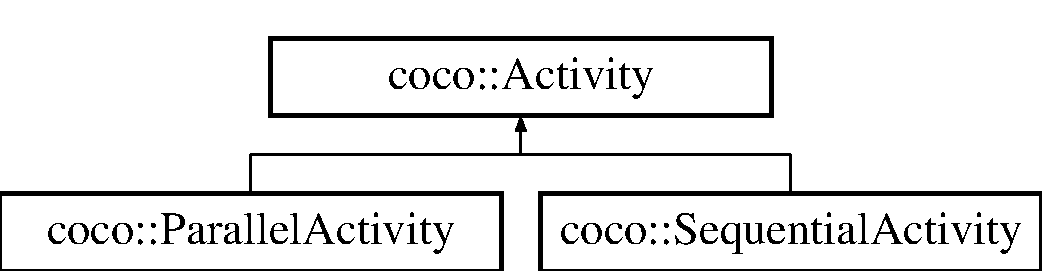
\includegraphics[height=2.000000cm]{classcoco_1_1_activity}
\end{center}
\end{figure}
\subsection*{Public Member Functions}
\begin{DoxyCompactItemize}
\item 
\hypertarget{classcoco_1_1_activity_af87c30a3b206f7f77c832f4e1e2c1d81}{\hyperlink{classcoco_1_1_activity_af87c30a3b206f7f77c832f4e1e2c1d81}{Activity} (\hyperlink{structcoco_1_1_schedule_policy}{Schedule\-Policy} policy, std\-::shared\-\_\-ptr$<$ \hyperlink{classcoco_1_1_runnable_interface}{Runnable\-Interface} $>$ r)}\label{classcoco_1_1_activity_af87c30a3b206f7f77c832f4e1e2c1d81}

\begin{DoxyCompactList}\small\item\em specify the execution policy and the \hyperlink{classcoco_1_1_runnable_interface}{Runnable\-Interface} to be executed \end{DoxyCompactList}\item 
\hypertarget{classcoco_1_1_activity_a542dbe1300aa4f03b165dbe4edeb96dd}{virtual void \hyperlink{classcoco_1_1_activity_a542dbe1300aa4f03b165dbe4edeb96dd}{start} ()=0}\label{classcoco_1_1_activity_a542dbe1300aa4f03b165dbe4edeb96dd}

\begin{DoxyCompactList}\small\item\em Start the activity. \end{DoxyCompactList}\item 
\hypertarget{classcoco_1_1_activity_a5c81aa82b5987e3ef5c56affdaefbbaf}{virtual void \hyperlink{classcoco_1_1_activity_a5c81aa82b5987e3ef5c56affdaefbbaf}{stop} ()=0}\label{classcoco_1_1_activity_a5c81aa82b5987e3ef5c56affdaefbbaf}

\begin{DoxyCompactList}\small\item\em Stop the activity. \end{DoxyCompactList}\item 
\hypertarget{classcoco_1_1_activity_a4359a691fe84c7334a6e956cd56b7752}{virtual bool {\bfseries is\-Periodic} ()}\label{classcoco_1_1_activity_a4359a691fe84c7334a6e956cd56b7752}

\item 
\hypertarget{classcoco_1_1_activity_ad270583e0ec466f87df956bd7673f554}{virtual void \hyperlink{classcoco_1_1_activity_ad270583e0ec466f87df956bd7673f554}{trigger} ()=0}\label{classcoco_1_1_activity_ad270583e0ec466f87df956bd7673f554}

\begin{DoxyCompactList}\small\item\em in case of a T\-R\-I\-G\-G\-E\-R activity starts one step of the execution \end{DoxyCompactList}\item 
\hypertarget{classcoco_1_1_activity_a8a1182e9e8649223df1e0ec4e3648395}{virtual void \hyperlink{classcoco_1_1_activity_a8a1182e9e8649223df1e0ec4e3648395}{entry} ()=0}\label{classcoco_1_1_activity_a8a1182e9e8649223df1e0ec4e3648395}

\begin{DoxyCompactList}\small\item\em main execution function \end{DoxyCompactList}\item 
\hypertarget{classcoco_1_1_activity_a99600e19dc7279629e291c821e98d522}{void \hyperlink{classcoco_1_1_activity_a99600e19dc7279629e291c821e98d522}{init} ()}\label{classcoco_1_1_activity_a99600e19dc7279629e291c821e98d522}

\begin{DoxyCompactList}\small\item\em initialize the acrivity and the Engine \end{DoxyCompactList}\item 
\hypertarget{classcoco_1_1_activity_aca34cad2b6211a66efe5bbdf4db5aa44}{bool {\bfseries is\-Active} ()}\label{classcoco_1_1_activity_aca34cad2b6211a66efe5bbdf4db5aa44}

\item 
\hypertarget{classcoco_1_1_activity_a9c2f3c05e3416e4617496de06c83a00b}{Schedule\-Policy\-::\-Policy {\bfseries get\-Policy\-Type} ()}\label{classcoco_1_1_activity_a9c2f3c05e3416e4617496de06c83a00b}

\end{DoxyCompactItemize}
\subsection*{Protected Attributes}
\begin{DoxyCompactItemize}
\item 
\hypertarget{classcoco_1_1_activity_a5f2a9c45be825f79905581e237b1bcbd}{std\-::shared\-\_\-ptr\\*
$<$ \hyperlink{classcoco_1_1_runnable_interface}{Runnable\-Interface} $>$ {\bfseries runnable\-\_\-}}\label{classcoco_1_1_activity_a5f2a9c45be825f79905581e237b1bcbd}

\item 
\hypertarget{classcoco_1_1_activity_a75a9fe827a532ab36696487b0ca3d166}{\hyperlink{structcoco_1_1_schedule_policy}{Schedule\-Policy} {\bfseries policy\-\_\-}}\label{classcoco_1_1_activity_a75a9fe827a532ab36696487b0ca3d166}

\item 
\hypertarget{classcoco_1_1_activity_aef80c256f45b789d987673a4f350907e}{bool {\bfseries active\-\_\-}}\label{classcoco_1_1_activity_aef80c256f45b789d987673a4f350907e}

\item 
\hypertarget{classcoco_1_1_activity_ac7e15c803c0f74c88ac5ae1f489ee9f3}{std\-::atomic$<$ bool $>$ {\bfseries stopping\-\_\-}}\label{classcoco_1_1_activity_ac7e15c803c0f74c88ac5ae1f489ee9f3}

\end{DoxyCompactItemize}


\subsection{Detailed Description}
Base class for something that loops or is activated

T\-O\-D\-O\-: ownership T\-O\-D\-O\-: specialized for\-: Sequential and Parallel 

The documentation for this class was generated from the following file\-:\begin{DoxyCompactItemize}
\item 
src/ezoro.\-hpp\end{DoxyCompactItemize}

\hypertarget{classcoco_1_1_attribute}{}\section{coco\+:\+:Attribute$<$ T $>$ Class Template Reference}
\label{classcoco_1_1_attribute}\index{coco\+::\+Attribute$<$ T $>$@{coco\+::\+Attribute$<$ T $>$}}


template spec of attribute  




{\ttfamily \#include $<$coco\+\_\+core.\+hpp$>$}

Inheritance diagram for coco\+:\+:Attribute$<$ T $>$\+:\begin{figure}[H]
\begin{center}
\leavevmode
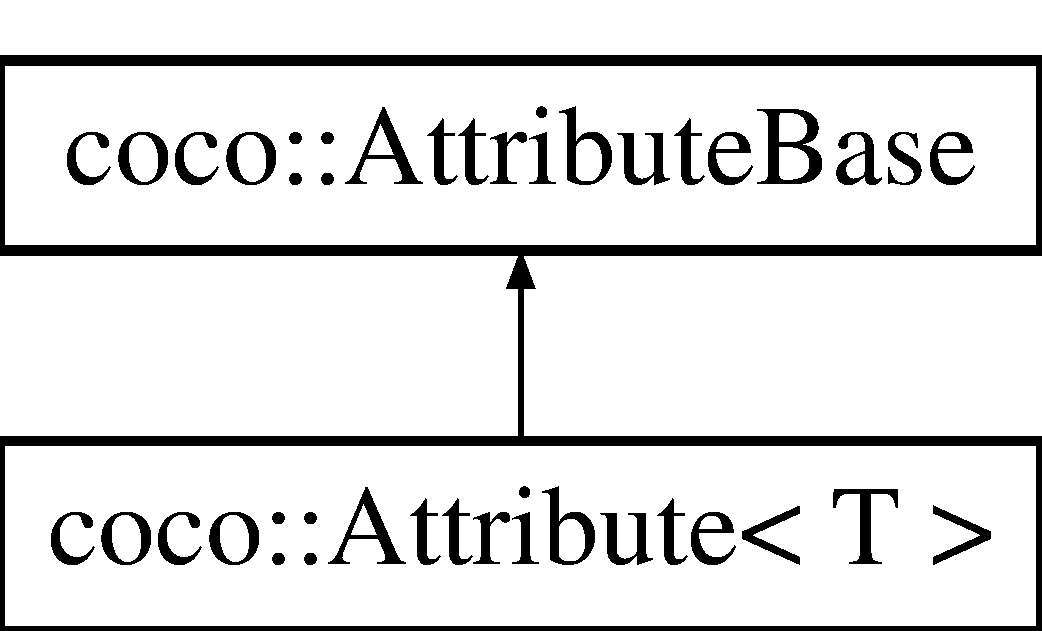
\includegraphics[height=2.000000cm]{classcoco_1_1_attribute}
\end{center}
\end{figure}
\subsection*{Public Member Functions}
\begin{DoxyCompactItemize}
\item 
\hypertarget{classcoco_1_1_attribute_affcacf8fe8cbb263d456b6ebcb11ce3f}{}{\bfseries Attribute} (\hyperlink{classcoco_1_1_task_context}{Task\+Context} $\ast$p, std\+::string name, T \&rvalue)\label{classcoco_1_1_attribute_affcacf8fe8cbb263d456b6ebcb11ce3f}

\item 
\hypertarget{classcoco_1_1_attribute_a3593a7754010b3525e7ee2b457728d44}{}\hyperlink{classcoco_1_1_attribute}{Attribute} \& {\bfseries operator=} (const T \&x)\label{classcoco_1_1_attribute_a3593a7754010b3525e7ee2b457728d44}

\item 
\hypertarget{classcoco_1_1_attribute_a5e93340edc07fbcf413cbc3b61045e27}{}virtual const std\+::type\+\_\+info \& {\bfseries assig} () override\label{classcoco_1_1_attribute_a5e93340edc07fbcf413cbc3b61045e27}

\item 
\hypertarget{classcoco_1_1_attribute_ad170afa18295d7b00c1d2e8b9561a7b8}{}virtual void {\bfseries set\+Value} (const std\+::string \&c\+\_\+value) override\label{classcoco_1_1_attribute_ad170afa18295d7b00c1d2e8b9561a7b8}

\item 
\hypertarget{classcoco_1_1_attribute_aad989eaf82993b857ccde4f2226f1c07}{}virtual void $\ast$ {\bfseries value} () override\label{classcoco_1_1_attribute_aad989eaf82993b857ccde4f2226f1c07}

\item 
\hypertarget{classcoco_1_1_attribute_a1c51ca833bf8b35d3faed63fb9209958}{}virtual std\+::string {\bfseries to\+String} () override\label{classcoco_1_1_attribute_a1c51ca833bf8b35d3faed63fb9209958}

\end{DoxyCompactItemize}
\subsection*{Private Attributes}
\begin{DoxyCompactItemize}
\item 
\hypertarget{classcoco_1_1_attribute_abb200730d0b02d75077c5e4875af6482}{}T \& {\bfseries value\+\_\+}\label{classcoco_1_1_attribute_abb200730d0b02d75077c5e4875af6482}

\end{DoxyCompactItemize}


\subsection{Detailed Description}
\subsubsection*{template$<$class T$>$class coco\+::\+Attribute$<$ T $>$}

template spec of attribute 

The documentation for this class was generated from the following file\+:\begin{DoxyCompactItemize}
\item 
src/coco\+\_\+core.\+hpp\end{DoxyCompactItemize}

\hypertarget{classcoco_1_1_attribute_base}{}\section{coco\+:\+:Attribute\+Base Class Reference}
\label{classcoco_1_1_attribute_base}\index{coco\+::\+Attribute\+Base@{coco\+::\+Attribute\+Base}}


run-\/time value  




{\ttfamily \#include $<$coco\+\_\+core.\+hpp$>$}

Inheritance diagram for coco\+:\+:Attribute\+Base\+:\begin{figure}[H]
\begin{center}
\leavevmode
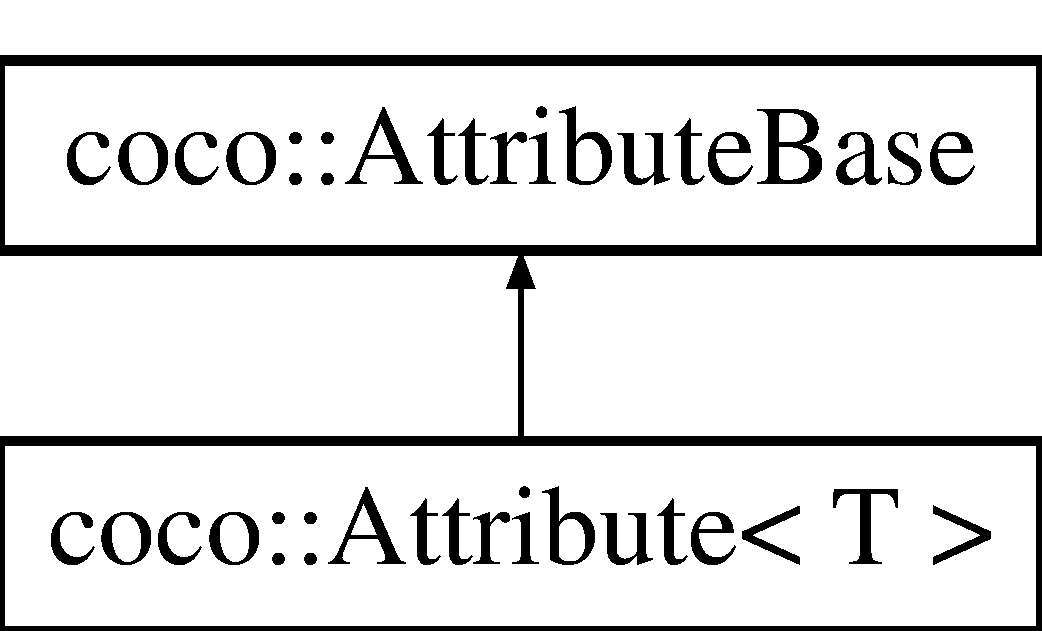
\includegraphics[height=2.000000cm]{classcoco_1_1_attribute_base}
\end{center}
\end{figure}
\subsection*{Public Member Functions}
\begin{DoxyCompactItemize}
\item 
\hypertarget{classcoco_1_1_attribute_base_a91ba95249f0d57b4eb18fbc65649d74f}{}{\bfseries Attribute\+Base} (\hyperlink{classcoco_1_1_task_context}{Task\+Context} $\ast$p, const std\+::string \&name)\label{classcoco_1_1_attribute_base_a91ba95249f0d57b4eb18fbc65649d74f}

\item 
\hypertarget{classcoco_1_1_attribute_base_a18fdc12e5d8c59672d94d4dbc85a1508}{}virtual void {\bfseries set\+Value} (const std\+::string \&c\+\_\+value)=0\label{classcoco_1_1_attribute_base_a18fdc12e5d8c59672d94d4dbc85a1508}

\item 
\hypertarget{classcoco_1_1_attribute_base_aa13d350700c8e427588996cc1d6e13f7}{}virtual const std\+::type\+\_\+info \& {\bfseries assig} ()=0\label{classcoco_1_1_attribute_base_aa13d350700c8e427588996cc1d6e13f7}

\item 
\hypertarget{classcoco_1_1_attribute_base_a3a036a12d37b626b32029720d3319989}{}virtual void $\ast$ {\bfseries value} ()=0\label{classcoco_1_1_attribute_base_a3a036a12d37b626b32029720d3319989}

\item 
\hypertarget{classcoco_1_1_attribute_base_aebdb7487eae12da4423f2c89f6b96ba6}{}virtual std\+::string {\bfseries to\+String} ()=0\label{classcoco_1_1_attribute_base_aebdb7487eae12da4423f2c89f6b96ba6}

\item 
\hypertarget{classcoco_1_1_attribute_base_a145d59a25865b63c1911677fb672ecfc}{}const std\+::string \& {\bfseries name} () const \label{classcoco_1_1_attribute_base_a145d59a25865b63c1911677fb672ecfc}

\item 
\hypertarget{classcoco_1_1_attribute_base_a218ce4d45c5c3a061e141f9b33f4412d}{}void {\bfseries name} (const std\+::string \&n)\label{classcoco_1_1_attribute_base_a218ce4d45c5c3a061e141f9b33f4412d}

\item 
\hypertarget{classcoco_1_1_attribute_base_ac593f2318da763db052ee1436f862cde}{}const std\+::string \& \hyperlink{classcoco_1_1_attribute_base_ac593f2318da763db052ee1436f862cde}{doc} () const \label{classcoco_1_1_attribute_base_ac593f2318da763db052ee1436f862cde}

\begin{DoxyCompactList}\small\item\em associated documentation \end{DoxyCompactList}\item 
\hypertarget{classcoco_1_1_attribute_base_aa58d9320fa9d8a368b1bb242b47a0d3e}{}void \hyperlink{classcoco_1_1_attribute_base_aa58d9320fa9d8a368b1bb242b47a0d3e}{doc} (const std\+::string \&d)\label{classcoco_1_1_attribute_base_aa58d9320fa9d8a368b1bb242b47a0d3e}

\begin{DoxyCompactList}\small\item\em stores doc \end{DoxyCompactList}\item 
\hypertarget{classcoco_1_1_attribute_base_a7a8d1f2d64f8087b5a582ca88aaaa7a9}{}{\footnotesize template$<$class T $>$ }\\T \& {\bfseries as} ()\label{classcoco_1_1_attribute_base_a7a8d1f2d64f8087b5a582ca88aaaa7a9}

\end{DoxyCompactItemize}
\subsection*{Private Attributes}
\begin{DoxyCompactItemize}
\item 
\hypertarget{classcoco_1_1_attribute_base_afcfc37b436c721506d1c70fa62cfdfc7}{}std\+::string {\bfseries name\+\_\+}\label{classcoco_1_1_attribute_base_afcfc37b436c721506d1c70fa62cfdfc7}

\item 
\hypertarget{classcoco_1_1_attribute_base_ab4f73c19a580d3c063757fb8573205eb}{}std\+::string {\bfseries doc\+\_\+}\label{classcoco_1_1_attribute_base_ab4f73c19a580d3c063757fb8573205eb}

\end{DoxyCompactItemize}


\subsection{Detailed Description}
run-\/time value 

The documentation for this class was generated from the following files\+:\begin{DoxyCompactItemize}
\item 
src/coco\+\_\+core.\+hpp\item 
src/coco\+\_\+core.\+cpp\end{DoxyCompactItemize}

\input{classcoco_1_1_coco_launcher}
\input{classcoco_1_1_coco_loader}
\hypertarget{classcoco_1_1_component_registry}{\section{coco\-:\-:Component\-Registry Class Reference}
\label{classcoco_1_1_component_registry}\index{coco\-::\-Component\-Registry@{coco\-::\-Component\-Registry}}
}


{\ttfamily \#include $<$ezoro.\-hpp$>$}

\subsection*{Static Public Member Functions}
\begin{DoxyCompactItemize}
\item 
\hypertarget{classcoco_1_1_component_registry_adf767122683bad2ca7f863be912589d3}{static \hyperlink{classcoco_1_1_task_context}{Task\-Context} $\ast$ \hyperlink{classcoco_1_1_component_registry_adf767122683bad2ca7f863be912589d3}{create} (const char $\ast$name)}\label{classcoco_1_1_component_registry_adf767122683bad2ca7f863be912589d3}

\begin{DoxyCompactList}\small\item\em creates a component by name \end{DoxyCompactList}\item 
\hypertarget{classcoco_1_1_component_registry_ac242dec3121dc83d32638c092541889f}{static void \hyperlink{classcoco_1_1_component_registry_ac242dec3121dc83d32638c092541889f}{add\-Spec} (\hyperlink{classcoco_1_1_component_spec}{Component\-Spec} $\ast$s)}\label{classcoco_1_1_component_registry_ac242dec3121dc83d32638c092541889f}

\begin{DoxyCompactList}\small\item\em adds a specification \end{DoxyCompactList}\item 
\hypertarget{classcoco_1_1_component_registry_ad665d9355353a110af2822f2f3ff7563}{static bool \hyperlink{classcoco_1_1_component_registry_ad665d9355353a110af2822f2f3ff7563}{add\-Library} (const char $\ast$)}\label{classcoco_1_1_component_registry_ad665d9355353a110af2822f2f3ff7563}

\begin{DoxyCompactList}\small\item\em adds a library \end{DoxyCompactList}\item 
\hypertarget{classcoco_1_1_component_registry_a2bdf8f5d4e827326baec571ee6e7e17c}{static void \hyperlink{classcoco_1_1_component_registry_a2bdf8f5d4e827326baec571ee6e7e17c}{alias} (const char $\ast$newname, const char $\ast$oldname)}\label{classcoco_1_1_component_registry_a2bdf8f5d4e827326baec571ee6e7e17c}

\begin{DoxyCompactList}\small\item\em defines an alias. note that oldname should be present \end{DoxyCompactList}\end{DoxyCompactItemize}
\subsection*{Private Member Functions}
\begin{DoxyCompactItemize}
\item 
\hypertarget{classcoco_1_1_component_registry_a948e4e55ecc8816bb00adef0e18732b3}{\hyperlink{classcoco_1_1_task_context}{Task\-Context} $\ast$ {\bfseries create\-\_\-} (const char $\ast$name)}\label{classcoco_1_1_component_registry_a948e4e55ecc8816bb00adef0e18732b3}

\item 
\hypertarget{classcoco_1_1_component_registry_a3a0a94247eecb4a2ebdac0ec559745ff}{void {\bfseries add\-Spec\-\_\-} (\hyperlink{classcoco_1_1_component_spec}{Component\-Spec} $\ast$s)}\label{classcoco_1_1_component_registry_a3a0a94247eecb4a2ebdac0ec559745ff}

\item 
\hypertarget{classcoco_1_1_component_registry_adc252eec7576f3bda778cecb3662d2f5}{bool {\bfseries add\-Library\-\_\-} (const char $\ast$)}\label{classcoco_1_1_component_registry_adc252eec7576f3bda778cecb3662d2f5}

\item 
\hypertarget{classcoco_1_1_component_registry_a31855c1fe9a7697b8225e5108c92891e}{void {\bfseries alias\-\_\-} (const char $\ast$newname, const char $\ast$oldname)}\label{classcoco_1_1_component_registry_a31855c1fe9a7697b8225e5108c92891e}

\end{DoxyCompactItemize}
\subsection*{Static Private Member Functions}
\begin{DoxyCompactItemize}
\item 
\hypertarget{classcoco_1_1_component_registry_a1ada72627a6e3daf61115a20fdfc00f5}{static \hyperlink{classcoco_1_1_component_registry}{Component\-Registry} \& {\bfseries get} ()}\label{classcoco_1_1_component_registry_a1ada72627a6e3daf61115a20fdfc00f5}

\end{DoxyCompactItemize}
\subsection*{Private Attributes}
\begin{DoxyCompactItemize}
\item 
\hypertarget{classcoco_1_1_component_registry_a28ce74205cca34a3d03c7916629c2f58}{std\-::map$<$ std\-::string, \\*
\hyperlink{classcoco_1_1_component_spec}{Component\-Spec} $\ast$ $>$ {\bfseries specs}}\label{classcoco_1_1_component_registry_a28ce74205cca34a3d03c7916629c2f58}

\item 
\hypertarget{classcoco_1_1_component_registry_a62eba9c111c9df9405d5c0c7500c91b1}{std\-::set$<$ std\-::string $>$ {\bfseries libs}}\label{classcoco_1_1_component_registry_a62eba9c111c9df9405d5c0c7500c91b1}

\item 
\hypertarget{classcoco_1_1_component_registry_aab792483941bb3b14655cf297fe44034}{std\-::map$<$ std\-::string, \\*
std\-::shared\-\_\-ptr$<$ \hyperlink{classcoco_1_1_task_context}{Task\-Context} $>$ $>$ {\bfseries contexts}}\label{classcoco_1_1_component_registry_aab792483941bb3b14655cf297fe44034}

\end{DoxyCompactItemize}


\subsection{Detailed Description}
Component Registry that is singleton per each exec or library. Then when the component library is loaded the singleton is replacedù

add the addition of a full path to automatically add libraries 

The documentation for this class was generated from the following files\-:\begin{DoxyCompactItemize}
\item 
src/ezoro.\-hpp\item 
src/ezoro.\-cpp\end{DoxyCompactItemize}

\hypertarget{classcoco_1_1_component_spec}{}\section{coco\+:\+:Component\+Spec Class Reference}
\label{classcoco_1_1_component_spec}\index{coco\+::\+Component\+Spec@{coco\+::\+Component\+Spec}}


Specification of the component, as created by the macro.  




{\ttfamily \#include $<$coco\+\_\+core.\+hpp$>$}

\subsection*{Public Types}
\begin{DoxyCompactItemize}
\item 
\hypertarget{classcoco_1_1_component_spec_a3f8ee2e4603484b700fef040758a64e9}{}typedef std\+::function$<$ \hyperlink{classcoco_1_1_task_context}{Task\+Context} $\ast$()$>$ {\bfseries makefx\+\_\+t}\label{classcoco_1_1_component_spec_a3f8ee2e4603484b700fef040758a64e9}

\end{DoxyCompactItemize}
\subsection*{Public Member Functions}
\begin{DoxyCompactItemize}
\item 
\hypertarget{classcoco_1_1_component_spec_a1588367e549ef93c9484084954a44cc7}{}{\bfseries Component\+Spec} (const std\+::string \&name, makefx\+\_\+t fx)\label{classcoco_1_1_component_spec_a1588367e549ef93c9484084954a44cc7}

\end{DoxyCompactItemize}
\subsection*{Public Attributes}
\begin{DoxyCompactItemize}
\item 
\hypertarget{classcoco_1_1_component_spec_a47822521036decc06ea24b6d238980d0}{}std\+::string {\bfseries name\+\_\+}\label{classcoco_1_1_component_spec_a47822521036decc06ea24b6d238980d0}

\item 
\hypertarget{classcoco_1_1_component_spec_ab8f5984058f581717ab0cefc8316094c}{}makefx\+\_\+t {\bfseries fx\+\_\+}\label{classcoco_1_1_component_spec_ab8f5984058f581717ab0cefc8316094c}

\end{DoxyCompactItemize}


\subsection{Detailed Description}
Specification of the component, as created by the macro. 

The documentation for this class was generated from the following files\+:\begin{DoxyCompactItemize}
\item 
src/coco\+\_\+core.\+hpp\item 
src/coco\+\_\+core.\+cpp\end{DoxyCompactItemize}

\hypertarget{classcoco_1_1_connection_base}{}\section{coco\+:\+:Connection\+Base Class Reference}
\label{classcoco_1_1_connection_base}\index{coco\+::\+Connection\+Base@{coco\+::\+Connection\+Base}}


{\ttfamily \#include $<$coco\+\_\+core.\+hpp$>$}

Inheritance diagram for coco\+:\+:Connection\+Base\+:\begin{figure}[H]
\begin{center}
\leavevmode
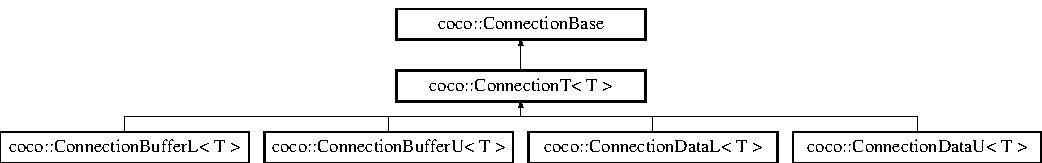
\includegraphics[height=2.187500cm]{classcoco_1_1_connection_base}
\end{center}
\end{figure}
\subsection*{Public Member Functions}
\begin{DoxyCompactItemize}
\item 
\hypertarget{classcoco_1_1_connection_base_aecb0c585cd9313e30f7d592ed08c6059}{}\hyperlink{classcoco_1_1_connection_base_aecb0c585cd9313e30f7d592ed08c6059}{Connection\+Base} (\hyperlink{classcoco_1_1_port_base}{Port\+Base} $\ast$in, \hyperlink{classcoco_1_1_port_base}{Port\+Base} $\ast$out, \hyperlink{structcoco_1_1_connection_policy}{Connection\+Policy} policy)\label{classcoco_1_1_connection_base_aecb0c585cd9313e30f7d592ed08c6059}

\begin{DoxyCompactList}\small\item\em Constructor. \end{DoxyCompactList}\item 
bool \hyperlink{classcoco_1_1_connection_base_aca4a3ab712e816089a1ee35cb0546d8d}{has\+New\+Data} () const 
\item 
\hypertarget{classcoco_1_1_connection_base_ac30b073f630b45c3e7f272378dd8945c}{}bool {\bfseries has\+Component} (const std\+::string \&name) const \label{classcoco_1_1_connection_base_ac30b073f630b45c3e7f272378dd8945c}

\end{DoxyCompactItemize}
\subsection*{Protected Member Functions}
\begin{DoxyCompactItemize}
\item 
\hypertarget{classcoco_1_1_connection_base_a48861f5913490df52b2a741a51275293}{}void \hyperlink{classcoco_1_1_connection_base_a48861f5913490df52b2a741a51275293}{trigger} ()\label{classcoco_1_1_connection_base_a48861f5913490df52b2a741a51275293}

\begin{DoxyCompactList}\small\item\em Trigger the port to communicate new data is present. \end{DoxyCompactList}\end{DoxyCompactItemize}
\subsection*{Protected Attributes}
\begin{DoxyCompactItemize}
\item 
\hypertarget{classcoco_1_1_connection_base_a526b0954719f06db131e3e5d00687aef}{}\hyperlink{namespacecoco_a057be58377e415c9be98c1dc5c8426ad}{Flow\+Status} {\bfseries data\+\_\+status\+\_\+}\label{classcoco_1_1_connection_base_a526b0954719f06db131e3e5d00687aef}

\item 
\hypertarget{classcoco_1_1_connection_base_a64e625d75ed25b17039caa39847a45d9}{}\hyperlink{structcoco_1_1_connection_policy}{Connection\+Policy} \hyperlink{classcoco_1_1_connection_base_a64e625d75ed25b17039caa39847a45d9}{policy\+\_\+}\label{classcoco_1_1_connection_base_a64e625d75ed25b17039caa39847a45d9}

\begin{DoxyCompactList}\small\item\em status of the data in the container \end{DoxyCompactList}\item 
\hypertarget{classcoco_1_1_connection_base_aa8866747c7325f4605d42d53bd0224ef}{}\hyperlink{classcoco_1_1_port_base}{Port\+Base} $\ast$ \hyperlink{classcoco_1_1_connection_base_aa8866747c7325f4605d42d53bd0224ef}{input\+\_\+} = 0\label{classcoco_1_1_connection_base_aa8866747c7325f4605d42d53bd0224ef}

\begin{DoxyCompactList}\small\item\em policy for data management \end{DoxyCompactList}\item 
\hypertarget{classcoco_1_1_connection_base_a2f5548815a384f99068543b94a9750f5}{}\hyperlink{classcoco_1_1_port_base}{Port\+Base} $\ast$ \hyperlink{classcoco_1_1_connection_base_a2f5548815a384f99068543b94a9750f5}{output\+\_\+} = 0\label{classcoco_1_1_connection_base_a2f5548815a384f99068543b94a9750f5}

\begin{DoxyCompactList}\small\item\em input port untyped \end{DoxyCompactList}\end{DoxyCompactItemize}


\subsection{Detailed Description}
Base class for connections 

\subsection{Member Function Documentation}
\hypertarget{classcoco_1_1_connection_base_aca4a3ab712e816089a1ee35cb0546d8d}{}\index{coco\+::\+Connection\+Base@{coco\+::\+Connection\+Base}!has\+New\+Data@{has\+New\+Data}}
\index{has\+New\+Data@{has\+New\+Data}!coco\+::\+Connection\+Base@{coco\+::\+Connection\+Base}}
\subsubsection[{has\+New\+Data}]{\setlength{\rightskip}{0pt plus 5cm}bool coco\+::\+Connection\+Base\+::has\+New\+Data (
\begin{DoxyParamCaption}
{}
\end{DoxyParamCaption}
) const\hspace{0.3cm}{\ttfamily [inline]}}\label{classcoco_1_1_connection_base_aca4a3ab712e816089a1ee35cb0546d8d}
\begin{DoxyReturn}{Returns}
N\+E\+W\+\_\+\+D\+A\+T\+A if new data is present in the Input port 
\end{DoxyReturn}


The documentation for this class was generated from the following files\+:\begin{DoxyCompactItemize}
\item 
src/coco\+\_\+core.\+hpp\item 
src/coco\+\_\+core.\+cpp\end{DoxyCompactItemize}

\hypertarget{classcoco_1_1_connection_buffer_l}{\section{coco\-:\-:Connection\-Buffer\-L$<$ T $>$ Class Template Reference}
\label{classcoco_1_1_connection_buffer_l}\index{coco\-::\-Connection\-Buffer\-L$<$ T $>$@{coco\-::\-Connection\-Buffer\-L$<$ T $>$}}
}


Specialized class for the type T to manage Connection\-Policy\-::\-B\-U\-F\-F\-E\-R/\-C\-I\-R\-C\-U\-L\-A\-R\-\_\-\-B\-U\-F\-F\-E\-R Connection\-Policy\-::\-L\-O\-C\-K\-E\-D.  




{\ttfamily \#include $<$ezoro.\-hpp$>$}

Inheritance diagram for coco\-:\-:Connection\-Buffer\-L$<$ T $>$\-:\begin{figure}[H]
\begin{center}
\leavevmode
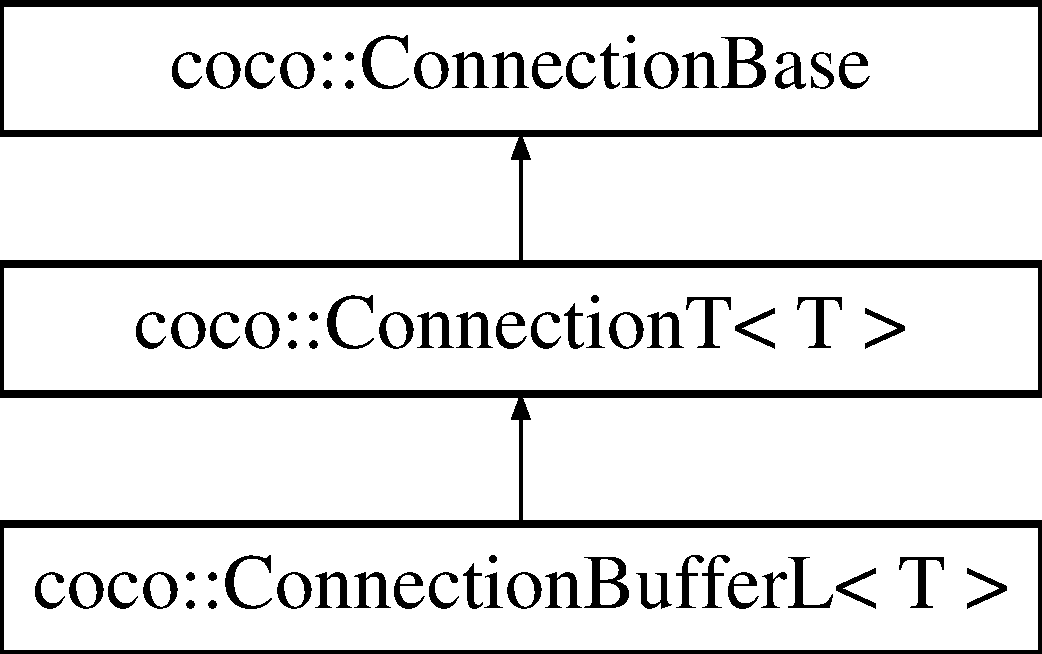
\includegraphics[height=3.000000cm]{classcoco_1_1_connection_buffer_l}
\end{center}
\end{figure}
\subsection*{Public Member Functions}
\begin{DoxyCompactItemize}
\item 
\hypertarget{classcoco_1_1_connection_buffer_l_af15b0bc37247b71bef3b272b2c3aae8d}{\hyperlink{classcoco_1_1_connection_buffer_l_af15b0bc37247b71bef3b272b2c3aae8d}{Connection\-Buffer\-L} (\hyperlink{classcoco_1_1_input_port}{Input\-Port}$<$ T $>$ $\ast$in, \hyperlink{classcoco_1_1_output_port}{Output\-Port}$<$ T $>$ $\ast$out, \hyperlink{structcoco_1_1_connection_policy}{Connection\-Policy} policy)}\label{classcoco_1_1_connection_buffer_l_af15b0bc37247b71bef3b272b2c3aae8d}

\begin{DoxyCompactList}\small\item\em Simply call Connection\-T$<$\-T$>$ constructor. \end{DoxyCompactList}\item 
\hypertarget{classcoco_1_1_connection_buffer_l_a8619c883cd8777a51ed52ddee3693968}{virtual \hyperlink{namespacecoco_a057be58377e415c9be98c1dc5c8426ad}{Flow\-Status} {\bfseries get\-Newest\-Data} (T \&data)}\label{classcoco_1_1_connection_buffer_l_a8619c883cd8777a51ed52ddee3693968}

\item 
\hypertarget{classcoco_1_1_connection_buffer_l_a54f7cf59bbf27a4ce0beee0c231c0bf9}{virtual \hyperlink{namespacecoco_a057be58377e415c9be98c1dc5c8426ad}{Flow\-Status} \hyperlink{classcoco_1_1_connection_buffer_l_a54f7cf59bbf27a4ce0beee0c231c0bf9}{get\-Data} (T \&data) override}\label{classcoco_1_1_connection_buffer_l_a54f7cf59bbf27a4ce0beee0c231c0bf9}

\begin{DoxyCompactList}\small\item\em If there is new data in the container retrive it. \end{DoxyCompactList}\item 
\hypertarget{classcoco_1_1_connection_buffer_l_a0f719a13d365fb116bce2477940bdb2e}{virtual bool \hyperlink{classcoco_1_1_connection_buffer_l_a0f719a13d365fb116bce2477940bdb2e}{add\-Data} (T \&input) override}\label{classcoco_1_1_connection_buffer_l_a0f719a13d365fb116bce2477940bdb2e}

\begin{DoxyCompactList}\small\item\em Add data to the container. If the input port is of type event trigger it to wake up the execution. \end{DoxyCompactList}\end{DoxyCompactItemize}
\subsection*{Private Attributes}
\begin{DoxyCompactItemize}
\item 
\hypertarget{classcoco_1_1_connection_buffer_l_ab5751072ac523ef93ee8d91b931665fc}{boost\-::circular\-\_\-buffer$<$ T $>$ {\bfseries buffer\-\_\-}}\label{classcoco_1_1_connection_buffer_l_ab5751072ac523ef93ee8d91b931665fc}

\item 
\hypertarget{classcoco_1_1_connection_buffer_l_a11e0301f390b46e9c0cc92d7d8634f7a}{std\-::mutex {\bfseries mutex\-\_\-t\-\_\-}}\label{classcoco_1_1_connection_buffer_l_a11e0301f390b46e9c0cc92d7d8634f7a}

\end{DoxyCompactItemize}
\subsection*{Additional Inherited Members}


\subsection{Detailed Description}
\subsubsection*{template$<$class T$>$class coco\-::\-Connection\-Buffer\-L$<$ T $>$}

Specialized class for the type T to manage Connection\-Policy\-::\-B\-U\-F\-F\-E\-R/\-C\-I\-R\-C\-U\-L\-A\-R\-\_\-\-B\-U\-F\-F\-E\-R Connection\-Policy\-::\-L\-O\-C\-K\-E\-D. 

The documentation for this class was generated from the following file\-:\begin{DoxyCompactItemize}
\item 
src/ezoro.\-hpp\end{DoxyCompactItemize}

\hypertarget{classcoco_1_1_connection_buffer_u}{\section{coco\-:\-:Connection\-Buffer\-U$<$ T $>$ Class Template Reference}
\label{classcoco_1_1_connection_buffer_u}\index{coco\-::\-Connection\-Buffer\-U$<$ T $>$@{coco\-::\-Connection\-Buffer\-U$<$ T $>$}}
}


Specialized class for the type T to manage Connection\-Policy\-::\-B\-U\-F\-F\-E\-R/\-C\-I\-R\-C\-U\-L\-A\-R\-\_\-\-B\-U\-F\-F\-E\-R Connection\-Policy\-::\-U\-N\-S\-Y\-N\-C.  




{\ttfamily \#include $<$ezoro.\-hpp$>$}

Inheritance diagram for coco\-:\-:Connection\-Buffer\-U$<$ T $>$\-:\begin{figure}[H]
\begin{center}
\leavevmode
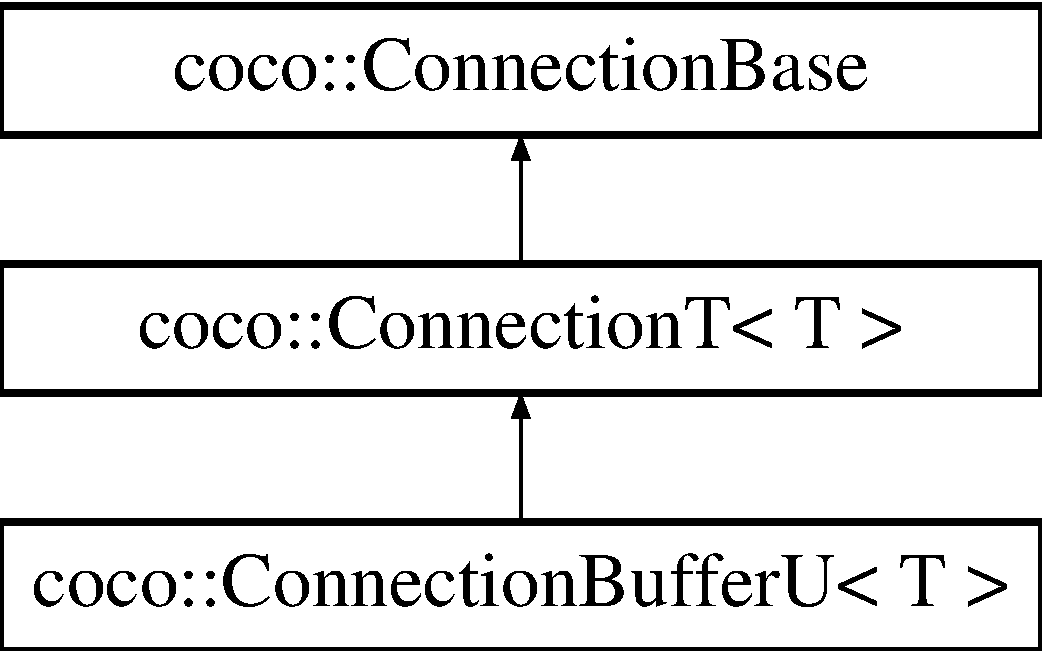
\includegraphics[height=3.000000cm]{classcoco_1_1_connection_buffer_u}
\end{center}
\end{figure}
\subsection*{Public Member Functions}
\begin{DoxyCompactItemize}
\item 
\hypertarget{classcoco_1_1_connection_buffer_u_aebbc3c18dd8b27f11dcdc83b15f24770}{\hyperlink{classcoco_1_1_connection_buffer_u_aebbc3c18dd8b27f11dcdc83b15f24770}{Connection\-Buffer\-U} (\hyperlink{classcoco_1_1_input_port}{Input\-Port}$<$ T $>$ $\ast$in, \hyperlink{classcoco_1_1_output_port}{Output\-Port}$<$ T $>$ $\ast$out, \hyperlink{structcoco_1_1_connection_policy}{Connection\-Policy} policy)}\label{classcoco_1_1_connection_buffer_u_aebbc3c18dd8b27f11dcdc83b15f24770}

\begin{DoxyCompactList}\small\item\em Simply call Connection\-T$<$\-T$>$ constructor. \end{DoxyCompactList}\item 
\hypertarget{classcoco_1_1_connection_buffer_u_a853c1a94c0d2e3c937298860a5c8cbe3}{virtual \hyperlink{namespacecoco_a057be58377e415c9be98c1dc5c8426ad}{Flow\-Status} {\bfseries get\-Newest\-Data} (T \&data)}\label{classcoco_1_1_connection_buffer_u_a853c1a94c0d2e3c937298860a5c8cbe3}

\item 
\hypertarget{classcoco_1_1_connection_buffer_u_ab66b2f4a90e2757c796497f38c8e1695}{virtual \hyperlink{namespacecoco_a057be58377e415c9be98c1dc5c8426ad}{Flow\-Status} \hyperlink{classcoco_1_1_connection_buffer_u_ab66b2f4a90e2757c796497f38c8e1695}{get\-Data} (T \&data) override}\label{classcoco_1_1_connection_buffer_u_ab66b2f4a90e2757c796497f38c8e1695}

\begin{DoxyCompactList}\small\item\em If there is new data in the container retrive it. \end{DoxyCompactList}\item 
\hypertarget{classcoco_1_1_connection_buffer_u_a9cedcd1db28cb0bc70adda82e25538e1}{virtual bool \hyperlink{classcoco_1_1_connection_buffer_u_a9cedcd1db28cb0bc70adda82e25538e1}{add\-Data} (T \&input) override}\label{classcoco_1_1_connection_buffer_u_a9cedcd1db28cb0bc70adda82e25538e1}

\begin{DoxyCompactList}\small\item\em Add data to the container. If the input port is of type event trigger it to wake up the execution. \end{DoxyCompactList}\end{DoxyCompactItemize}
\subsection*{Private Attributes}
\begin{DoxyCompactItemize}
\item 
\hypertarget{classcoco_1_1_connection_buffer_u_af9c42ab03e1318e1adebc63fd598415b}{boost\-::circular\-\_\-buffer$<$ T $>$ {\bfseries buffer\-\_\-}}\label{classcoco_1_1_connection_buffer_u_af9c42ab03e1318e1adebc63fd598415b}

\end{DoxyCompactItemize}
\subsection*{Additional Inherited Members}


\subsection{Detailed Description}
\subsubsection*{template$<$class T$>$class coco\-::\-Connection\-Buffer\-U$<$ T $>$}

Specialized class for the type T to manage Connection\-Policy\-::\-B\-U\-F\-F\-E\-R/\-C\-I\-R\-C\-U\-L\-A\-R\-\_\-\-B\-U\-F\-F\-E\-R Connection\-Policy\-::\-U\-N\-S\-Y\-N\-C. 

The documentation for this class was generated from the following file\-:\begin{DoxyCompactItemize}
\item 
src/ezoro.\-hpp\end{DoxyCompactItemize}

\hypertarget{classcoco_1_1_connection_data_l}{\section{coco\-:\-:Connection\-Data\-L$<$ T $>$ Class Template Reference}
\label{classcoco_1_1_connection_data_l}\index{coco\-::\-Connection\-Data\-L$<$ T $>$@{coco\-::\-Connection\-Data\-L$<$ T $>$}}
}


Specialized class for the type T to manage Connection\-Policy\-::\-D\-A\-T\-A Connection\-Policy\-::\-L\-O\-C\-K\-E\-D.  




{\ttfamily \#include $<$ezoro.\-hpp$>$}

Inheritance diagram for coco\-:\-:Connection\-Data\-L$<$ T $>$\-:\begin{figure}[H]
\begin{center}
\leavevmode
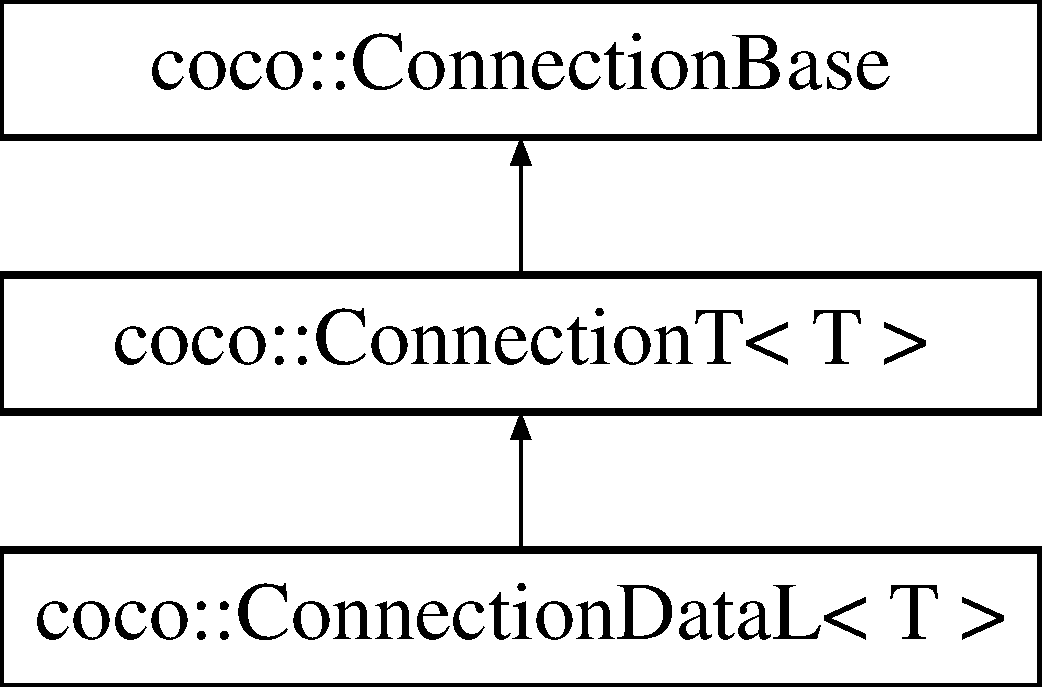
\includegraphics[height=3.000000cm]{classcoco_1_1_connection_data_l}
\end{center}
\end{figure}
\subsection*{Public Member Functions}
\begin{DoxyCompactItemize}
\item 
\hypertarget{classcoco_1_1_connection_data_l_a2e4d4feb75319345f32f2355456105b0}{\hyperlink{classcoco_1_1_connection_data_l_a2e4d4feb75319345f32f2355456105b0}{Connection\-Data\-L} (\hyperlink{classcoco_1_1_input_port}{Input\-Port}$<$ T $>$ $\ast$in, \hyperlink{classcoco_1_1_output_port}{Output\-Port}$<$ T $>$ $\ast$out, \hyperlink{structcoco_1_1_connection_policy}{Connection\-Policy} policy)}\label{classcoco_1_1_connection_data_l_a2e4d4feb75319345f32f2355456105b0}

\begin{DoxyCompactList}\small\item\em Simply call Connection\-T$<$\-T$>$ constructor. \end{DoxyCompactList}\item 
\hypertarget{classcoco_1_1_connection_data_l_a182d9bc170db89f0ed0b4b74abf8e107}{virtual \hyperlink{namespacecoco_a057be58377e415c9be98c1dc5c8426ad}{Flow\-Status} \hyperlink{classcoco_1_1_connection_data_l_a182d9bc170db89f0ed0b4b74abf8e107}{get\-Data} (T \&data) override}\label{classcoco_1_1_connection_data_l_a182d9bc170db89f0ed0b4b74abf8e107}

\begin{DoxyCompactList}\small\item\em If there is new data in the container retrive it. \end{DoxyCompactList}\item 
\hypertarget{classcoco_1_1_connection_data_l_a9c934c06e92dcc6e4442b6ab68b845b7}{virtual bool \hyperlink{classcoco_1_1_connection_data_l_a9c934c06e92dcc6e4442b6ab68b845b7}{add\-Data} (T \&input) override}\label{classcoco_1_1_connection_data_l_a9c934c06e92dcc6e4442b6ab68b845b7}

\begin{DoxyCompactList}\small\item\em Add data to the container. If the input port is of type event trigger it to wake up the execution. \end{DoxyCompactList}\end{DoxyCompactItemize}
\subsection*{Private Attributes}
\begin{DoxyCompactItemize}
\item 
\hypertarget{classcoco_1_1_connection_data_l_a31184a1cae19c735ac431d9f8f56c17f}{\begin{tabbing}
xx\=xx\=xx\=xx\=xx\=xx\=xx\=xx\=xx\=\kill
union \{\\
\>T {\bfseries value\_t\_}\\
\}; }\label{classcoco_1_1_connection_data_l_a31184a1cae19c735ac431d9f8f56c17f}
\\

\end{tabbing}\item 
\hypertarget{classcoco_1_1_connection_data_l_aa290ba1ee648b7bd315b416940aa1765}{std\-::mutex {\bfseries mutex\-\_\-t\-\_\-}}\label{classcoco_1_1_connection_data_l_aa290ba1ee648b7bd315b416940aa1765}

\end{DoxyCompactItemize}
\subsection*{Additional Inherited Members}


\subsection{Detailed Description}
\subsubsection*{template$<$class T$>$class coco\-::\-Connection\-Data\-L$<$ T $>$}

Specialized class for the type T to manage Connection\-Policy\-::\-D\-A\-T\-A Connection\-Policy\-::\-L\-O\-C\-K\-E\-D. 

The documentation for this class was generated from the following file\-:\begin{DoxyCompactItemize}
\item 
src/ezoro.\-hpp\end{DoxyCompactItemize}

\hypertarget{classcoco_1_1_connection_data_u}{\section{coco\-:\-:Connection\-Data\-U$<$ T $>$ Class Template Reference}
\label{classcoco_1_1_connection_data_u}\index{coco\-::\-Connection\-Data\-U$<$ T $>$@{coco\-::\-Connection\-Data\-U$<$ T $>$}}
}


Specialized class for the type T to manage Connection\-Policy\-::\-D\-A\-T\-A Connection\-Policy\-::\-U\-N\-S\-Y\-N\-C.  




{\ttfamily \#include $<$ezoro.\-hpp$>$}

Inheritance diagram for coco\-:\-:Connection\-Data\-U$<$ T $>$\-:\begin{figure}[H]
\begin{center}
\leavevmode
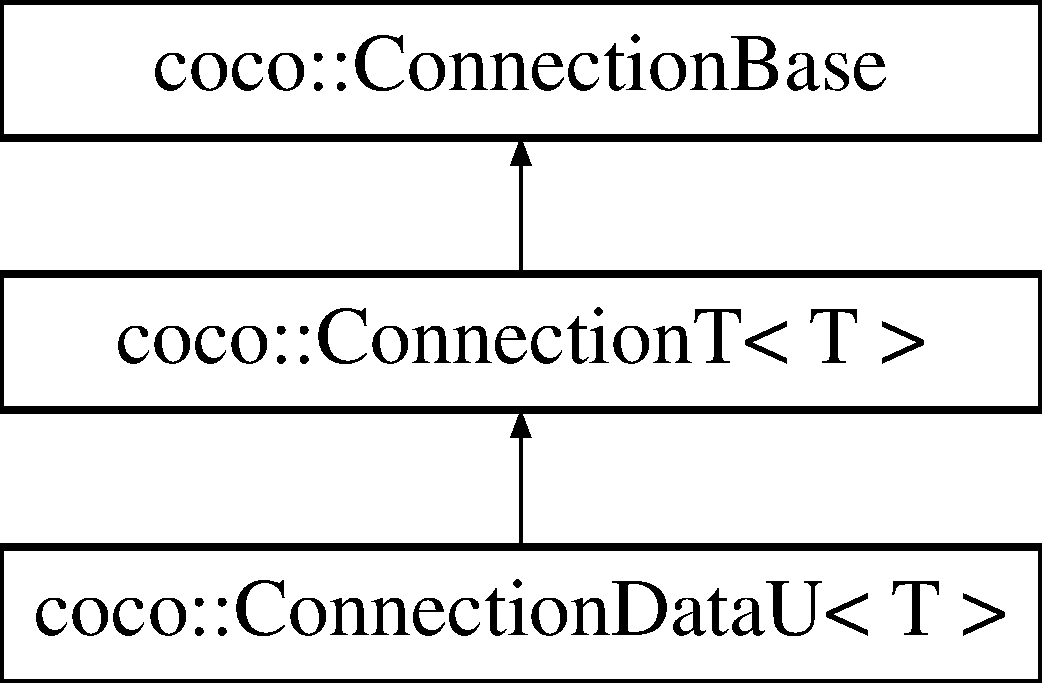
\includegraphics[height=3.000000cm]{classcoco_1_1_connection_data_u}
\end{center}
\end{figure}
\subsection*{Public Member Functions}
\begin{DoxyCompactItemize}
\item 
\hypertarget{classcoco_1_1_connection_data_u_aa5bf4219967a9deaa4d44aec278091d3}{\hyperlink{classcoco_1_1_connection_data_u_aa5bf4219967a9deaa4d44aec278091d3}{Connection\-Data\-U} (\hyperlink{classcoco_1_1_input_port}{Input\-Port}$<$ T $>$ $\ast$in, \hyperlink{classcoco_1_1_output_port}{Output\-Port}$<$ T $>$ $\ast$out, \hyperlink{structcoco_1_1_connection_policy}{Connection\-Policy} policy)}\label{classcoco_1_1_connection_data_u_aa5bf4219967a9deaa4d44aec278091d3}

\begin{DoxyCompactList}\small\item\em Simply call Connection\-T$<$\-T$>$ constructor. \end{DoxyCompactList}\item 
\hypertarget{classcoco_1_1_connection_data_u_aeef7e32d4fe7512b7ead3d3e069e0462}{virtual \hyperlink{namespacecoco_a057be58377e415c9be98c1dc5c8426ad}{Flow\-Status} \hyperlink{classcoco_1_1_connection_data_u_aeef7e32d4fe7512b7ead3d3e069e0462}{get\-Data} (T \&data) override}\label{classcoco_1_1_connection_data_u_aeef7e32d4fe7512b7ead3d3e069e0462}

\begin{DoxyCompactList}\small\item\em If there is new data in the container retrive it. \end{DoxyCompactList}\item 
\hypertarget{classcoco_1_1_connection_data_u_a886259fe50439a2dc9178cdf18178a42}{virtual bool \hyperlink{classcoco_1_1_connection_data_u_a886259fe50439a2dc9178cdf18178a42}{add\-Data} (T \&input) override}\label{classcoco_1_1_connection_data_u_a886259fe50439a2dc9178cdf18178a42}

\begin{DoxyCompactList}\small\item\em Add data to the container. If the input port is of type event trigger it to wake up the execution. \end{DoxyCompactList}\end{DoxyCompactItemize}
\subsection*{Private Attributes}
\begin{DoxyCompactItemize}
\item 
\hypertarget{classcoco_1_1_connection_data_u_a92f0caeeb4dfc2b9b9932a3a45d26f5a}{\begin{tabbing}
xx\=xx\=xx\=xx\=xx\=xx\=xx\=xx\=xx\=\kill
union \{\\
\>T {\bfseries value\_t\_}\\
\}; }\label{classcoco_1_1_connection_data_u_a92f0caeeb4dfc2b9b9932a3a45d26f5a}
\\

\end{tabbing}\end{DoxyCompactItemize}
\subsection*{Additional Inherited Members}


\subsection{Detailed Description}
\subsubsection*{template$<$class T$>$class coco\-::\-Connection\-Data\-U$<$ T $>$}

Specialized class for the type T to manage Connection\-Policy\-::\-D\-A\-T\-A Connection\-Policy\-::\-U\-N\-S\-Y\-N\-C. 

The documentation for this class was generated from the following file\-:\begin{DoxyCompactItemize}
\item 
src/ezoro.\-hpp\end{DoxyCompactItemize}

\hypertarget{classcoco_1_1_connection_manager}{\section{coco\-:\-:Connection\-Manager Class Reference}
\label{classcoco_1_1_connection_manager}\index{coco\-::\-Connection\-Manager@{coco\-::\-Connection\-Manager}}
}


Manage the connections of one \hyperlink{classcoco_1_1_port_base}{Port\-Base}.  




{\ttfamily \#include $<$ezoro.\-hpp$>$}

\subsection*{Public Member Functions}
\begin{DoxyCompactItemize}
\item 
\hypertarget{classcoco_1_1_connection_manager_acc77c57271baa8de5d3b20a10497a55d}{\hyperlink{classcoco_1_1_connection_manager_acc77c57271baa8de5d3b20a10497a55d}{Connection\-Manager} (\hyperlink{classcoco_1_1_port_base}{Port\-Base} $\ast$o)}\label{classcoco_1_1_connection_manager_acc77c57271baa8de5d3b20a10497a55d}

\begin{DoxyCompactList}\small\item\em set the Roun\-Robin index to 0 and set its \hyperlink{classcoco_1_1_port_base}{Port\-Base} ptr owner \end{DoxyCompactList}\item 
\hypertarget{classcoco_1_1_connection_manager_acc1eea2a62f85fb48aa3d7bce1e7e272}{bool \hyperlink{classcoco_1_1_connection_manager_acc1eea2a62f85fb48aa3d7bce1e7e272}{add\-Connection} (std\-::shared\-\_\-ptr$<$ \hyperlink{classcoco_1_1_connection_base}{Connection\-Base} $>$ connection)}\label{classcoco_1_1_connection_manager_acc1eea2a62f85fb48aa3d7bce1e7e272}

\begin{DoxyCompactList}\small\item\em add a connection to {\ttfamily connections\-\_\-} \end{DoxyCompactList}\item 
\hypertarget{classcoco_1_1_connection_manager_a81502d9aeb59d1c0b74d69e598f38d2b}{bool \hyperlink{classcoco_1_1_connection_manager_a81502d9aeb59d1c0b74d69e598f38d2b}{has\-Connections} () const }\label{classcoco_1_1_connection_manager_a81502d9aeb59d1c0b74d69e598f38d2b}

\begin{DoxyCompactList}\small\item\em return true if {\ttfamily connections\-\_\-} has at list one elemnt \end{DoxyCompactList}\item 
\hypertarget{classcoco_1_1_connection_manager_aa5765201013d82ff51e6b7d7f25202ea}{std\-::shared\-\_\-ptr$<$ \hyperlink{classcoco_1_1_connection_base}{Connection\-Base} $>$ \hyperlink{classcoco_1_1_connection_manager_aa5765201013d82ff51e6b7d7f25202ea}{get\-Connection} (int index)}\label{classcoco_1_1_connection_manager_aa5765201013d82ff51e6b7d7f25202ea}

\begin{DoxyCompactList}\small\item\em return the \hyperlink{classcoco_1_1_connection_base}{Connection\-Base} connection inidicated by index if it exist \end{DoxyCompactList}\item 
\hypertarget{classcoco_1_1_connection_manager_ae81d9b07af80bebc34b4472b221dea3e}{{\footnotesize template$<$class T $>$ }\\std\-::shared\-\_\-ptr$<$ \hyperlink{classcoco_1_1_connection_t}{Connection\-T}$<$ T $>$ $>$ \hyperlink{classcoco_1_1_connection_manager_ae81d9b07af80bebc34b4472b221dea3e}{get\-Connection\-T} (int index)}\label{classcoco_1_1_connection_manager_ae81d9b07af80bebc34b4472b221dea3e}

\begin{DoxyCompactList}\small\item\em return the Connection\-T$<$\-T$>$ connection inidicated by index if it exist \end{DoxyCompactList}\item 
\hypertarget{classcoco_1_1_connection_manager_aec1d76fc41d101b85442df22fcb6690b}{int \hyperlink{classcoco_1_1_connection_manager_aec1d76fc41d101b85442df22fcb6690b}{connections\-Size} () const }\label{classcoco_1_1_connection_manager_aec1d76fc41d101b85442df22fcb6690b}

\begin{DoxyCompactList}\small\item\em return the number of connections \end{DoxyCompactList}\end{DoxyCompactItemize}
\subsection*{Protected Attributes}
\begin{DoxyCompactItemize}
\item 
\hypertarget{classcoco_1_1_connection_manager_a96dd2c2e42aa9dd767746bb8e8771f2b}{int \hyperlink{classcoco_1_1_connection_manager_a96dd2c2e42aa9dd767746bb8e8771f2b}{rr\-\_\-index\-\_\-}}\label{classcoco_1_1_connection_manager_a96dd2c2e42aa9dd767746bb8e8771f2b}

\begin{DoxyCompactList}\small\item\em round robin index to poll the connection when reading data \end{DoxyCompactList}\item 
\hypertarget{classcoco_1_1_connection_manager_a620e2838da3375ebf9ecc6d0ef853e3d}{\hyperlink{classcoco_1_1_port_base}{Port\-Base} $\ast$ \hyperlink{classcoco_1_1_connection_manager_a620e2838da3375ebf9ecc6d0ef853e3d}{owner\-\_\-}}\label{classcoco_1_1_connection_manager_a620e2838da3375ebf9ecc6d0ef853e3d}

\begin{DoxyCompactList}\small\item\em \hyperlink{classcoco_1_1_port_base}{Port\-Base} pointer owning this manager. \end{DoxyCompactList}\item 
\hypertarget{classcoco_1_1_connection_manager_a1f34a36b21e6e124c3f954738f6717c4}{std\-::vector$<$ std\-::shared\-\_\-ptr\\*
$<$ \hyperlink{classcoco_1_1_connection_base}{Connection\-Base} $>$ $>$ \hyperlink{classcoco_1_1_connection_manager_a1f34a36b21e6e124c3f954738f6717c4}{connections\-\_\-}}\label{classcoco_1_1_connection_manager_a1f34a36b21e6e124c3f954738f6717c4}

\begin{DoxyCompactList}\small\item\em List of \hyperlink{classcoco_1_1_connection_base}{Connection\-Base} associate to {\ttfamily owner\-\_\-}. \end{DoxyCompactList}\end{DoxyCompactItemize}
\subsection*{Friends}
\begin{DoxyCompactItemize}
\item 
\hypertarget{classcoco_1_1_connection_manager_aa750daec74c1bf813c092ea268f3b8f8}{{\footnotesize template$<$class T $>$ }\\class {\bfseries Input\-Port}}\label{classcoco_1_1_connection_manager_aa750daec74c1bf813c092ea268f3b8f8}

\item 
\hypertarget{classcoco_1_1_connection_manager_a1b667fb33da7060c4747eeafcd85db20}{{\footnotesize template$<$class T $>$ }\\class {\bfseries Output\-Port}}\label{classcoco_1_1_connection_manager_a1b667fb33da7060c4747eeafcd85db20}

\end{DoxyCompactItemize}


\subsection{Detailed Description}
Manage the connections of one \hyperlink{classcoco_1_1_port_base}{Port\-Base}. 

Specialized class for the type T 

The documentation for this class was generated from the following file\-:\begin{DoxyCompactItemize}
\item 
src/ezoro.\-hpp\end{DoxyCompactItemize}

\hypertarget{structcoco_1_1_connection_policy}{\section{coco\-:\-:Connection\-Policy Struct Reference}
\label{structcoco_1_1_connection_policy}\index{coco\-::\-Connection\-Policy@{coco\-::\-Connection\-Policy}}
}


{\ttfamily \#include $<$ezoro.\-hpp$>$}

\subsection*{Public Types}
\begin{DoxyCompactItemize}
\item 
enum {\bfseries Policy} \{ {\bfseries D\-A\-T\-A}, 
{\bfseries B\-U\-F\-F\-E\-R}, 
{\bfseries C\-I\-R\-C\-U\-L\-A\-R}
 \}
\item 
enum {\bfseries Lock\-Policy} \{ {\bfseries U\-N\-S\-Y\-N\-C}, 
{\bfseries L\-O\-C\-K\-E\-D}, 
{\bfseries L\-O\-C\-K\-\_\-\-F\-R\-E\-E}
 \}
\item 
enum {\bfseries Transport} \{ {\bfseries L\-O\-C\-A\-L}, 
{\bfseries I\-P\-C}
 \}
\end{DoxyCompactItemize}
\subsection*{Public Member Functions}
\begin{DoxyCompactItemize}
\item 
\hyperlink{structcoco_1_1_connection_policy_a4f57d8138b054a591016a35fc4aa6bea}{Connection\-Policy} ()
\item 
\hypertarget{structcoco_1_1_connection_policy_a70af7262ac5e18bbeb38fc5b5b1459aa}{{\bfseries Connection\-Policy} (Policy policiy, int buffer\-\_\-size, bool blocking=false)}\label{structcoco_1_1_connection_policy_a70af7262ac5e18bbeb38fc5b5b1459aa}

\end{DoxyCompactItemize}
\subsection*{Public Attributes}
\begin{DoxyCompactItemize}
\item 
Policy \hyperlink{structcoco_1_1_connection_policy_aa37517fcc9cd9bfd6d3922023b16a488}{data\-\_\-policy\-\_\-}
\item 
\hypertarget{structcoco_1_1_connection_policy_acaa6623737829cb63001a7266795dfcd}{Lock\-Policy {\bfseries lock\-\_\-policy\-\_\-}}\label{structcoco_1_1_connection_policy_acaa6623737829cb63001a7266795dfcd}

\item 
int \hyperlink{structcoco_1_1_connection_policy_a481122e34e02c0bce981ea65c2a10b0c}{buffer\-\_\-size\-\_\-}
\item 
bool \hyperlink{structcoco_1_1_connection_policy_a359054d26257b4e074d69b943d8453e8}{init\-\_\-}
\item 
\hypertarget{structcoco_1_1_connection_policy_a1ff94843c53e3abc8c246cbb16dc72d3}{std\-::string {\bfseries name\-\_\-id\-\_\-}}\label{structcoco_1_1_connection_policy_a1ff94843c53e3abc8c246cbb16dc72d3}

\item 
\hypertarget{structcoco_1_1_connection_policy_ac33574e0a7670ea03848d34726e67728}{Transport {\bfseries transport\-\_\-} = L\-O\-C\-A\-L}\label{structcoco_1_1_connection_policy_ac33574e0a7670ea03848d34726e67728}

\end{DoxyCompactItemize}


\subsection{Detailed Description}
Connection Policy 

\subsection{Constructor \& Destructor Documentation}
\hypertarget{structcoco_1_1_connection_policy_a4f57d8138b054a591016a35fc4aa6bea}{\index{coco\-::\-Connection\-Policy@{coco\-::\-Connection\-Policy}!Connection\-Policy@{Connection\-Policy}}
\index{Connection\-Policy@{Connection\-Policy}!coco::ConnectionPolicy@{coco\-::\-Connection\-Policy}}
\subsubsection[{Connection\-Policy}]{\setlength{\rightskip}{0pt plus 5cm}coco\-::\-Connection\-Policy\-::\-Connection\-Policy (
\begin{DoxyParamCaption}
{}
\end{DoxyParamCaption}
)\hspace{0.3cm}{\ttfamily [inline]}}}\label{structcoco_1_1_connection_policy_a4f57d8138b054a591016a35fc4aa6bea}
Default constructor, default value\-: 
\begin{DoxyParams}{Parameters}
{\em data\-\_\-policy\-\_\-} & = D\-A\-T\-A \\
\hline
{\em lock\-\_\-policy\-\_\-} & = L\-O\-C\-K\-E\-D \\
\hline
{\em buffer\-\_\-size\-\_\-} & = 1 \\
\hline
{\em init\-\_\-} & = 1 \\
\hline
\end{DoxyParams}


\subsection{Member Data Documentation}
\hypertarget{structcoco_1_1_connection_policy_a481122e34e02c0bce981ea65c2a10b0c}{\index{coco\-::\-Connection\-Policy@{coco\-::\-Connection\-Policy}!buffer\-\_\-size\-\_\-@{buffer\-\_\-size\-\_\-}}
\index{buffer\-\_\-size\-\_\-@{buffer\-\_\-size\-\_\-}!coco::ConnectionPolicy@{coco\-::\-Connection\-Policy}}
\subsubsection[{buffer\-\_\-size\-\_\-}]{\setlength{\rightskip}{0pt plus 5cm}int coco\-::\-Connection\-Policy\-::buffer\-\_\-size\-\_\-}}\label{structcoco_1_1_connection_policy_a481122e34e02c0bce981ea65c2a10b0c}
type of lock policy 

Referenced by coco\-::\-Connection\-Buffer\-L$<$ T $>$\-::\-Connection\-Buffer\-L(), coco\-::\-Connection\-Buffer\-U$<$ T $>$\-::\-Connection\-Buffer\-U(), and coco\-::make\-Connection().

\hypertarget{structcoco_1_1_connection_policy_aa37517fcc9cd9bfd6d3922023b16a488}{\index{coco\-::\-Connection\-Policy@{coco\-::\-Connection\-Policy}!data\-\_\-policy\-\_\-@{data\-\_\-policy\-\_\-}}
\index{data\-\_\-policy\-\_\-@{data\-\_\-policy\-\_\-}!coco::ConnectionPolicy@{coco\-::\-Connection\-Policy}}
\subsubsection[{data\-\_\-policy\-\_\-}]{\setlength{\rightskip}{0pt plus 5cm}Policy coco\-::\-Connection\-Policy\-::data\-\_\-policy\-\_\-}}\label{structcoco_1_1_connection_policy_aa37517fcc9cd9bfd6d3922023b16a488}
type of data container 

Referenced by coco\-::\-Connection\-Buffer\-U$<$ T $>$\-::add\-Data(), coco\-::\-Connection\-Buffer\-L$<$ T $>$\-::add\-Data(), and coco\-::make\-Connection().

\hypertarget{structcoco_1_1_connection_policy_a359054d26257b4e074d69b943d8453e8}{\index{coco\-::\-Connection\-Policy@{coco\-::\-Connection\-Policy}!init\-\_\-@{init\-\_\-}}
\index{init\-\_\-@{init\-\_\-}!coco::ConnectionPolicy@{coco\-::\-Connection\-Policy}}
\subsubsection[{init\-\_\-}]{\setlength{\rightskip}{0pt plus 5cm}bool coco\-::\-Connection\-Policy\-::init\-\_\-}}\label{structcoco_1_1_connection_policy_a359054d26257b4e074d69b943d8453e8}
size of the data container 

The documentation for this struct was generated from the following file\-:\begin{DoxyCompactItemize}
\item 
src/ezoro.\-hpp\end{DoxyCompactItemize}

\hypertarget{classcoco_1_1_connection_t}{}\section{coco\+:\+:Connection\+T$<$ T $>$ Class Template Reference}
\label{classcoco_1_1_connection_t}\index{coco\+::\+Connection\+T$<$ T $>$@{coco\+::\+Connection\+T$<$ T $>$}}


Template class to manage the type of the connection.  




{\ttfamily \#include $<$coco\+\_\+core.\+hpp$>$}

Inheritance diagram for coco\+:\+:Connection\+T$<$ T $>$\+:\begin{figure}[H]
\begin{center}
\leavevmode
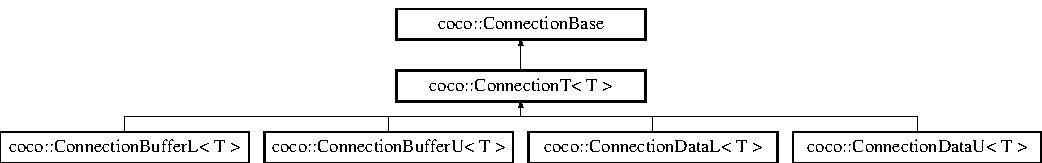
\includegraphics[height=2.187500cm]{classcoco_1_1_connection_t}
\end{center}
\end{figure}
\subsection*{Public Member Functions}
\begin{DoxyCompactItemize}
\item 
\hypertarget{classcoco_1_1_connection_t_a036f8c67d029ce417a331df695d49515}{}\hyperlink{classcoco_1_1_connection_t_a036f8c67d029ce417a331df695d49515}{Connection\+T} (\hyperlink{classcoco_1_1_input_port}{Input\+Port}$<$ T $>$ $\ast$in, \hyperlink{classcoco_1_1_output_port}{Output\+Port}$<$ T $>$ $\ast$out, \hyperlink{structcoco_1_1_connection_policy}{Connection\+Policy} policy)\label{classcoco_1_1_connection_t_a036f8c67d029ce417a331df695d49515}

\begin{DoxyCompactList}\small\item\em Simply call \hyperlink{classcoco_1_1_connection_base}{Connection\+Base} constructor. \end{DoxyCompactList}\item 
\hypertarget{classcoco_1_1_connection_t_aed88cfa8b0384f879b09561096b35a56}{}virtual \hyperlink{namespacecoco_a057be58377e415c9be98c1dc5c8426ad}{Flow\+Status} \hyperlink{classcoco_1_1_connection_t_aed88cfa8b0384f879b09561096b35a56}{get\+Data} (T \&data)=0\label{classcoco_1_1_connection_t_aed88cfa8b0384f879b09561096b35a56}

\begin{DoxyCompactList}\small\item\em If there is new data in the container retrive it. \end{DoxyCompactList}\item 
\hypertarget{classcoco_1_1_connection_t_addca57488f686446a10e0f37bfa8c1ea}{}virtual bool \hyperlink{classcoco_1_1_connection_t_addca57488f686446a10e0f37bfa8c1ea}{add\+Data} (T \&data)=0\label{classcoco_1_1_connection_t_addca57488f686446a10e0f37bfa8c1ea}

\begin{DoxyCompactList}\small\item\em Add data to the container. ~\newline
 If the input port is of type event trigger it to wake up the execution. \end{DoxyCompactList}\end{DoxyCompactItemize}
\subsection*{Additional Inherited Members}


\subsection{Detailed Description}
\subsubsection*{template$<$class T$>$class coco\+::\+Connection\+T$<$ T $>$}

Template class to manage the type of the connection. 

The documentation for this class was generated from the following file\+:\begin{DoxyCompactItemize}
\item 
src/coco\+\_\+core.\+hpp\end{DoxyCompactItemize}

\hypertarget{classcoco_1_1_execution_engine}{}\section{coco\+:\+:Execution\+Engine Class Reference}
\label{classcoco_1_1_execution_engine}\index{coco\+::\+Execution\+Engine@{coco\+::\+Execution\+Engine}}


Concrete class to execture the components.  




{\ttfamily \#include $<$coco\+\_\+core.\+hpp$>$}

Inheritance diagram for coco\+:\+:Execution\+Engine\+:\begin{figure}[H]
\begin{center}
\leavevmode
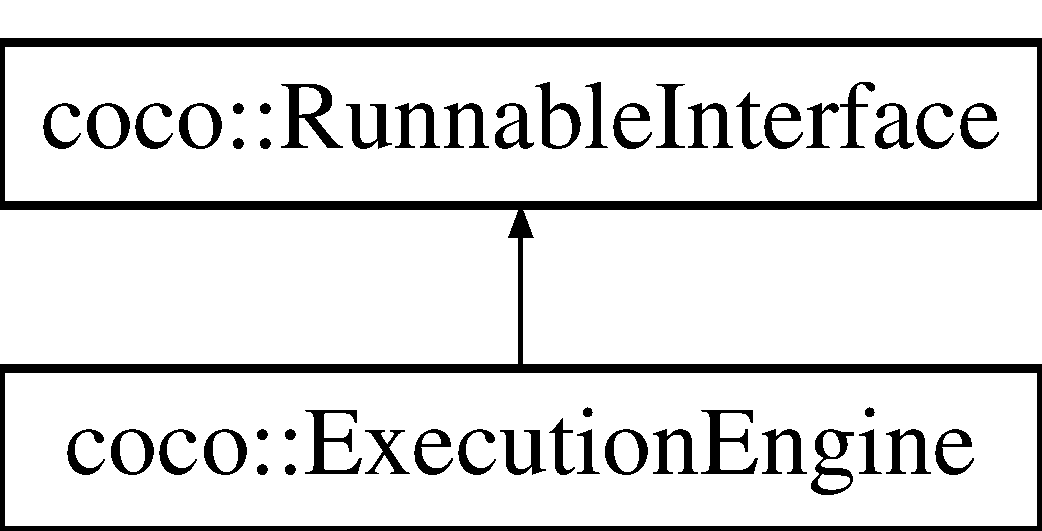
\includegraphics[height=2.000000cm]{classcoco_1_1_execution_engine}
\end{center}
\end{figure}
\subsection*{Public Member Functions}
\begin{DoxyCompactItemize}
\item 
\hypertarget{classcoco_1_1_execution_engine_aa0a33c45c90946986237b0ccc82338ce}{}\hyperlink{classcoco_1_1_execution_engine_aa0a33c45c90946986237b0ccc82338ce}{Execution\+Engine} (\hyperlink{classcoco_1_1_task_context}{Task\+Context} $\ast$t)\label{classcoco_1_1_execution_engine_aa0a33c45c90946986237b0ccc82338ce}

\begin{DoxyCompactList}\small\item\em Constructor to set the current \hyperlink{classcoco_1_1_task_context}{Task\+Context} to be executed. \end{DoxyCompactList}\item 
\hypertarget{classcoco_1_1_execution_engine_a99ee8574a588ae8fa647bbca9f314fbd}{}virtual void \hyperlink{classcoco_1_1_execution_engine_a99ee8574a588ae8fa647bbca9f314fbd}{init} () override\label{classcoco_1_1_execution_engine_a99ee8574a588ae8fa647bbca9f314fbd}

\begin{DoxyCompactList}\small\item\em Initialize the components members. \end{DoxyCompactList}\item 
\hypertarget{classcoco_1_1_execution_engine_a9c3cfba8051944ac90a12bae7baf99c3}{}virtual void \hyperlink{classcoco_1_1_execution_engine_a9c3cfba8051944ac90a12bae7baf99c3}{step} () override\label{classcoco_1_1_execution_engine_a9c3cfba8051944ac90a12bae7baf99c3}

\begin{DoxyCompactList}\small\item\em If the task is running execute uno step of the execution function. \end{DoxyCompactList}\item 
\hypertarget{classcoco_1_1_execution_engine_a5375d0bb4a83c1c4142ea9907220c4c7}{}virtual void \hyperlink{classcoco_1_1_execution_engine_a5375d0bb4a83c1c4142ea9907220c4c7}{finalize} () override\label{classcoco_1_1_execution_engine_a5375d0bb4a83c1c4142ea9907220c4c7}

\begin{DoxyCompactList}\small\item\em When the task is stopped clear all the members. \end{DoxyCompactList}\end{DoxyCompactItemize}
\subsection*{Protected Attributes}
\begin{DoxyCompactItemize}
\item 
\hypertarget{classcoco_1_1_execution_engine_ae0729158d86ae748445f521baea61d7a}{}\hyperlink{classcoco_1_1_task_context}{Task\+Context} $\ast$ {\bfseries task\+\_\+}\label{classcoco_1_1_execution_engine_ae0729158d86ae748445f521baea61d7a}

\item 
\hypertarget{classcoco_1_1_execution_engine_a5a3c72d66f0395812ca730c826690a66}{}bool {\bfseries stopped\+\_\+}\label{classcoco_1_1_execution_engine_a5a3c72d66f0395812ca730c826690a66}

\end{DoxyCompactItemize}


\subsection{Detailed Description}
Concrete class to execture the components. 

The documentation for this class was generated from the following files\+:\begin{DoxyCompactItemize}
\item 
src/coco\+\_\+core.\+hpp\item 
src/coco\+\_\+core.\+cpp\end{DoxyCompactItemize}

\hypertarget{structcoco_1_1impl_1_1getfunctioner}{}\section{coco\+:\+:impl\+:\+:getfunctioner$<$ T $>$ Struct Template Reference}
\label{structcoco_1_1impl_1_1getfunctioner}\index{coco\+::impl\+::getfunctioner$<$ T $>$@{coco\+::impl\+::getfunctioner$<$ T $>$}}


The documentation for this struct was generated from the following file\+:\begin{DoxyCompactItemize}
\item 
src/coco\+\_\+core.\+hpp\end{DoxyCompactItemize}

\hypertarget{structcoco_1_1impl_1_1getfunctioner_3_01_r_07_args_8_8_8_08_4}{}\section{coco\+:\+:impl\+:\+:getfunctioner$<$ R(Args...)$>$ Struct Template Reference}
\label{structcoco_1_1impl_1_1getfunctioner_3_01_r_07_args_8_8_8_08_4}\index{coco\+::impl\+::getfunctioner$<$ R(\+Args...)$>$@{coco\+::impl\+::getfunctioner$<$ R(\+Args...)$>$}}
\subsection*{Public Types}
\begin{DoxyCompactItemize}
\item 
\hypertarget{structcoco_1_1impl_1_1getfunctioner_3_01_r_07_args_8_8_8_08_4_a7572e5f95c6cb289a8ff1ebbd5aaa8a7}{}typedef std\+::function$<$ R(Args...)$>$ {\bfseries target}\label{structcoco_1_1impl_1_1getfunctioner_3_01_r_07_args_8_8_8_08_4_a7572e5f95c6cb289a8ff1ebbd5aaa8a7}

\item 
\hypertarget{structcoco_1_1impl_1_1getfunctioner_3_01_r_07_args_8_8_8_08_4_af21388293087ebe0cdffbee090673e81}{}using {\bfseries fx} = R(Args...)\label{structcoco_1_1impl_1_1getfunctioner_3_01_r_07_args_8_8_8_08_4_af21388293087ebe0cdffbee090673e81}

\end{DoxyCompactItemize}


The documentation for this struct was generated from the following file\+:\begin{DoxyCompactItemize}
\item 
src/coco\+\_\+core.\+hpp\end{DoxyCompactItemize}

\hypertarget{structcoco_1_1impl_1_1getfunctioner_3_01_r_07_u_1_1_5_08_07_args_8_8_8_08_01_4}{}\section{coco\+:\+:impl\+:\+:getfunctioner$<$ R(U\+:\+:$\ast$)(Args...) $>$ Struct Template Reference}
\label{structcoco_1_1impl_1_1getfunctioner_3_01_r_07_u_1_1_5_08_07_args_8_8_8_08_01_4}\index{coco\+::impl\+::getfunctioner$<$ R(\+U\+::$\ast$)(\+Args...) $>$@{coco\+::impl\+::getfunctioner$<$ R(\+U\+::$\ast$)(\+Args...) $>$}}
\subsection*{Public Types}
\begin{DoxyCompactItemize}
\item 
\hypertarget{structcoco_1_1impl_1_1getfunctioner_3_01_r_07_u_1_1_5_08_07_args_8_8_8_08_01_4_aef261d7a62b54d064177787cff33336f}{}typedef std\+::function$<$ R(Args...)$>$ {\bfseries target}\label{structcoco_1_1impl_1_1getfunctioner_3_01_r_07_u_1_1_5_08_07_args_8_8_8_08_01_4_aef261d7a62b54d064177787cff33336f}

\item 
\hypertarget{structcoco_1_1impl_1_1getfunctioner_3_01_r_07_u_1_1_5_08_07_args_8_8_8_08_01_4_a2490959e1992e8ec9903d0ec253c7cfc}{}using {\bfseries fx} = R(Args...)\label{structcoco_1_1impl_1_1getfunctioner_3_01_r_07_u_1_1_5_08_07_args_8_8_8_08_01_4_a2490959e1992e8ec9903d0ec253c7cfc}

\end{DoxyCompactItemize}


The documentation for this struct was generated from the following file\+:\begin{DoxyCompactItemize}
\item 
src/coco\+\_\+core.\+hpp\end{DoxyCompactItemize}

\hypertarget{structcoco_1_1impl_1_1getfunctioner_3_01std_1_1function_3_01_r_07_args_8_8_8_08_01_4_01_4}{\section{coco\-:\-:impl\-:\-:getfunctioner$<$ std\-:\-:function$<$ R(Args...) $>$ $>$ Struct Template Reference}
\label{structcoco_1_1impl_1_1getfunctioner_3_01std_1_1function_3_01_r_07_args_8_8_8_08_01_4_01_4}\index{coco\-::impl\-::getfunctioner$<$ std\-::function$<$ R(\-Args...) $>$ $>$@{coco\-::impl\-::getfunctioner$<$ std\-::function$<$ R(\-Args...) $>$ $>$}}
}
\subsection*{Public Types}
\begin{DoxyCompactItemize}
\item 
\hypertarget{structcoco_1_1impl_1_1getfunctioner_3_01std_1_1function_3_01_r_07_args_8_8_8_08_01_4_01_4_a8a0ab3a18eea8ead50fed7ac6e9670b2}{typedef std\-::function$<$ R(Args...)$>$ {\bfseries target}}\label{structcoco_1_1impl_1_1getfunctioner_3_01std_1_1function_3_01_r_07_args_8_8_8_08_01_4_01_4_a8a0ab3a18eea8ead50fed7ac6e9670b2}

\item 
\hypertarget{structcoco_1_1impl_1_1getfunctioner_3_01std_1_1function_3_01_r_07_args_8_8_8_08_01_4_01_4_a4473bf83da1d20b603ae38bf5b6e1977}{using {\bfseries fx} = R(Args...)}\label{structcoco_1_1impl_1_1getfunctioner_3_01std_1_1function_3_01_r_07_args_8_8_8_08_01_4_01_4_a4473bf83da1d20b603ae38bf5b6e1977}

\end{DoxyCompactItemize}


The documentation for this struct was generated from the following file\-:\begin{DoxyCompactItemize}
\item 
src/ezoro.\-hpp\end{DoxyCompactItemize}

\hypertarget{classcoco_1_1_input_port}{}\section{coco\+:\+:Input\+Port$<$ T $>$ Class Template Reference}
\label{classcoco_1_1_input_port}\index{coco\+::\+Input\+Port$<$ T $>$@{coco\+::\+Input\+Port$<$ T $>$}}


Class representing an input port containing data of type T.  




{\ttfamily \#include $<$coco\+\_\+core.\+hpp$>$}

Inheritance diagram for coco\+:\+:Input\+Port$<$ T $>$\+:\begin{figure}[H]
\begin{center}
\leavevmode
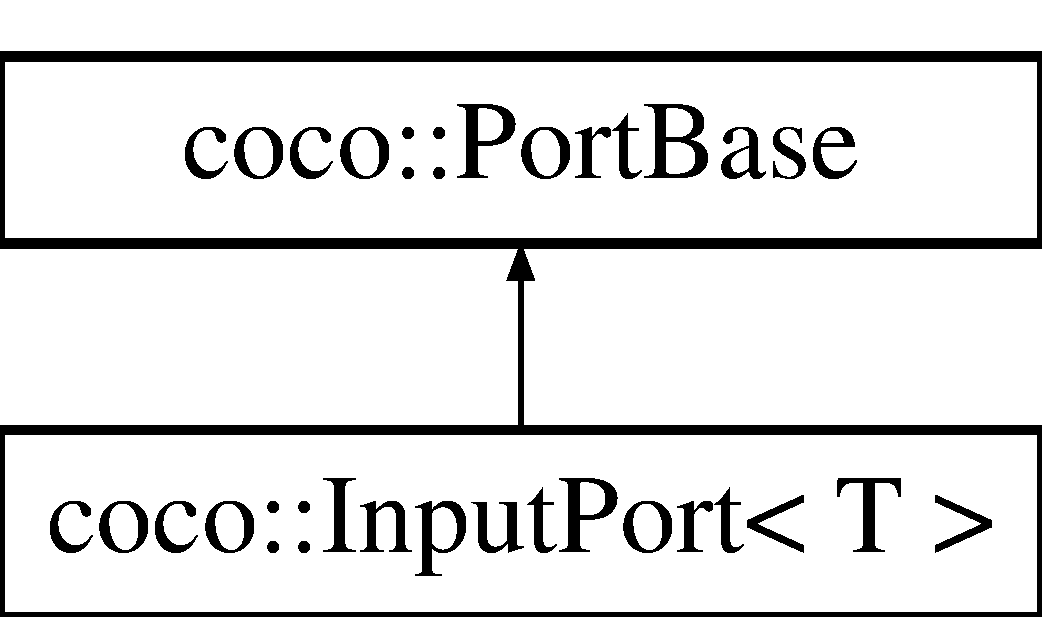
\includegraphics[height=2.000000cm]{classcoco_1_1_input_port}
\end{center}
\end{figure}
\subsection*{Public Member Functions}
\begin{DoxyCompactItemize}
\item 
\hypertarget{classcoco_1_1_input_port_a30034afe3a136863e24e37cf7bd18a48}{}\hyperlink{classcoco_1_1_input_port_a30034afe3a136863e24e37cf7bd18a48}{Input\+Port} (\hyperlink{classcoco_1_1_task_context}{Task\+Context} $\ast$p, const std\+::string \&\hyperlink{classcoco_1_1_port_base_abf4eb7fcc3ec9973ee73dd140e7646db}{name}, bool is\+\_\+event=false)\label{classcoco_1_1_input_port_a30034afe3a136863e24e37cf7bd18a48}

\begin{DoxyCompactList}\small\item\em Simply call \hyperlink{classcoco_1_1_port_base}{Port\+Base} constructor. \end{DoxyCompactList}\item 
\hypertarget{classcoco_1_1_input_port_a6b0d4b4de9199a102168c767756d0000}{}const std\+::type\+\_\+info \& \hyperlink{classcoco_1_1_input_port_a6b0d4b4de9199a102168c767756d0000}{get\+Type\+Info} () const override\label{classcoco_1_1_input_port_a6b0d4b4de9199a102168c767756d0000}

\begin{DoxyCompactList}\small\item\em Get the type of the Port variable. \end{DoxyCompactList}\item 
\hypertarget{classcoco_1_1_input_port_a838df83833fa100b992eb96c5cc01536}{}bool \hyperlink{classcoco_1_1_input_port_a838df83833fa100b992eb96c5cc01536}{connect\+To} (\hyperlink{classcoco_1_1_port_base}{Port\+Base} $\ast$other, \hyperlink{structcoco_1_1_connection_policy}{Connection\+Policy} policy)\label{classcoco_1_1_input_port_a838df83833fa100b992eb96c5cc01536}

\begin{DoxyCompactList}\small\item\em Connect this port to an \hyperlink{classcoco_1_1_output_port}{Output\+Port}. \end{DoxyCompactList}\item 
\hypertarget{classcoco_1_1_input_port_a92e1dd40c0f20d207c7098ba9699c89f}{}\hyperlink{namespacecoco_a057be58377e415c9be98c1dc5c8426ad}{Flow\+Status} \hyperlink{classcoco_1_1_input_port_a92e1dd40c0f20d207c7098ba9699c89f}{read} (T \&output)\label{classcoco_1_1_input_port_a92e1dd40c0f20d207c7098ba9699c89f}

\begin{DoxyCompactList}\small\item\em Using a round robin schedule polls all its connections to see if someone has new data to be read. \end{DoxyCompactList}\item 
\hyperlink{namespacecoco_a057be58377e415c9be98c1dc5c8426ad}{Flow\+Status} \hyperlink{classcoco_1_1_input_port_a0936ee02f6f53d6ba6e379477f5e223b}{read\+All} (std\+::vector$<$ T $>$ \&output)
\end{DoxyCompactItemize}
\subsection*{Private Member Functions}
\begin{DoxyCompactItemize}
\item 
\hypertarget{classcoco_1_1_input_port_a4182500b2ff28fa95628d645f18ba457}{}std\+::shared\+\_\+ptr$<$ \hyperlink{classcoco_1_1_connection_t}{Connection\+T}$<$ T $>$ $>$ \hyperlink{classcoco_1_1_input_port_a4182500b2ff28fa95628d645f18ba457}{get\+Connection} (int index)\label{classcoco_1_1_input_port_a4182500b2ff28fa95628d645f18ba457}

\begin{DoxyCompactList}\small\item\em Get the connection at position {\ttfamily index}. \end{DoxyCompactList}\item 
\hypertarget{classcoco_1_1_input_port_aff01c8e8366eb6b7b5911fd10a6acc00}{}bool \hyperlink{classcoco_1_1_input_port_aff01c8e8366eb6b7b5911fd10a6acc00}{connect\+To\+Typed} (\hyperlink{classcoco_1_1_output_port}{Output\+Port}$<$ T $>$ $\ast$other, \hyperlink{structcoco_1_1_connection_policy}{Connection\+Policy} policy)\label{classcoco_1_1_input_port_aff01c8e8366eb6b7b5911fd10a6acc00}

\begin{DoxyCompactList}\small\item\em Connect the current port with {\ttfamily other},. \end{DoxyCompactList}\end{DoxyCompactItemize}
\subsection*{Additional Inherited Members}


\subsection{Detailed Description}
\subsubsection*{template$<$class T$>$class coco\+::\+Input\+Port$<$ T $>$}

Class representing an input port containing data of type T. 

\subsection{Member Function Documentation}
\hypertarget{classcoco_1_1_input_port_a0936ee02f6f53d6ba6e379477f5e223b}{}\index{coco\+::\+Input\+Port@{coco\+::\+Input\+Port}!read\+All@{read\+All}}
\index{read\+All@{read\+All}!coco\+::\+Input\+Port@{coco\+::\+Input\+Port}}
\subsubsection[{read\+All}]{\setlength{\rightskip}{0pt plus 5cm}template$<$class T$>$ {\bf Flow\+Status} {\bf coco\+::\+Input\+Port}$<$ T $>$\+::read\+All (
\begin{DoxyParamCaption}
\item[{std\+::vector$<$ T $>$ \&}]{output}
\end{DoxyParamCaption}
)\hspace{0.3cm}{\ttfamily [inline]}}\label{classcoco_1_1_input_port_a0936ee02f6f53d6ba6e379477f5e223b}
Using a round robin schedule polls all its connections to see if someone has new data to be read If a connection is a buffer read all data in the buffer! 

References coco\+::\+Port\+Base\+::connections\+Count(), and coco\+::\+Input\+Port$<$ T $>$\+::get\+Connection().



The documentation for this class was generated from the following file\+:\begin{DoxyCompactItemize}
\item 
src/coco\+\_\+core.\+hpp\end{DoxyCompactItemize}

\hypertarget{structcoco_1_1impl_1_1int__sequence}{}\section{coco\+:\+:impl\+:\+:int\+\_\+sequence$<$$>$ Struct Template Reference}
\label{structcoco_1_1impl_1_1int__sequence}\index{coco\+::impl\+::int\+\_\+sequence$<$$>$@{coco\+::impl\+::int\+\_\+sequence$<$$>$}}


The documentation for this struct was generated from the following file\+:\begin{DoxyCompactItemize}
\item 
src/coco\+\_\+core.\+hpp\end{DoxyCompactItemize}

\hypertarget{structstd_1_1is__placeholder_3_01placeholder__template_3_01_n_01_4_01_4}{}\section{std\+:\+:is\+\_\+placeholder$<$ placeholder\+\_\+template$<$ N $>$ $>$ Struct Template Reference}
\label{structstd_1_1is__placeholder_3_01placeholder__template_3_01_n_01_4_01_4}\index{std\+::is\+\_\+placeholder$<$ placeholder\+\_\+template$<$ N $>$ $>$@{std\+::is\+\_\+placeholder$<$ placeholder\+\_\+template$<$ N $>$ $>$}}
Inheritance diagram for std\+:\+:is\+\_\+placeholder$<$ placeholder\+\_\+template$<$ N $>$ $>$\+:\begin{figure}[H]
\begin{center}
\leavevmode
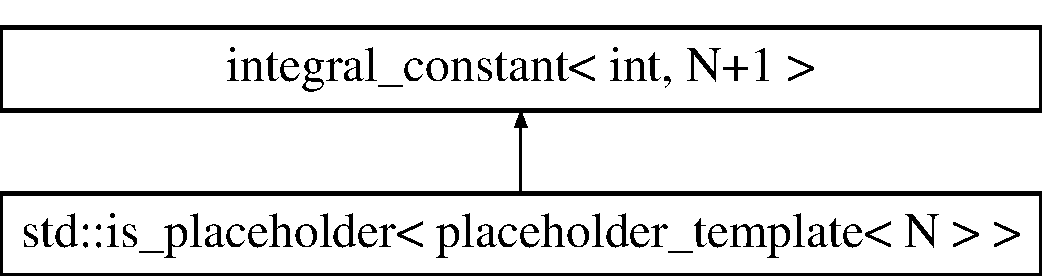
\includegraphics[height=2.000000cm]{structstd_1_1is__placeholder_3_01placeholder__template_3_01_n_01_4_01_4}
\end{center}
\end{figure}


The documentation for this struct was generated from the following file\+:\begin{DoxyCompactItemize}
\item 
src/coco\+\_\+impl.\+hpp\end{DoxyCompactItemize}

\input{structcoco_1_1impl_1_1mapkeys__t_1_1iterator}
\input{structcoco_1_1impl_1_1mapvalues__t_1_1iterator}
\input{classcoco_1_1_logger_manager}
\input{classcoco_1_1_log_message}
\input{classcoco_1_1_log_message_sampled}
\hypertarget{structcoco_1_1impl_1_1make__int__sequence}{}\section{coco\+:\+:impl\+:\+:make\+\_\+int\+\_\+sequence$<$ N, Is $>$ Struct Template Reference}
\label{structcoco_1_1impl_1_1make__int__sequence}\index{coco\+::impl\+::make\+\_\+int\+\_\+sequence$<$ N, Is $>$@{coco\+::impl\+::make\+\_\+int\+\_\+sequence$<$ N, Is $>$}}


The documentation for this struct was generated from the following file\+:\begin{DoxyCompactItemize}
\item 
src/coco\+\_\+impl.\+hpp\end{DoxyCompactItemize}

\hypertarget{structcoco_1_1impl_1_1make__int__sequence_3_010_00_01_is_8_8_8_4}{}\section{coco\+:\+:impl\+:\+:make\+\_\+int\+\_\+sequence$<$ 0, Is...$>$ Struct Template Reference}
\label{structcoco_1_1impl_1_1make__int__sequence_3_010_00_01_is_8_8_8_4}\index{coco\+::impl\+::make\+\_\+int\+\_\+sequence$<$ 0, Is...$>$@{coco\+::impl\+::make\+\_\+int\+\_\+sequence$<$ 0, Is...$>$}}
Inheritance diagram for coco\+:\+:impl\+:\+:make\+\_\+int\+\_\+sequence$<$ 0, Is...$>$\+:\begin{figure}[H]
\begin{center}
\leavevmode
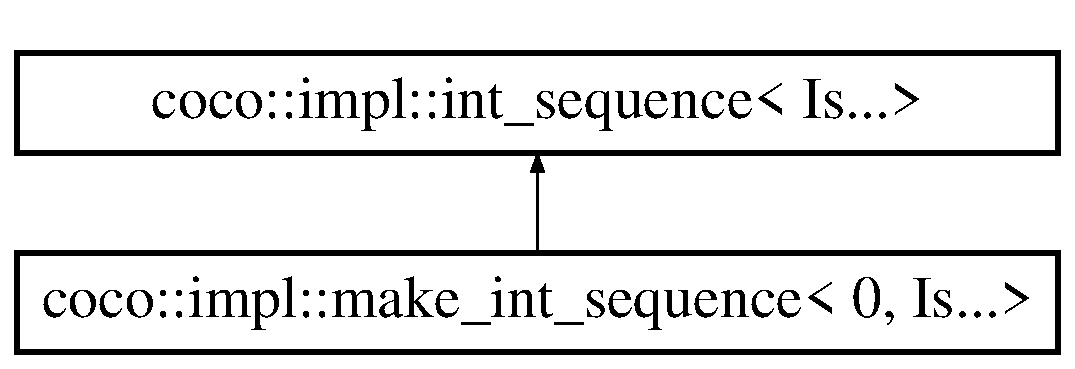
\includegraphics[height=2.000000cm]{structcoco_1_1impl_1_1make__int__sequence_3_010_00_01_is_8_8_8_4}
\end{center}
\end{figure}


The documentation for this struct was generated from the following file\+:\begin{DoxyCompactItemize}
\item 
src/coco\+\_\+core.\+hpp\end{DoxyCompactItemize}

\input{structcoco_1_1_make_connection__t}
\input{structcoco_1_1impl_1_1mapkeys__t}
\input{structcoco_1_1impl_1_1mapvalues__t}
\hypertarget{classcoco_1_1_operation}{}\section{coco\+:\+:Operation$<$ T $>$ Class Template Reference}
\label{classcoco_1_1_operation}\index{coco\+::\+Operation$<$ T $>$@{coco\+::\+Operation$<$ T $>$}}


{\ttfamily \#include $<$coco\+\_\+core.\+hpp$>$}

Inheritance diagram for coco\+:\+:Operation$<$ T $>$\+:\begin{figure}[H]
\begin{center}
\leavevmode
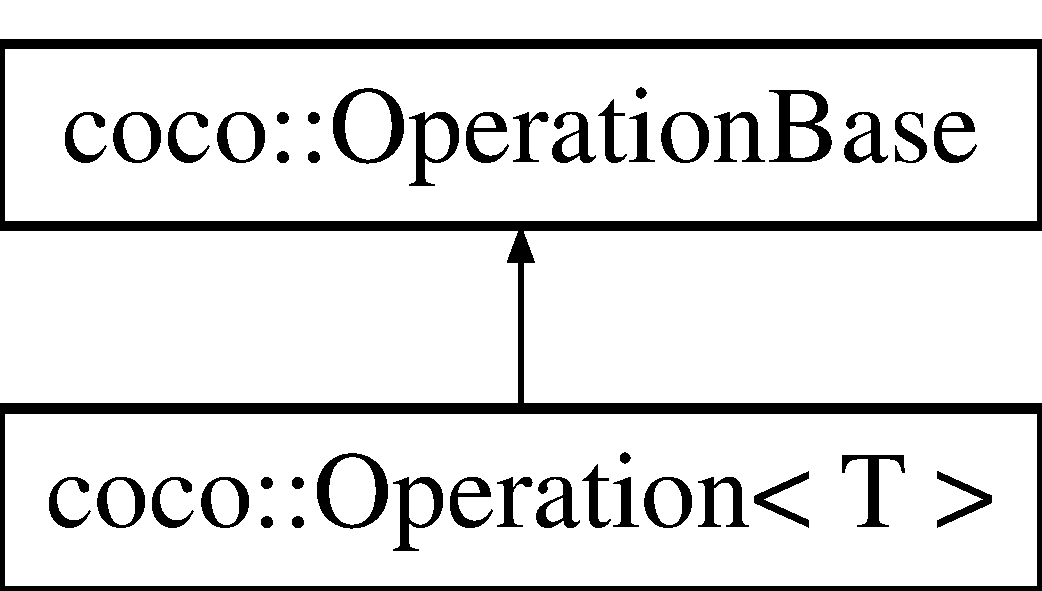
\includegraphics[height=2.000000cm]{classcoco_1_1_operation}
\end{center}
\end{figure}
\subsection*{Public Types}
\begin{DoxyCompactItemize}
\item 
\hypertarget{classcoco_1_1_operation_a0ca4f6e3d30de1c5121d5b55f7abb5ac}{}typedef \hyperlink{structcoco_1_1impl_1_1get__functioner}{coco\+::impl\+::get\+\_\+functioner}$<$ T $>$\+::fx {\bfseries Sig}\label{classcoco_1_1_operation_a0ca4f6e3d30de1c5121d5b55f7abb5ac}

\end{DoxyCompactItemize}
\subsection*{Public Member Functions}
\begin{DoxyCompactItemize}
\item 
\hypertarget{classcoco_1_1_operation_a4480feab07c13ab9948fa19bd13ca9a4}{}{\bfseries Operation} (\hyperlink{classcoco_1_1_service}{Service} $\ast$p, const std\+::string \&\hyperlink{classcoco_1_1_operation_base_aee0ff9e503d67abe3260e808fec4a183}{name}, const T \&fx)\label{classcoco_1_1_operation_a4480feab07c13ab9948fa19bd13ca9a4}

\item 
\hypertarget{classcoco_1_1_operation_af0f8b44b60dc70ec7f16becea30cf6f8}{}virtual const std\+::type\+\_\+info \& \hyperlink{classcoco_1_1_operation_af0f8b44b60dc70ec7f16becea30cf6f8}{assig} () override\label{classcoco_1_1_operation_af0f8b44b60dc70ec7f16becea30cf6f8}

\begin{DoxyCompactList}\small\item\em return the signature of the function \end{DoxyCompactList}\item 
virtual void $\ast$ \hyperlink{classcoco_1_1_operation_a14160906142cffe52eaf2899dcd89c97}{asfx} () override
\begin{DoxyCompactList}\small\item\em commented for future impl \end{DoxyCompactList}\end{DoxyCompactItemize}
\subsection*{Private Attributes}
\begin{DoxyCompactItemize}
\item 
\hypertarget{classcoco_1_1_operation_acccf803b570558885b87da7bcbd633be}{}T {\bfseries fx\+\_\+}\label{classcoco_1_1_operation_acccf803b570558885b87da7bcbd633be}

\end{DoxyCompactItemize}


\subsection{Detailed Description}
\subsubsection*{template$<$class T$>$class coco\+::\+Operation$<$ T $>$}

Operator Class specialized for T as function holder (anything) 

\subsection{Member Function Documentation}
\hypertarget{classcoco_1_1_operation_a14160906142cffe52eaf2899dcd89c97}{}\index{coco\+::\+Operation@{coco\+::\+Operation}!asfx@{asfx}}
\index{asfx@{asfx}!coco\+::\+Operation@{coco\+::\+Operation}}
\subsubsection[{asfx}]{\setlength{\rightskip}{0pt plus 5cm}template$<$class T$>$ virtual void$\ast$ {\bf coco\+::\+Operation}$<$ T $>$\+::asfx (
\begin{DoxyParamCaption}
{}
\end{DoxyParamCaption}
)\hspace{0.3cm}{\ttfamily [inline]}, {\ttfamily [override]}, {\ttfamily [virtual]}}\label{classcoco_1_1_operation_a14160906142cffe52eaf2899dcd89c97}


commented for future impl 

returns the contained function pointer 

Implements \hyperlink{classcoco_1_1_operation_base_a298735d41b5fa6f69ecbcec833e4127f}{coco\+::\+Operation\+Base}.



The documentation for this class was generated from the following file\+:\begin{DoxyCompactItemize}
\item 
src/coco\+\_\+core.\+hpp\end{DoxyCompactItemize}

\hypertarget{classcoco_1_1_operation_base}{}\section{coco\+:\+:Operation\+Base Class Reference}
\label{classcoco_1_1_operation_base}\index{coco\+::\+Operation\+Base@{coco\+::\+Operation\+Base}}


{\ttfamily \#include $<$coco\+\_\+core.\+hpp$>$}

Inheritance diagram for coco\+:\+:Operation\+Base\+:\begin{figure}[H]
\begin{center}
\leavevmode
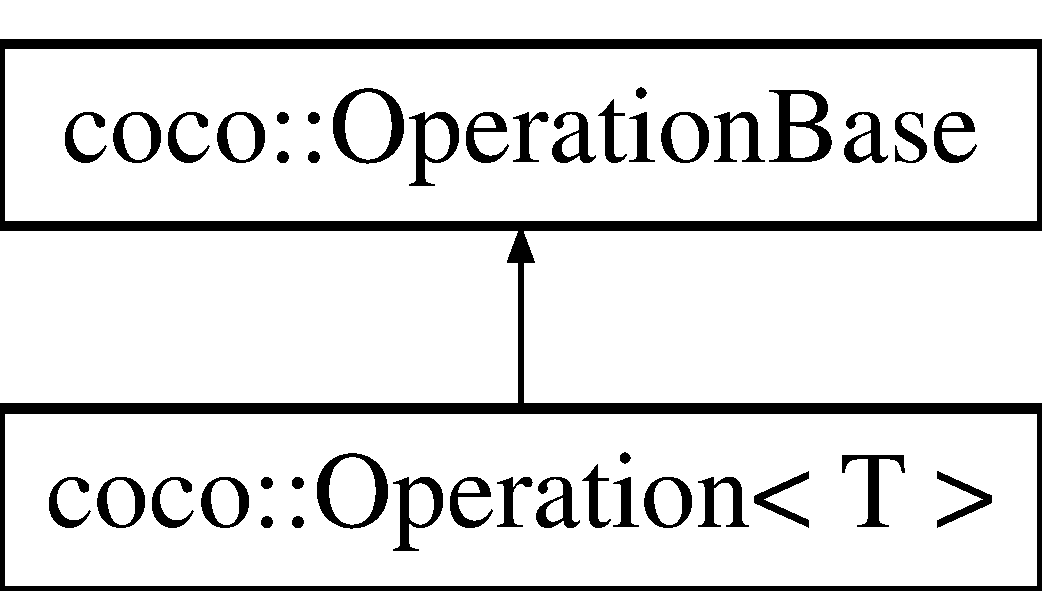
\includegraphics[height=2.000000cm]{classcoco_1_1_operation_base}
\end{center}
\end{figure}
\subsection*{Public Member Functions}
\begin{DoxyCompactItemize}
\item 
\hypertarget{classcoco_1_1_operation_base_aae9b74463779d30dca29a439213b7066}{}{\bfseries Operation\+Base} (\hyperlink{classcoco_1_1_service}{Service} $\ast$p, const std\+::string \&\hyperlink{classcoco_1_1_operation_base_aee0ff9e503d67abe3260e808fec4a183}{name})\label{classcoco_1_1_operation_base_aae9b74463779d30dca29a439213b7066}

\item 
virtual void $\ast$ \hyperlink{classcoco_1_1_operation_base_a298735d41b5fa6f69ecbcec833e4127f}{asfx} ()=0
\begin{DoxyCompactList}\small\item\em commented for future impl \end{DoxyCompactList}\item 
\hypertarget{classcoco_1_1_operation_base_a858f1db28251468bba10f25b858851d7}{}virtual const std\+::type\+\_\+info \& \hyperlink{classcoco_1_1_operation_base_a858f1db28251468bba10f25b858851d7}{assig} ()=0\label{classcoco_1_1_operation_base_a858f1db28251468bba10f25b858851d7}

\begin{DoxyCompactList}\small\item\em returns the type signature \end{DoxyCompactList}\item 
\hypertarget{classcoco_1_1_operation_base_a3c71b11a14371ef3a160b49ff8b16dc9}{}{\footnotesize template$<$class Sig $>$ }\\std\+::function$<$ Sig $>$ \& \hyperlink{classcoco_1_1_operation_base_a3c71b11a14371ef3a160b49ff8b16dc9}{as} ()\label{classcoco_1_1_operation_base_a3c71b11a14371ef3a160b49ff8b16dc9}

\begin{DoxyCompactList}\small\item\em returns the function as Signature if it matches, otherwise raises exception \end{DoxyCompactList}\item 
\hypertarget{classcoco_1_1_operation_base_afe4be0f5e168e05e614cec82619a0eda}{}const std\+::string \& \hyperlink{classcoco_1_1_operation_base_afe4be0f5e168e05e614cec82619a0eda}{doc} () const \label{classcoco_1_1_operation_base_afe4be0f5e168e05e614cec82619a0eda}

\begin{DoxyCompactList}\small\item\em associated documentation \end{DoxyCompactList}\item 
\hypertarget{classcoco_1_1_operation_base_a05b507563ee0e79666045019ae7561ee}{}void \hyperlink{classcoco_1_1_operation_base_a05b507563ee0e79666045019ae7561ee}{doc} (const std\+::string \&d)\label{classcoco_1_1_operation_base_a05b507563ee0e79666045019ae7561ee}

\begin{DoxyCompactList}\small\item\em stores doc \end{DoxyCompactList}\item 
\hypertarget{classcoco_1_1_operation_base_aee0ff9e503d67abe3260e808fec4a183}{}const std\+::string \& \hyperlink{classcoco_1_1_operation_base_aee0ff9e503d67abe3260e808fec4a183}{name} () const \label{classcoco_1_1_operation_base_aee0ff9e503d67abe3260e808fec4a183}

\begin{DoxyCompactList}\small\item\em return the name of the operation \end{DoxyCompactList}\item 
\hypertarget{classcoco_1_1_operation_base_ad7ffc8db29f1e37139bdc480617f86e8}{}void \hyperlink{classcoco_1_1_operation_base_ad7ffc8db29f1e37139bdc480617f86e8}{name} (const std\+::string \&d)\label{classcoco_1_1_operation_base_ad7ffc8db29f1e37139bdc480617f86e8}

\begin{DoxyCompactList}\small\item\em set the name of the operation \end{DoxyCompactList}\end{DoxyCompactItemize}
\subsection*{Private Attributes}
\begin{DoxyCompactItemize}
\item 
\hypertarget{classcoco_1_1_operation_base_a1b97fe250ddf789fe543bee58b837cf6}{}std\+::string {\bfseries name\+\_\+}\label{classcoco_1_1_operation_base_a1b97fe250ddf789fe543bee58b837cf6}

\item 
\hypertarget{classcoco_1_1_operation_base_a502298604b76a6736508ed4d58ab192d}{}std\+::string \hyperlink{classcoco_1_1_operation_base_a502298604b76a6736508ed4d58ab192d}{doc\+\_\+}\label{classcoco_1_1_operation_base_a502298604b76a6736508ed4d58ab192d}

\begin{DoxyCompactList}\small\item\em name of the operation \end{DoxyCompactList}\end{DoxyCompactItemize}


\subsection{Detailed Description}
Basic Class for Operations 

\subsection{Member Function Documentation}
\hypertarget{classcoco_1_1_operation_base_a298735d41b5fa6f69ecbcec833e4127f}{}\index{coco\+::\+Operation\+Base@{coco\+::\+Operation\+Base}!asfx@{asfx}}
\index{asfx@{asfx}!coco\+::\+Operation\+Base@{coco\+::\+Operation\+Base}}
\subsubsection[{asfx}]{\setlength{\rightskip}{0pt plus 5cm}virtual void$\ast$ coco\+::\+Operation\+Base\+::asfx (
\begin{DoxyParamCaption}
{}
\end{DoxyParamCaption}
)\hspace{0.3cm}{\ttfamily [pure virtual]}}\label{classcoco_1_1_operation_base_a298735d41b5fa6f69ecbcec833e4127f}


commented for future impl 

returns the contained function pointer 

Implemented in \hyperlink{classcoco_1_1_operation_a14160906142cffe52eaf2899dcd89c97}{coco\+::\+Operation$<$ T $>$}.



Referenced by as().



The documentation for this class was generated from the following files\+:\begin{DoxyCompactItemize}
\item 
src/coco\+\_\+core.\+hpp\item 
src/coco\+\_\+core.\+cpp\end{DoxyCompactItemize}

\hypertarget{classcoco_1_1_output_port}{}\section{coco\+:\+:Output\+Port$<$ T $>$ Class Template Reference}
\label{classcoco_1_1_output_port}\index{coco\+::\+Output\+Port$<$ T $>$@{coco\+::\+Output\+Port$<$ T $>$}}


Class representing an output port containing data of type T.  




{\ttfamily \#include $<$coco\+\_\+core.\+hpp$>$}

Inheritance diagram for coco\+:\+:Output\+Port$<$ T $>$\+:\begin{figure}[H]
\begin{center}
\leavevmode
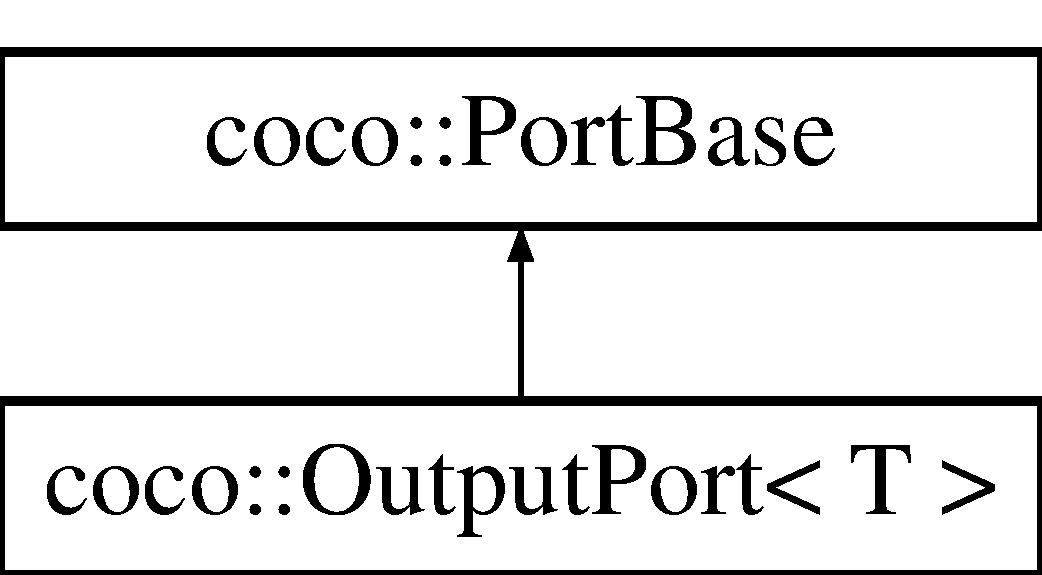
\includegraphics[height=2.000000cm]{classcoco_1_1_output_port}
\end{center}
\end{figure}
\subsection*{Public Member Functions}
\begin{DoxyCompactItemize}
\item 
\hypertarget{classcoco_1_1_output_port_a3f9c807795a223f1b5d74149e6b96b41}{}\hyperlink{classcoco_1_1_output_port_a3f9c807795a223f1b5d74149e6b96b41}{Output\+Port} (\hyperlink{classcoco_1_1_task_context}{Task\+Context} $\ast$p, const std\+::string \&\hyperlink{classcoco_1_1_port_base_abf4eb7fcc3ec9973ee73dd140e7646db}{name})\label{classcoco_1_1_output_port_a3f9c807795a223f1b5d74149e6b96b41}

\begin{DoxyCompactList}\small\item\em Simply call \hyperlink{classcoco_1_1_port_base}{Port\+Base} constructor. \end{DoxyCompactList}\item 
\hypertarget{classcoco_1_1_output_port_af98baef0b2f5e221b1023bfab6bbad57}{}const std\+::type\+\_\+info \& \hyperlink{classcoco_1_1_output_port_af98baef0b2f5e221b1023bfab6bbad57}{get\+Type\+Info} () const override\label{classcoco_1_1_output_port_af98baef0b2f5e221b1023bfab6bbad57}

\begin{DoxyCompactList}\small\item\em Get the type of the Port variable. \end{DoxyCompactList}\item 
\hypertarget{classcoco_1_1_output_port_a017669d64d3345abab16c2f046326147}{}bool \hyperlink{classcoco_1_1_output_port_a017669d64d3345abab16c2f046326147}{connect\+To} (\hyperlink{classcoco_1_1_port_base}{Port\+Base} $\ast$other, \hyperlink{structcoco_1_1_connection_policy}{Connection\+Policy} policy)\label{classcoco_1_1_output_port_a017669d64d3345abab16c2f046326147}

\begin{DoxyCompactList}\small\item\em Connect with an \hyperlink{classcoco_1_1_input_port}{Input\+Port}. \end{DoxyCompactList}\item 
\hypertarget{classcoco_1_1_output_port_a0605797751243903e6392b5814093e03}{}void \hyperlink{classcoco_1_1_output_port_a0605797751243903e6392b5814093e03}{write} (T \&input)\label{classcoco_1_1_output_port_a0605797751243903e6392b5814093e03}

\begin{DoxyCompactList}\small\item\em Writes in each of its connections {\ttfamily input}. \end{DoxyCompactList}\item 
\hypertarget{classcoco_1_1_output_port_a124e9820fb88d0497d99fdf0b3bd6f9c}{}void {\bfseries write} (T \&input, const std\+::string \&\hyperlink{classcoco_1_1_port_base_abf4eb7fcc3ec9973ee73dd140e7646db}{name})\label{classcoco_1_1_output_port_a124e9820fb88d0497d99fdf0b3bd6f9c}

\end{DoxyCompactItemize}
\subsection*{Private Member Functions}
\begin{DoxyCompactItemize}
\item 
\hypertarget{classcoco_1_1_output_port_a3cfb5103a317583146b7d3697ae78230}{}std\+::shared\+\_\+ptr$<$ \hyperlink{classcoco_1_1_connection_t}{Connection\+T}$<$ T $>$ $>$ \hyperlink{classcoco_1_1_output_port_a3cfb5103a317583146b7d3697ae78230}{get\+Connection} (int index)\label{classcoco_1_1_output_port_a3cfb5103a317583146b7d3697ae78230}

\begin{DoxyCompactList}\small\item\em Get the connection at position {\ttfamily index}. \end{DoxyCompactList}\item 
\hypertarget{classcoco_1_1_output_port_acc332d8226110146626fcbdf78d36713}{}std\+::shared\+\_\+ptr$<$ \hyperlink{classcoco_1_1_connection_t}{Connection\+T}$<$ T $>$ $>$ \hyperlink{classcoco_1_1_output_port_acc332d8226110146626fcbdf78d36713}{get\+Connection} (const std\+::string \&\hyperlink{classcoco_1_1_port_base_abf4eb7fcc3ec9973ee73dd140e7646db}{name})\label{classcoco_1_1_output_port_acc332d8226110146626fcbdf78d36713}

\begin{DoxyCompactList}\small\item\em Get the connection with component {\ttfamily name}. \end{DoxyCompactList}\item 
\hypertarget{classcoco_1_1_output_port_aee7aa5a4c469f686d560fd9b3ddb78e1}{}bool \hyperlink{classcoco_1_1_output_port_aee7aa5a4c469f686d560fd9b3ddb78e1}{connect\+To\+Typed} (\hyperlink{classcoco_1_1_input_port}{Input\+Port}$<$ T $>$ $\ast$other, \hyperlink{structcoco_1_1_connection_policy}{Connection\+Policy} policy)\label{classcoco_1_1_output_port_aee7aa5a4c469f686d560fd9b3ddb78e1}

\begin{DoxyCompactList}\small\item\em Connect the current port with {\ttfamily other}. \end{DoxyCompactList}\end{DoxyCompactItemize}
\subsection*{Additional Inherited Members}


\subsection{Detailed Description}
\subsubsection*{template$<$class T$>$class coco\+::\+Output\+Port$<$ T $>$}

Class representing an output port containing data of type T. 

The documentation for this class was generated from the following file\+:\begin{DoxyCompactItemize}
\item 
src/coco\+\_\+core.\+hpp\end{DoxyCompactItemize}

\hypertarget{classcoco_1_1_parallel_activity}{\section{coco\-:\-:Parallel\-Activity Class Reference}
\label{classcoco_1_1_parallel_activity}\index{coco\-::\-Parallel\-Activity@{coco\-::\-Parallel\-Activity}}
}


{\ttfamily \#include $<$ezoro.\-hpp$>$}

Inheritance diagram for coco\-:\-:Parallel\-Activity\-:\begin{figure}[H]
\begin{center}
\leavevmode
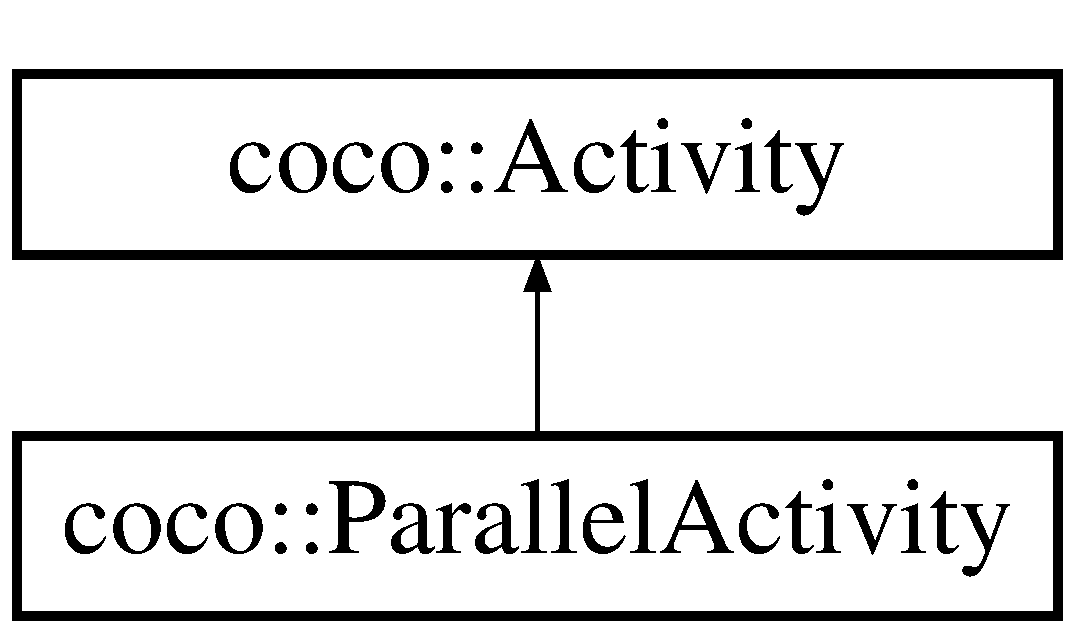
\includegraphics[height=2.000000cm]{classcoco_1_1_parallel_activity}
\end{center}
\end{figure}
\subsection*{Public Member Functions}
\begin{DoxyCompactItemize}
\item 
\hypertarget{classcoco_1_1_parallel_activity_ab3446f590315a0d5ba42fb84bff6641f}{\hyperlink{classcoco_1_1_parallel_activity_ab3446f590315a0d5ba42fb84bff6641f}{Parallel\-Activity} (\hyperlink{structcoco_1_1_schedule_policy}{Schedule\-Policy} policy, std\-::shared\-\_\-ptr$<$ \hyperlink{classcoco_1_1_runnable_interface}{Runnable\-Interface} $>$ r=nullptr)}\label{classcoco_1_1_parallel_activity_ab3446f590315a0d5ba42fb84bff6641f}

\begin{DoxyCompactList}\small\item\em simply call \hyperlink{classcoco_1_1_activity}{Activity} constructor \end{DoxyCompactList}\item 
\hypertarget{classcoco_1_1_parallel_activity_aa642be0f3fd844cfced97cabadd59dfe}{virtual void \hyperlink{classcoco_1_1_parallel_activity_aa642be0f3fd844cfced97cabadd59dfe}{start} () override}\label{classcoco_1_1_parallel_activity_aa642be0f3fd844cfced97cabadd59dfe}

\begin{DoxyCompactList}\small\item\em Start the activity. \end{DoxyCompactList}\item 
\hypertarget{classcoco_1_1_parallel_activity_a32e121790e325add143e5f9411ac75a4}{virtual void \hyperlink{classcoco_1_1_parallel_activity_a32e121790e325add143e5f9411ac75a4}{stop} () override}\label{classcoco_1_1_parallel_activity_a32e121790e325add143e5f9411ac75a4}

\begin{DoxyCompactList}\small\item\em Stop the activity. \end{DoxyCompactList}\item 
\hypertarget{classcoco_1_1_parallel_activity_a6d5004facadbbae85c5e98979dc1e301}{virtual void \hyperlink{classcoco_1_1_parallel_activity_a6d5004facadbbae85c5e98979dc1e301}{trigger} () override}\label{classcoco_1_1_parallel_activity_a6d5004facadbbae85c5e98979dc1e301}

\begin{DoxyCompactList}\small\item\em in case of a T\-R\-I\-G\-G\-E\-R activity starts one step of the execution \end{DoxyCompactList}\end{DoxyCompactItemize}
\subsection*{Protected Member Functions}
\begin{DoxyCompactItemize}
\item 
\hypertarget{classcoco_1_1_parallel_activity_a320a783acbe011c53fed23747336e713}{void \hyperlink{classcoco_1_1_parallel_activity_a320a783acbe011c53fed23747336e713}{entry} () override}\label{classcoco_1_1_parallel_activity_a320a783acbe011c53fed23747336e713}

\begin{DoxyCompactList}\small\item\em main execution function \end{DoxyCompactList}\end{DoxyCompactItemize}
\subsection*{Protected Attributes}
\begin{DoxyCompactItemize}
\item 
\hypertarget{classcoco_1_1_parallel_activity_ae874a1d7b5a96573d823f559fb536952}{std\-::unique\-\_\-ptr$<$ std\-::thread $>$ {\bfseries thread\-\_\-}}\label{classcoco_1_1_parallel_activity_ae874a1d7b5a96573d823f559fb536952}

\item 
\hypertarget{classcoco_1_1_parallel_activity_a287ffe32ef172b36bf2d409aace9d521}{std\-::mutex {\bfseries mutex\-\_\-t\-\_\-}}\label{classcoco_1_1_parallel_activity_a287ffe32ef172b36bf2d409aace9d521}

\item 
\hypertarget{classcoco_1_1_parallel_activity_a1dcd65a0e7e115c3deebdebd2e8646a1}{std\-::condition\-\_\-variable {\bfseries cond\-\_\-}}\label{classcoco_1_1_parallel_activity_a1dcd65a0e7e115c3deebdebd2e8646a1}

\end{DoxyCompactItemize}


\subsection{Detailed Description}
Uses thread 

The documentation for this class was generated from the following files\-:\begin{DoxyCompactItemize}
\item 
src/ezoro.\-hpp\item 
src/ezoro.\-cpp\end{DoxyCompactItemize}

\input{classcoco_1_1_peer_task}
\input{classcoco_1_1_peer_task_t}
\hypertarget{structstd_1_1placeholder__template}{\section{std\-:\-:placeholder\-\_\-template$<$ int $>$ Struct Template Reference}
\label{structstd_1_1placeholder__template}\index{std\-::placeholder\-\_\-template$<$ int $>$@{std\-::placeholder\-\_\-template$<$ int $>$}}
}


The documentation for this struct was generated from the following file\-:\begin{DoxyCompactItemize}
\item 
src/ezoro.\-hpp\end{DoxyCompactItemize}

\input{classcoco_1_1_pooled_channel}
\hypertarget{classcoco_1_1_port_base}{}\section{coco\+:\+:Port\+Base Class Reference}
\label{classcoco_1_1_port_base}\index{coco\+::\+Port\+Base@{coco\+::\+Port\+Base}}


Base class to manage ports.  




{\ttfamily \#include $<$coco\+\_\+core.\+hpp$>$}

Inheritance diagram for coco\+:\+:Port\+Base\+:\begin{figure}[H]
\begin{center}
\leavevmode
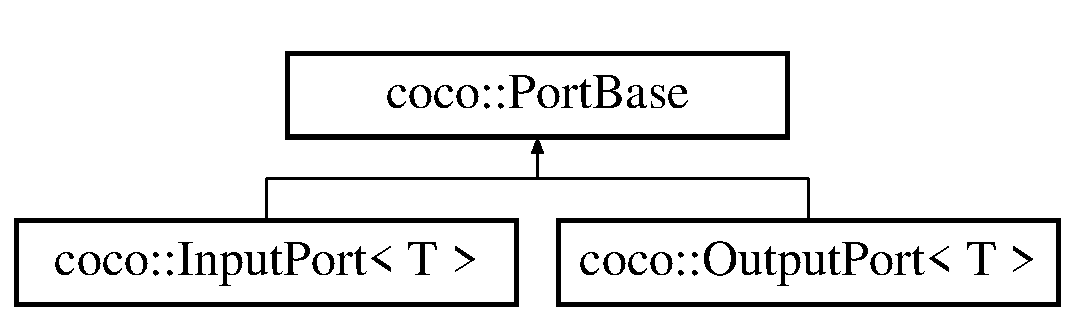
\includegraphics[height=2.000000cm]{classcoco_1_1_port_base}
\end{center}
\end{figure}
\subsection*{Public Member Functions}
\begin{DoxyCompactItemize}
\item 
\hypertarget{classcoco_1_1_port_base_a57e506ec75f7e6760fcf2cdfa8450d99}{}\hyperlink{classcoco_1_1_port_base_a57e506ec75f7e6760fcf2cdfa8450d99}{Port\+Base} (\hyperlink{classcoco_1_1_task_context}{Task\+Context} $\ast$p, const std\+::string \&\hyperlink{classcoco_1_1_port_base_abf4eb7fcc3ec9973ee73dd140e7646db}{name}, bool is\+\_\+output, bool is\+\_\+event)\label{classcoco_1_1_port_base_a57e506ec75f7e6760fcf2cdfa8450d99}

\begin{DoxyCompactList}\small\item\em Initialize input and output ports. \end{DoxyCompactList}\item 
\hypertarget{classcoco_1_1_port_base_af8a455d7672cb6f13aa37cee2a9acc94}{}virtual const std\+::type\+\_\+info \& \hyperlink{classcoco_1_1_port_base_af8a455d7672cb6f13aa37cee2a9acc94}{get\+Type\+Info} () const =0\label{classcoco_1_1_port_base_af8a455d7672cb6f13aa37cee2a9acc94}

\begin{DoxyCompactList}\small\item\em Return the template type name of the port data. \end{DoxyCompactList}\item 
\hypertarget{classcoco_1_1_port_base_abc0fcdf9a73f1f8e66905feb2dc2b374}{}virtual bool \hyperlink{classcoco_1_1_port_base_abc0fcdf9a73f1f8e66905feb2dc2b374}{connect\+To} (\hyperlink{classcoco_1_1_port_base}{Port\+Base} $\ast$, \hyperlink{structcoco_1_1_connection_policy}{Connection\+Policy} policy)=0\label{classcoco_1_1_port_base_abc0fcdf9a73f1f8e66905feb2dc2b374}

\begin{DoxyCompactList}\small\item\em Connect a port to another with a specified \hyperlink{structcoco_1_1_connection_policy}{Connection\+Policy}. \end{DoxyCompactList}\item 
\hypertarget{classcoco_1_1_port_base_aca58d449d57e44cb7d47cdeb543e8b8f}{}bool \hyperlink{classcoco_1_1_port_base_aca58d449d57e44cb7d47cdeb543e8b8f}{is\+Connected} () const \label{classcoco_1_1_port_base_aca58d449d57e44cb7d47cdeb543e8b8f}

\begin{DoxyCompactList}\small\item\em Return true if this port is connected to another one. \end{DoxyCompactList}\item 
\hypertarget{classcoco_1_1_port_base_a161986c4e70cdbc6df2664aafb197e0c}{}bool \hyperlink{classcoco_1_1_port_base_a161986c4e70cdbc6df2664aafb197e0c}{is\+Event} () const \label{classcoco_1_1_port_base_a161986c4e70cdbc6df2664aafb197e0c}

\begin{DoxyCompactList}\small\item\em Return true if this port is of type event. \end{DoxyCompactList}\item 
\hypertarget{classcoco_1_1_port_base_a8aed63e197daab4129a50dee5bf728fc}{}bool \hyperlink{classcoco_1_1_port_base_a8aed63e197daab4129a50dee5bf728fc}{is\+Output} () const \label{classcoco_1_1_port_base_a8aed63e197daab4129a50dee5bf728fc}

\begin{DoxyCompactList}\small\item\em Return true if this port is an output port. \end{DoxyCompactList}\item 
\hypertarget{classcoco_1_1_port_base_a8de69f58ac8d4110b51cba2616dc0ebc}{}void \hyperlink{classcoco_1_1_port_base_a8de69f58ac8d4110b51cba2616dc0ebc}{trigger\+Component} ()\label{classcoco_1_1_port_base_a8de69f58ac8d4110b51cba2616dc0ebc}

\begin{DoxyCompactList}\small\item\em Trigger the task to notify new dara is present in the port. \end{DoxyCompactList}\item 
\hypertarget{classcoco_1_1_port_base_a71bb264f74c371d2f988de9b383c8a1e}{}const std\+::string \& \hyperlink{classcoco_1_1_port_base_a71bb264f74c371d2f988de9b383c8a1e}{doc} () const \label{classcoco_1_1_port_base_a71bb264f74c371d2f988de9b383c8a1e}

\begin{DoxyCompactList}\small\item\em associated documentation \end{DoxyCompactList}\item 
\hypertarget{classcoco_1_1_port_base_ae79cc93c196c650ddef9fd14f6ba5c80}{}void \hyperlink{classcoco_1_1_port_base_ae79cc93c196c650ddef9fd14f6ba5c80}{doc} (const std\+::string \&d)\label{classcoco_1_1_port_base_ae79cc93c196c650ddef9fd14f6ba5c80}

\begin{DoxyCompactList}\small\item\em stores doc \end{DoxyCompactList}\item 
\hypertarget{classcoco_1_1_port_base_abf4eb7fcc3ec9973ee73dd140e7646db}{}const std\+::string \& \hyperlink{classcoco_1_1_port_base_abf4eb7fcc3ec9973ee73dd140e7646db}{name} () const \label{classcoco_1_1_port_base_abf4eb7fcc3ec9973ee73dd140e7646db}

\begin{DoxyCompactList}\small\item\em Get the name of the port. \end{DoxyCompactList}\item 
\hypertarget{classcoco_1_1_port_base_a288503d386fa9cd3022fe4437b377e5b}{}void \hyperlink{classcoco_1_1_port_base_a288503d386fa9cd3022fe4437b377e5b}{name} (const std\+::string \&d)\label{classcoco_1_1_port_base_a288503d386fa9cd3022fe4437b377e5b}

\begin{DoxyCompactList}\small\item\em Set the name of the port. \end{DoxyCompactList}\item 
\hypertarget{classcoco_1_1_port_base_ab2ec3f4ef49a5afec734149b75644709}{}int \hyperlink{classcoco_1_1_port_base_ab2ec3f4ef49a5afec734149b75644709}{connections\+Count} () const \label{classcoco_1_1_port_base_ab2ec3f4ef49a5afec734149b75644709}

\begin{DoxyCompactList}\small\item\em Returns the number of connections associate to this port. \end{DoxyCompactList}\item 
\hypertarget{classcoco_1_1_port_base_afbcff166e210e06142a9bbfb9c8c03f3}{}std\+::string \hyperlink{classcoco_1_1_port_base_afbcff166e210e06142a9bbfb9c8c03f3}{task\+Name} () const \label{classcoco_1_1_port_base_afbcff166e210e06142a9bbfb9c8c03f3}

\begin{DoxyCompactList}\small\item\em Return the name of the task owing this connection. \end{DoxyCompactList}\end{DoxyCompactItemize}
\subsection*{Protected Member Functions}
\begin{DoxyCompactItemize}
\item 
\hypertarget{classcoco_1_1_port_base_afa50a47a0608471a7e182c5f848193ca}{}bool \hyperlink{classcoco_1_1_port_base_afa50a47a0608471a7e182c5f848193ca}{add\+Connection} (std\+::shared\+\_\+ptr$<$ \hyperlink{classcoco_1_1_connection_base}{Connection\+Base} $>$ connection)\label{classcoco_1_1_port_base_afa50a47a0608471a7e182c5f848193ca}

\begin{DoxyCompactList}\small\item\em Add a connection to the \hyperlink{classcoco_1_1_connection_manager}{Connection\+Manager}. \end{DoxyCompactList}\end{DoxyCompactItemize}
\subsection*{Protected Attributes}
\begin{DoxyCompactItemize}
\item 
\hypertarget{classcoco_1_1_port_base_a33f04beb590390a25bfdcf300bffb70e}{}\hyperlink{classcoco_1_1_connection_manager}{Connection\+Manager} {\bfseries manager\+\_\+} = \{ this \}\label{classcoco_1_1_port_base_a33f04beb590390a25bfdcf300bffb70e}

\item 
\hypertarget{classcoco_1_1_port_base_af6fede884062c2b3a774ed69da5c0291}{}std\+::shared\+\_\+ptr$<$ \hyperlink{classcoco_1_1_task_context}{Task\+Context} $>$ {\bfseries task\+\_\+}\label{classcoco_1_1_port_base_af6fede884062c2b3a774ed69da5c0291}

\item 
\hypertarget{classcoco_1_1_port_base_a3ca4d9d5dcd73da483b176fdd45cb837}{}std\+::string \hyperlink{classcoco_1_1_port_base_a3ca4d9d5dcd73da483b176fdd45cb837}{name\+\_\+}\label{classcoco_1_1_port_base_a3ca4d9d5dcd73da483b176fdd45cb837}

\begin{DoxyCompactList}\small\item\em Task using this port. \end{DoxyCompactList}\item 
\hypertarget{classcoco_1_1_port_base_ab821e90d50ec2c6f8c1edde95272719c}{}std\+::string {\bfseries doc\+\_\+}\label{classcoco_1_1_port_base_ab821e90d50ec2c6f8c1edde95272719c}

\item 
\hypertarget{classcoco_1_1_port_base_a3bda6ce2261f36704a7f30dfed297426}{}bool {\bfseries is\+\_\+event\+\_\+}\label{classcoco_1_1_port_base_a3bda6ce2261f36704a7f30dfed297426}

\item 
\hypertarget{classcoco_1_1_port_base_a6119b0d7b6bb1eabf085afb7f3bc149f}{}bool {\bfseries is\+\_\+output\+\_\+}\label{classcoco_1_1_port_base_a6119b0d7b6bb1eabf085afb7f3bc149f}

\end{DoxyCompactItemize}
\subsection*{Friends}
\begin{DoxyCompactItemize}
\item 
\hypertarget{classcoco_1_1_port_base_aa750daec74c1bf813c092ea268f3b8f8}{}{\footnotesize template$<$class T $>$ }\\class {\bfseries Input\+Port}\label{classcoco_1_1_port_base_aa750daec74c1bf813c092ea268f3b8f8}

\item 
\hypertarget{classcoco_1_1_port_base_a1b667fb33da7060c4747eeafcd85db20}{}{\footnotesize template$<$class T $>$ }\\class {\bfseries Output\+Port}\label{classcoco_1_1_port_base_a1b667fb33da7060c4747eeafcd85db20}

\end{DoxyCompactItemize}


\subsection{Detailed Description}
Base class to manage ports. 

The documentation for this class was generated from the following files\+:\begin{DoxyCompactItemize}
\item 
src/coco\+\_\+core.\+hpp\item 
src/coco\+\_\+core.\+cpp\end{DoxyCompactItemize}

\input{classcoco_1_1_port_pooled}
\input{classcoco_1_1_profiler}
\input{classcoco_1_1_profiler_manager}
\hypertarget{classcoco_1_1_runnable_interface}{}\section{coco\+:\+:Runnable\+Interface Class Reference}
\label{classcoco_1_1_runnable_interface}\index{coco\+::\+Runnable\+Interface@{coco\+::\+Runnable\+Interface}}


Interface class to execute the components.  




{\ttfamily \#include $<$coco\+\_\+core.\+hpp$>$}

Inheritance diagram for coco\+:\+:Runnable\+Interface\+:\begin{figure}[H]
\begin{center}
\leavevmode
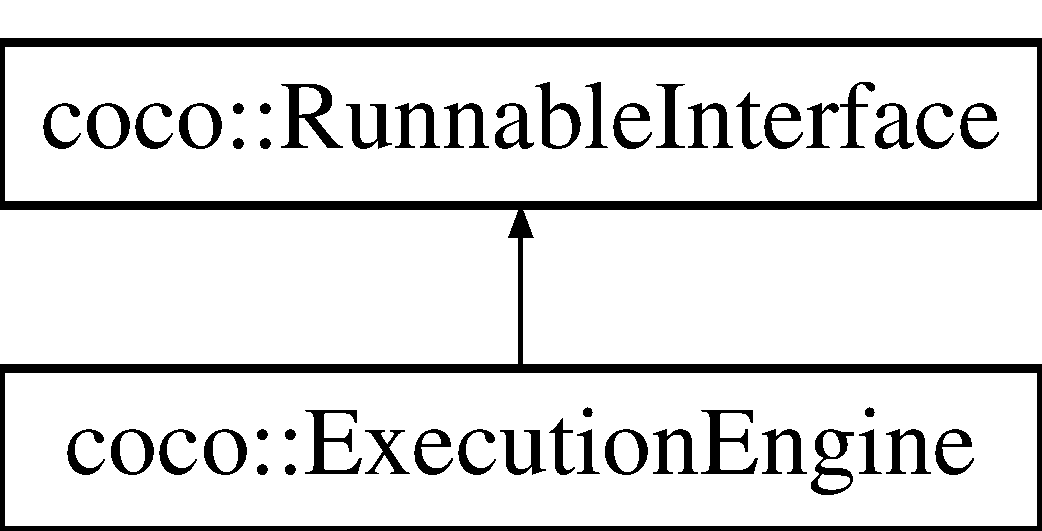
\includegraphics[height=2.000000cm]{classcoco_1_1_runnable_interface}
\end{center}
\end{figure}
\subsection*{Public Member Functions}
\begin{DoxyCompactItemize}
\item 
\hypertarget{classcoco_1_1_runnable_interface_aa104a540e574daa30a7b113150ccf0fb}{}virtual void \hyperlink{classcoco_1_1_runnable_interface_aa104a540e574daa30a7b113150ccf0fb}{init} ()=0\label{classcoco_1_1_runnable_interface_aa104a540e574daa30a7b113150ccf0fb}

\begin{DoxyCompactList}\small\item\em Initialize the components members. \end{DoxyCompactList}\item 
\hypertarget{classcoco_1_1_runnable_interface_a056e59ec3ee688ad7c35ebbf2c1a7d87}{}virtual void \hyperlink{classcoco_1_1_runnable_interface_a056e59ec3ee688ad7c35ebbf2c1a7d87}{step} ()=0\label{classcoco_1_1_runnable_interface_a056e59ec3ee688ad7c35ebbf2c1a7d87}

\begin{DoxyCompactList}\small\item\em If the task is running execute uno step of the execution function. \end{DoxyCompactList}\item 
\hypertarget{classcoco_1_1_runnable_interface_acbe1640138c6d48f23ba53c821663419}{}virtual void \hyperlink{classcoco_1_1_runnable_interface_acbe1640138c6d48f23ba53c821663419}{finalize} ()=0\label{classcoco_1_1_runnable_interface_acbe1640138c6d48f23ba53c821663419}

\begin{DoxyCompactList}\small\item\em When the task is stopped clear all the members. \end{DoxyCompactList}\end{DoxyCompactItemize}


\subsection{Detailed Description}
Interface class to execute the components. 

The documentation for this class was generated from the following file\+:\begin{DoxyCompactItemize}
\item 
src/coco\+\_\+core.\+hpp\end{DoxyCompactItemize}

\hypertarget{structcoco_1_1_schedule_policy}{\section{coco\-:\-:Schedule\-Policy Struct Reference}
\label{structcoco_1_1_schedule_policy}\index{coco\-::\-Schedule\-Policy@{coco\-::\-Schedule\-Policy}}
}


policy for executing the component  




{\ttfamily \#include $<$ezoro.\-hpp$>$}

\subsection*{Public Types}
\begin{DoxyCompactItemize}
\item 
enum {\bfseries Policy} \{ {\bfseries P\-E\-R\-I\-O\-D\-I\-C}, 
{\bfseries H\-A\-R\-D}, 
{\bfseries T\-R\-I\-G\-G\-E\-R\-E\-D}
 \}
\end{DoxyCompactItemize}
\subsection*{Public Member Functions}
\begin{DoxyCompactItemize}
\item 
\hypertarget{structcoco_1_1_schedule_policy_a10ca5e9aacf647c410a160cf6981ba1b}{{\bfseries Schedule\-Policy} (Policy policy=P\-E\-R\-I\-O\-D\-I\-C, int period=1)}\label{structcoco_1_1_schedule_policy_a10ca5e9aacf647c410a160cf6981ba1b}

\end{DoxyCompactItemize}
\subsection*{Public Attributes}
\begin{DoxyCompactItemize}
\item 
\hypertarget{structcoco_1_1_schedule_policy_ab1d0eb6297cf9b1630d56b24ca56e0ce}{Policy {\bfseries timing\-\_\-policy\-\_\-} = P\-E\-R\-I\-O\-D\-I\-C}\label{structcoco_1_1_schedule_policy_ab1d0eb6297cf9b1630d56b24ca56e0ce}

\item 
\hypertarget{structcoco_1_1_schedule_policy_a1c4cad7562e9b30fdae43e8be3708b6e}{int {\bfseries period\-\_\-ms\-\_\-}}\label{structcoco_1_1_schedule_policy_a1c4cad7562e9b30fdae43e8be3708b6e}

\item 
\hypertarget{structcoco_1_1_schedule_policy_ac2019bc1c226a87b984d6e4a40a3219f}{std\-::string {\bfseries trigger\-\_\-}}\label{structcoco_1_1_schedule_policy_ac2019bc1c226a87b984d6e4a40a3219f}

\end{DoxyCompactItemize}


\subsection{Detailed Description}
policy for executing the component 

The documentation for this struct was generated from the following file\-:\begin{DoxyCompactItemize}
\item 
src/ezoro.\-hpp\end{DoxyCompactItemize}

\input{structcoco_1_1scopedxml}
\hypertarget{classcoco_1_1_sequential_activity}{\section{coco\-:\-:Sequential\-Activity Class Reference}
\label{classcoco_1_1_sequential_activity}\index{coco\-::\-Sequential\-Activity@{coco\-::\-Sequential\-Activity}}
}


{\ttfamily \#include $<$ezoro.\-hpp$>$}

Inheritance diagram for coco\-:\-:Sequential\-Activity\-:\begin{figure}[H]
\begin{center}
\leavevmode
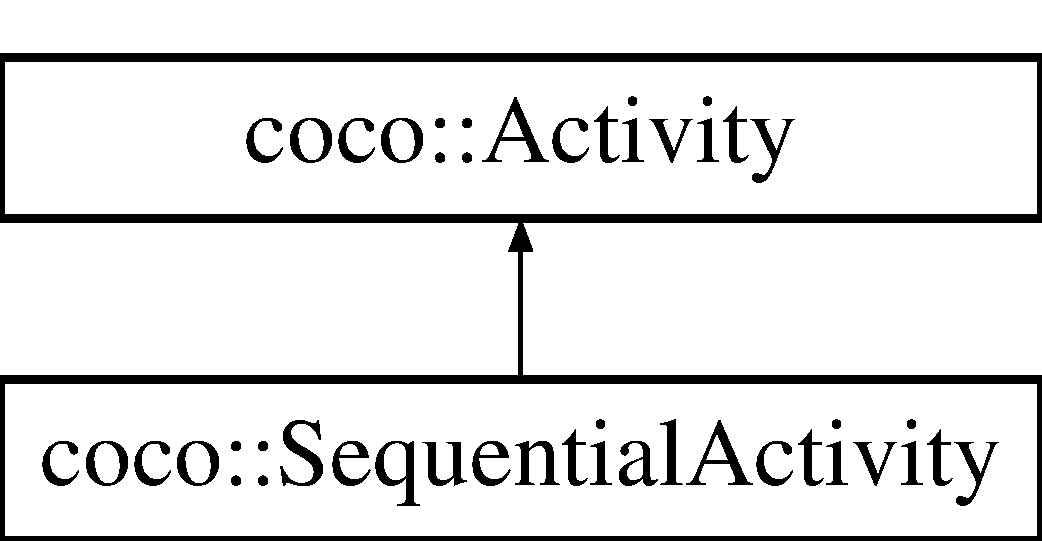
\includegraphics[height=2.000000cm]{classcoco_1_1_sequential_activity}
\end{center}
\end{figure}
\subsection*{Public Member Functions}
\begin{DoxyCompactItemize}
\item 
\hypertarget{classcoco_1_1_sequential_activity_ac7ba1d0816d9ab6cbf43493e64e48ecd}{{\bfseries Sequential\-Activity} (\hyperlink{structcoco_1_1_schedule_policy}{Schedule\-Policy} policy, std\-::shared\-\_\-ptr$<$ \hyperlink{classcoco_1_1_runnable_interface}{Runnable\-Interface} $>$ r=nullptr)}\label{classcoco_1_1_sequential_activity_ac7ba1d0816d9ab6cbf43493e64e48ecd}

\item 
\hypertarget{classcoco_1_1_sequential_activity_a29995fe18e3162f0c04787d7db9bda19}{virtual void \hyperlink{classcoco_1_1_sequential_activity_a29995fe18e3162f0c04787d7db9bda19}{start} () override}\label{classcoco_1_1_sequential_activity_a29995fe18e3162f0c04787d7db9bda19}

\begin{DoxyCompactList}\small\item\em Start the activity. \end{DoxyCompactList}\item 
\hypertarget{classcoco_1_1_sequential_activity_ab1d6827509bee10cd26bbfae3b5fb857}{virtual void \hyperlink{classcoco_1_1_sequential_activity_ab1d6827509bee10cd26bbfae3b5fb857}{stop} () override}\label{classcoco_1_1_sequential_activity_ab1d6827509bee10cd26bbfae3b5fb857}

\begin{DoxyCompactList}\small\item\em Stop the activity. \end{DoxyCompactList}\item 
\hypertarget{classcoco_1_1_sequential_activity_a9e619d6d2df7e843cbbfeacd99193446}{virtual void \hyperlink{classcoco_1_1_sequential_activity_a9e619d6d2df7e843cbbfeacd99193446}{trigger} () override}\label{classcoco_1_1_sequential_activity_a9e619d6d2df7e843cbbfeacd99193446}

\begin{DoxyCompactList}\small\item\em in case of a T\-R\-I\-G\-G\-E\-R activity starts one step of the execution \end{DoxyCompactList}\end{DoxyCompactItemize}
\subsection*{Protected Member Functions}
\begin{DoxyCompactItemize}
\item 
\hypertarget{classcoco_1_1_sequential_activity_ac64d096bd0a06344cca6803c9874094d}{void \hyperlink{classcoco_1_1_sequential_activity_ac64d096bd0a06344cca6803c9874094d}{entry} () override}\label{classcoco_1_1_sequential_activity_ac64d096bd0a06344cca6803c9874094d}

\begin{DoxyCompactList}\small\item\em main execution function \end{DoxyCompactList}\end{DoxyCompactItemize}
\subsection*{Additional Inherited Members}


\subsection{Detailed Description}
No thread but thread safe 

The documentation for this class was generated from the following files\-:\begin{DoxyCompactItemize}
\item 
src/ezoro.\-hpp\item 
src/ezoro.\-cpp\end{DoxyCompactItemize}

\hypertarget{classcoco_1_1_service}{}\section{coco\+:\+:Service Class Reference}
\label{classcoco_1_1_service}\index{coco\+::\+Service@{coco\+::\+Service}}


Manages all properties of a Task Context. Services is present because Task Context can have sub ones.  




{\ttfamily \#include $<$coco\+\_\+core.\+hpp$>$}

Inheritance diagram for coco\+:\+:Service\+:\begin{figure}[H]
\begin{center}
\leavevmode
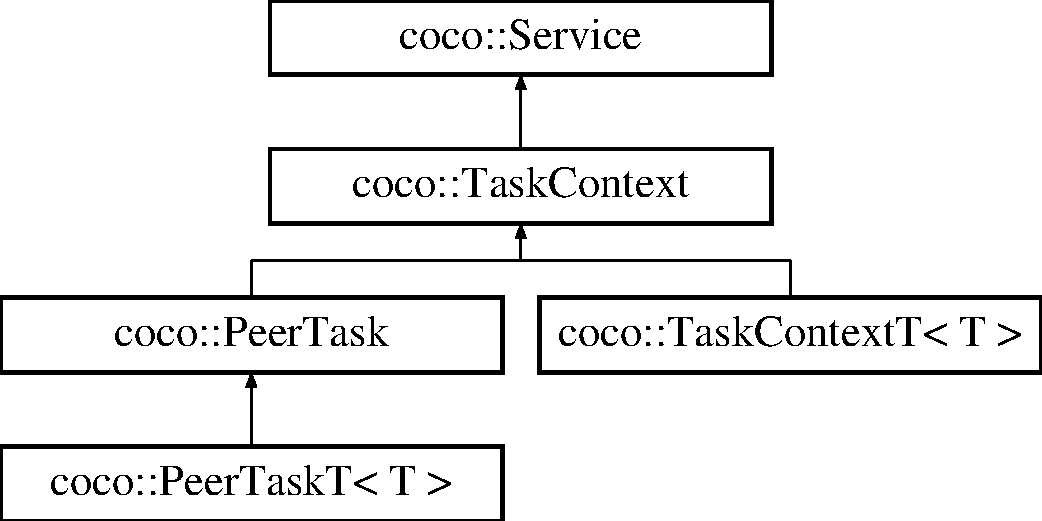
\includegraphics[height=4.000000cm]{classcoco_1_1_service}
\end{center}
\end{figure}
\subsection*{Public Member Functions}
\begin{DoxyCompactItemize}
\item 
\hypertarget{classcoco_1_1_service_afcdc2a94142f87cf2e86da7fc7973011}{}\hyperlink{classcoco_1_1_service_afcdc2a94142f87cf2e86da7fc7973011}{Service} (const std\+::string \&n=\char`\"{}\char`\"{})\label{classcoco_1_1_service_afcdc2a94142f87cf2e86da7fc7973011}

\begin{DoxyCompactList}\small\item\em Initialize \hyperlink{classcoco_1_1_service}{Service} name. \end{DoxyCompactList}\item 
\hypertarget{classcoco_1_1_service_abba97c5449141cf2b80caa818b815b0b}{}bool \hyperlink{classcoco_1_1_service_abba97c5449141cf2b80caa818b815b0b}{add\+Attribute} (\hyperlink{classcoco_1_1_attribute_base}{Attribute\+Base} $\ast$a)\label{classcoco_1_1_service_abba97c5449141cf2b80caa818b815b0b}

\begin{DoxyCompactList}\small\item\em Add an Atribute. \end{DoxyCompactList}\item 
\hypertarget{classcoco_1_1_service_a69fa3e93fbe6942d48e2736d401e3d8c}{}\hyperlink{classcoco_1_1_attribute_base}{Attribute\+Base} $\ast$ \hyperlink{classcoco_1_1_service_a69fa3e93fbe6942d48e2736d401e3d8c}{get\+Attribute} (std\+::string name)\label{classcoco_1_1_service_a69fa3e93fbe6942d48e2736d401e3d8c}

\begin{DoxyCompactList}\small\item\em Return an \hyperlink{classcoco_1_1_attribute_base}{Attribute\+Base} ptr. \end{DoxyCompactList}\item 
\hypertarget{classcoco_1_1_service_a5a557418f6e2b7767d8a9f39d80f8a97}{}{\footnotesize template$<$class T $>$ }\\T \& \hyperlink{classcoco_1_1_service_a5a557418f6e2b7767d8a9f39d80f8a97}{get\+Attribute\+Ref} (std\+::string name)\label{classcoco_1_1_service_a5a557418f6e2b7767d8a9f39d80f8a97}

\begin{DoxyCompactList}\small\item\em Return a reference to the variable managed by this attribute. \end{DoxyCompactList}\item 
\hypertarget{classcoco_1_1_service_a15c53f198c44b03b89ae78f38aaa00a9}{}\hyperlink{structcoco_1_1impl_1_1map__keys}{coco\+::impl\+::map\+\_\+keys}$<$ std\+::string, \hyperlink{classcoco_1_1_attribute_base}{Attribute\+Base} $\ast$ $>$ \hyperlink{classcoco_1_1_service_a15c53f198c44b03b89ae78f38aaa00a9}{get\+Attribute\+Names} ()\label{classcoco_1_1_service_a15c53f198c44b03b89ae78f38aaa00a9}

\begin{DoxyCompactList}\small\item\em Return a custo map to iterate over the keys. \end{DoxyCompactList}\item 
\hypertarget{classcoco_1_1_service_ac7ef2f278ddf72fab9e8dd1d2c03f277}{}\hyperlink{structcoco_1_1impl_1_1map__values}{coco\+::impl\+::map\+\_\+values}$<$ std\+::string, \hyperlink{classcoco_1_1_attribute_base}{Attribute\+Base} $\ast$ $>$ \hyperlink{classcoco_1_1_service_ac7ef2f278ddf72fab9e8dd1d2c03f277}{get\+Attributes} ()\label{classcoco_1_1_service_ac7ef2f278ddf72fab9e8dd1d2c03f277}

\begin{DoxyCompactList}\small\item\em Return a custo map to iterate over the values. \end{DoxyCompactList}\item 
\hypertarget{classcoco_1_1_service_a57fce01d8c5fc7b77058238a072d4fce}{}bool \hyperlink{classcoco_1_1_service_a57fce01d8c5fc7b77058238a072d4fce}{add\+Port} (\hyperlink{classcoco_1_1_port_base}{Port\+Base} $\ast$p)\label{classcoco_1_1_service_a57fce01d8c5fc7b77058238a072d4fce}

\begin{DoxyCompactList}\small\item\em Add a port to its list. \end{DoxyCompactList}\item 
\hypertarget{classcoco_1_1_service_a12e05c075e9fd899e795a1e929333c71}{}\hyperlink{classcoco_1_1_port_base}{Port\+Base} $\ast$ \hyperlink{classcoco_1_1_service_a12e05c075e9fd899e795a1e929333c71}{get\+Port} (std\+::string name)\label{classcoco_1_1_service_a12e05c075e9fd899e795a1e929333c71}

\begin{DoxyCompactList}\small\item\em Return a port based on its name. \end{DoxyCompactList}\item 
\hypertarget{classcoco_1_1_service_a5c2bcd05477b3058ac40de1d1c60e0c3}{}\hyperlink{structcoco_1_1impl_1_1map__keys}{coco\+::impl\+::map\+\_\+keys}$<$ std\+::string, \hyperlink{classcoco_1_1_port_base}{Port\+Base} $\ast$ $>$ {\bfseries get\+Port\+Names} ()\label{classcoco_1_1_service_a5c2bcd05477b3058ac40de1d1c60e0c3}

\item 
\hypertarget{classcoco_1_1_service_a9a980751ec51e1149302049d111d897f}{}\hyperlink{structcoco_1_1impl_1_1map__values}{coco\+::impl\+::map\+\_\+values}$<$ std\+::string, \hyperlink{classcoco_1_1_port_base}{Port\+Base} $\ast$ $>$ {\bfseries get\+Ports} ()\label{classcoco_1_1_service_a9a980751ec51e1149302049d111d897f}

\item 
\hypertarget{classcoco_1_1_service_ae0781be1829827b69d055fa89c8625c6}{}bool \hyperlink{classcoco_1_1_service_ae0781be1829827b69d055fa89c8625c6}{add\+Operation} (\hyperlink{classcoco_1_1_operation_base}{Operation\+Base} $\ast$o)\label{classcoco_1_1_service_ae0781be1829827b69d055fa89c8625c6}

\begin{DoxyCompactList}\small\item\em Add an operation from an existing ptr. \end{DoxyCompactList}\item 
\hypertarget{classcoco_1_1_service_a3ce8fa79ff5c68593d6a8229a95d396d}{}{\footnotesize template$<$class Function , class Obj $>$ }\\bool \hyperlink{classcoco_1_1_service_a3ce8fa79ff5c68593d6a8229a95d396d}{add\+Operation} (const std\+::string \&name, Function a, Obj b)\label{classcoco_1_1_service_a3ce8fa79ff5c68593d6a8229a95d396d}

\begin{DoxyCompactList}\small\item\em Create and add a new operation. \end{DoxyCompactList}\item 
\hypertarget{classcoco_1_1_service_a22606de3c858aae68d100c253cfc6c49}{}{\footnotesize template$<$class Function $>$ }\\bool \hyperlink{classcoco_1_1_service_a22606de3c858aae68d100c253cfc6c49}{add\+Operation} (const std\+::string \&name, Function f)\label{classcoco_1_1_service_a22606de3c858aae68d100c253cfc6c49}

\begin{DoxyCompactList}\small\item\em Create and add a new operation. \end{DoxyCompactList}\item 
\hypertarget{classcoco_1_1_service_a2649fc0bfef1e23b57d29bdf0a15e2d9}{}{\footnotesize template$<$class Sig $>$ }\\std\+::function$<$ Sig $>$ {\bfseries get\+Operation} (const std\+::string \&name)\label{classcoco_1_1_service_a2649fc0bfef1e23b57d29bdf0a15e2d9}

\item 
\hypertarget{classcoco_1_1_service_af6a8a7bfb1d4330ad0c3f22aa592a7d8}{}\hyperlink{structcoco_1_1impl_1_1map__keys}{coco\+::impl\+::map\+\_\+keys}$<$ std\+::string, \hyperlink{classcoco_1_1_operation_base}{Operation\+Base} $\ast$ $>$ {\bfseries get\+Operation\+Names} ()\label{classcoco_1_1_service_af6a8a7bfb1d4330ad0c3f22aa592a7d8}

\item 
\hypertarget{classcoco_1_1_service_aa61573f9c66d645e6d64fa839a2ea1ca}{}\hyperlink{structcoco_1_1impl_1_1map__values}{coco\+::impl\+::map\+\_\+values}$<$ std\+::string, \hyperlink{classcoco_1_1_operation_base}{Operation\+Base} $\ast$ $>$ {\bfseries get\+Operations} ()\label{classcoco_1_1_service_aa61573f9c66d645e6d64fa839a2ea1ca}

\item 
\hypertarget{classcoco_1_1_service_a1615d5bae6a780044894056ae085b6a0}{}bool {\bfseries has\+Pending} () const \label{classcoco_1_1_service_a1615d5bae6a780044894056ae085b6a0}

\item 
\hypertarget{classcoco_1_1_service_a4f7e3408bf16da826159d02cf610a609}{}void {\bfseries step\+Pending} ()\label{classcoco_1_1_service_a4f7e3408bf16da826159d02cf610a609}

\item 
\hypertarget{classcoco_1_1_service_a2dec5e9cc69971620700035e66cff74d}{}{\footnotesize template$<$class Sig , class... Args$>$ }\\bool {\bfseries enqueue\+Operation} (const std\+::string \&name, Args...\+args)\label{classcoco_1_1_service_a2dec5e9cc69971620700035e66cff74d}

\item 
\hypertarget{classcoco_1_1_service_a452f324bff06c6d9f13a9c04b0184a13}{}bool \hyperlink{classcoco_1_1_service_a452f324bff06c6d9f13a9c04b0184a13}{add\+Peer} (\hyperlink{classcoco_1_1_task_context}{Task\+Context} $\ast$p)\label{classcoco_1_1_service_a452f324bff06c6d9f13a9c04b0184a13}

\begin{DoxyCompactList}\small\item\em Add a peer. \end{DoxyCompactList}\item 
\hypertarget{classcoco_1_1_service_aa02f55a16b0446ea2a3c3e7fa163da2e}{}std\+::list$<$ \hyperlink{classcoco_1_1_task_context}{Task\+Context} $\ast$ $>$ {\bfseries get\+Peers} ()\label{classcoco_1_1_service_aa02f55a16b0446ea2a3c3e7fa163da2e}

\item 
\hypertarget{classcoco_1_1_service_ad5de0a202461a0bbbfcd4922f000574b}{}\hyperlink{structcoco_1_1impl_1_1map__keys}{coco\+::impl\+::map\+\_\+keys}$<$ std\+::string, std\+::unique\+\_\+ptr$<$ \hyperlink{classcoco_1_1_service}{Service} $>$ $>$ {\bfseries get\+Service\+Names} ()\label{classcoco_1_1_service_ad5de0a202461a0bbbfcd4922f000574b}

\item 
\hypertarget{classcoco_1_1_service_a5dbd858b1bbf99d641b6b63bc208a8e7}{}\hyperlink{structcoco_1_1impl_1_1map__values}{coco\+::impl\+::map\+\_\+values}$<$ std\+::string, std\+::unique\+\_\+ptr$<$ \hyperlink{classcoco_1_1_service}{Service} $>$ $>$ {\bfseries get\+Services} ()\label{classcoco_1_1_service_a5dbd858b1bbf99d641b6b63bc208a8e7}

\item 
\hypertarget{classcoco_1_1_service_ad73c4cdd616d7308174c9b40bf69489c}{}\hyperlink{classcoco_1_1_service}{Service} $\ast$ \hyperlink{classcoco_1_1_service_ad73c4cdd616d7308174c9b40bf69489c}{provides} ()\label{classcoco_1_1_service_ad73c4cdd616d7308174c9b40bf69489c}

\begin{DoxyCompactList}\small\item\em returns self as provider \end{DoxyCompactList}\item 
\hypertarget{classcoco_1_1_service_ae34998ed39c71b711e9d1939472a85b1}{}\hyperlink{classcoco_1_1_service}{Service} $\ast$ \hyperlink{classcoco_1_1_service_ae34998ed39c71b711e9d1939472a85b1}{provides} (const std\+::string \&x)\label{classcoco_1_1_service_ae34998ed39c71b711e9d1939472a85b1}

\begin{DoxyCompactList}\small\item\em check for sub services \end{DoxyCompactList}\item 
\hypertarget{classcoco_1_1_service_a71e9b86365eb33d81ef7dad93e4c37da}{}void {\bfseries set\+Name} (std\+::string name)\label{classcoco_1_1_service_a71e9b86365eb33d81ef7dad93e4c37da}

\item 
\hypertarget{classcoco_1_1_service_a36b9922e26da16acc55cc239b29fb02a}{}const std\+::string \& {\bfseries name} () const \label{classcoco_1_1_service_a36b9922e26da16acc55cc239b29fb02a}

\item 
\hypertarget{classcoco_1_1_service_ab95d453640ed30f7dd6741a0d56e7495}{}void {\bfseries set\+Instantiation\+Name} (const std\+::string \&name)\label{classcoco_1_1_service_ab95d453640ed30f7dd6741a0d56e7495}

\item 
\hypertarget{classcoco_1_1_service_a2b420c54cd8f4673d5e9c9561ab8d945}{}const std\+::string \& {\bfseries instantiation\+Name} () const \label{classcoco_1_1_service_a2b420c54cd8f4673d5e9c9561ab8d945}

\item 
\hypertarget{classcoco_1_1_service_a6d2d09b40b6b37dcf0b234c11ec8147d}{}void {\bfseries doc} (std\+::string xdoc)\label{classcoco_1_1_service_a6d2d09b40b6b37dcf0b234c11ec8147d}

\item 
\hypertarget{classcoco_1_1_service_ab0c36a1d9bba3bb88cd9b7899e7db920}{}const std\+::string \& {\bfseries doc} () const \label{classcoco_1_1_service_ab0c36a1d9bba3bb88cd9b7899e7db920}

\end{DoxyCompactItemize}
\subsection*{Private Attributes}
\begin{DoxyCompactItemize}
\item 
\hypertarget{classcoco_1_1_service_ab7810b45fabd24c1283e094b8cddb0a9}{}std\+::string {\bfseries name\+\_\+}\label{classcoco_1_1_service_ab7810b45fabd24c1283e094b8cddb0a9}

\item 
\hypertarget{classcoco_1_1_service_a23cecfceac026295736fb1e86177346b}{}std\+::string {\bfseries instantiation\+\_\+name\+\_\+} = \char`\"{}\char`\"{}\label{classcoco_1_1_service_a23cecfceac026295736fb1e86177346b}

\item 
\hypertarget{classcoco_1_1_service_a18ce98161d3f88d130bab79a7219b202}{}std\+::string {\bfseries doc\+\_\+}\label{classcoco_1_1_service_a18ce98161d3f88d130bab79a7219b202}

\item 
\hypertarget{classcoco_1_1_service_a3a496756e69bdf85ead40b87ba4af448}{}std\+::list$<$ \hyperlink{classcoco_1_1_task_context}{Task\+Context} $\ast$ $>$ {\bfseries peers\+\_\+}\label{classcoco_1_1_service_a3a496756e69bdf85ead40b87ba4af448}

\item 
\hypertarget{classcoco_1_1_service_a548c23cff551beb95fd53232e8f2bc33}{}std\+::map$<$ std\+::string, \hyperlink{classcoco_1_1_port_base}{Port\+Base} $\ast$ $>$ {\bfseries ports\+\_\+}\label{classcoco_1_1_service_a548c23cff551beb95fd53232e8f2bc33}

\item 
\hypertarget{classcoco_1_1_service_ab2dde04a643254e7d7cf0f08368d2b8c}{}std\+::map$<$ std\+::string, \hyperlink{classcoco_1_1_attribute_base}{Attribute\+Base} $\ast$ $>$ {\bfseries attributes\+\_\+}\label{classcoco_1_1_service_ab2dde04a643254e7d7cf0f08368d2b8c}

\item 
\hypertarget{classcoco_1_1_service_a02f04c8c548979377ab3534347da00c0}{}std\+::map$<$ std\+::string, \hyperlink{classcoco_1_1_operation_base}{Operation\+Base} $\ast$ $>$ {\bfseries operations\+\_\+}\label{classcoco_1_1_service_a02f04c8c548979377ab3534347da00c0}

\item 
\hypertarget{classcoco_1_1_service_ac91c9c92152cff27cb5c72a7c402a37b}{}std\+::map$<$ std\+::string, std\+::unique\+\_\+ptr$<$ \hyperlink{classcoco_1_1_service}{Service} $>$ $>$ {\bfseries subservices\+\_\+}\label{classcoco_1_1_service_ac91c9c92152cff27cb5c72a7c402a37b}

\item 
\hypertarget{classcoco_1_1_service_a35020cbe1d435a6b901b28ebf1599cff}{}std\+::list$<$ \hyperlink{structcoco_1_1_operation_invocation}{Operation\+Invocation} $>$ {\bfseries asked\+\_\+ops\+\_\+}\label{classcoco_1_1_service_a35020cbe1d435a6b901b28ebf1599cff}

\end{DoxyCompactItemize}
\subsection*{Friends}
\begin{DoxyCompactItemize}
\item 
\hypertarget{classcoco_1_1_service_a9a2db6fab4360da4f4662d33fab5c5f0}{}class {\bfseries Attribute\+Base}\label{classcoco_1_1_service_a9a2db6fab4360da4f4662d33fab5c5f0}

\item 
\hypertarget{classcoco_1_1_service_a0fd190fbc59c52d7087458074a7fc191}{}class {\bfseries Operation\+Base}\label{classcoco_1_1_service_a0fd190fbc59c52d7087458074a7fc191}

\item 
\hypertarget{classcoco_1_1_service_ad41531ff250556a868c747823db25142}{}class {\bfseries Port\+Base}\label{classcoco_1_1_service_ad41531ff250556a868c747823db25142}

\end{DoxyCompactItemize}


\subsection{Detailed Description}
Manages all properties of a Task Context. Services is present because Task Context can have sub ones. 

The documentation for this class was generated from the following files\+:\begin{DoxyCompactItemize}
\item 
src/coco\+\_\+core.\+hpp\item 
src/coco\+\_\+core.\+cpp\end{DoxyCompactItemize}

\hypertarget{classcoco_1_1_task_context}{}\section{coco\+:\+:Task\+Context Class Reference}
\label{classcoco_1_1_task_context}\index{coco\+::\+Task\+Context@{coco\+::\+Task\+Context}}


{\ttfamily \#include $<$coco\+\_\+core.\+hpp$>$}

Inheritance diagram for coco\+:\+:Task\+Context\+:\begin{figure}[H]
\begin{center}
\leavevmode
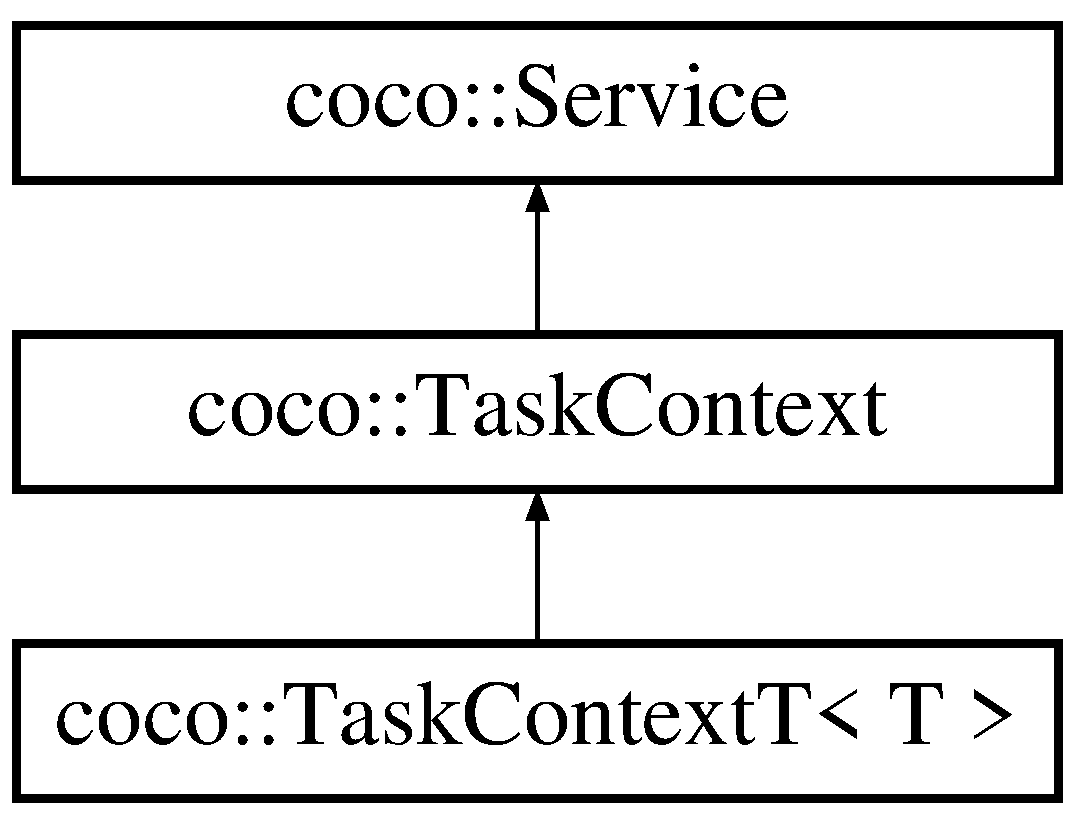
\includegraphics[height=4.000000cm]{classcoco_1_1_task_context}
\end{center}
\end{figure}
\subsection*{Public Member Functions}
\begin{DoxyCompactItemize}
\item 
\hypertarget{classcoco_1_1_task_context_a66769b9863ddc426776f67905b9cbfc2}{}void \hyperlink{classcoco_1_1_task_context_a66769b9863ddc426776f67905b9cbfc2}{set\+Activity} (\hyperlink{classcoco_1_1_activity}{Activity} $\ast$activity)\label{classcoco_1_1_task_context_a66769b9863ddc426776f67905b9cbfc2}

\begin{DoxyCompactList}\small\item\em Set the activity that will manage the execution of this task. \end{DoxyCompactList}\item 
\hypertarget{classcoco_1_1_task_context_a1e631768ca31e55c4c2605320df997fc}{}virtual void \hyperlink{classcoco_1_1_task_context_a1e631768ca31e55c4c2605320df997fc}{start} ()\label{classcoco_1_1_task_context_a1e631768ca31e55c4c2605320df997fc}

\begin{DoxyCompactList}\small\item\em Start the execution. \end{DoxyCompactList}\item 
\hypertarget{classcoco_1_1_task_context_ae8fe9cb7eec3d3f57d57cd692e781785}{}virtual void \hyperlink{classcoco_1_1_task_context_ae8fe9cb7eec3d3f57d57cd692e781785}{stop} ()\label{classcoco_1_1_task_context_ae8fe9cb7eec3d3f57d57cd692e781785}

\begin{DoxyCompactList}\small\item\em Stop the execution of the component. \end{DoxyCompactList}\item 
\hypertarget{classcoco_1_1_task_context_a72a5550fc3d0ceba03f8b091852d71f6}{}virtual void \hyperlink{classcoco_1_1_task_context_a72a5550fc3d0ceba03f8b091852d71f6}{trigger\+Activity} ()\label{classcoco_1_1_task_context_a72a5550fc3d0ceba03f8b091852d71f6}

\begin{DoxyCompactList}\small\item\em In case of a T\+R\+I\+G\+G\+E\+R task execute one step. \end{DoxyCompactList}\item 
\hypertarget{classcoco_1_1_task_context_a66ec10f5b0f28a717cdc9c76110441fd}{}virtual const std\+::type\+\_\+info \& {\bfseries type} () const =0\label{classcoco_1_1_task_context_a66ec10f5b0f28a717cdc9c76110441fd}

\item 
\hypertarget{classcoco_1_1_task_context_a7d7947be2c6466cbae938958bf147c5a}{}std\+::shared\+\_\+ptr$<$ \hyperlink{classcoco_1_1_execution_engine}{Execution\+Engine} $>$ {\bfseries engine} () const \label{classcoco_1_1_task_context_a7d7947be2c6466cbae938958bf147c5a}

\end{DoxyCompactItemize}
\subsection*{Protected Member Functions}
\begin{DoxyCompactItemize}
\item 
\hypertarget{classcoco_1_1_task_context_a2254f581ed334e5273246e88c05ddfed}{}\hyperlink{classcoco_1_1_task_context_a2254f581ed334e5273246e88c05ddfed}{Task\+Context} ()\label{classcoco_1_1_task_context_a2254f581ed334e5273246e88c05ddfed}

\begin{DoxyCompactList}\small\item\em Creates an \hyperlink{classcoco_1_1_execution_engine}{Execution\+Engine} object. \end{DoxyCompactList}\item 
\hypertarget{classcoco_1_1_task_context_adb443956ebfd96472f7a8ed0e4042054}{}virtual std\+::string {\bfseries info} ()=0\label{classcoco_1_1_task_context_adb443956ebfd96472f7a8ed0e4042054}

\item 
\hypertarget{classcoco_1_1_task_context_a4ac24bd71202d3e87d487dd24d47d9a0}{}virtual void \hyperlink{classcoco_1_1_task_context_a4ac24bd71202d3e87d487dd24d47d9a0}{init} ()=0\label{classcoco_1_1_task_context_a4ac24bd71202d3e87d487dd24d47d9a0}

\begin{DoxyCompactList}\small\item\em Init the task attributes and properties, called by the instantiator before spawing the thread. \end{DoxyCompactList}\item 
\hypertarget{classcoco_1_1_task_context_a397ba5231353db343c71280ca0502459}{}virtual void \hyperlink{classcoco_1_1_task_context_a397ba5231353db343c71280ca0502459}{on\+Config} ()=0\label{classcoco_1_1_task_context_a397ba5231353db343c71280ca0502459}

\begin{DoxyCompactList}\small\item\em Function to be overload by the user. It is called once as the thread starts. \end{DoxyCompactList}\item 
\hypertarget{classcoco_1_1_task_context_a75a4efc25d04977d15bfdd8407d29d07}{}virtual void \hyperlink{classcoco_1_1_task_context_a75a4efc25d04977d15bfdd8407d29d07}{on\+Update} ()=0\label{classcoco_1_1_task_context_a75a4efc25d04977d15bfdd8407d29d07}

\begin{DoxyCompactList}\small\item\em Function to be overload by the user. It is the execution funciton. \end{DoxyCompactList}\end{DoxyCompactItemize}
\subsection*{Protected Attributes}
\begin{DoxyCompactItemize}
\item 
\hypertarget{classcoco_1_1_task_context_a7f6706f1339e8c6e8972c3c9244d5efe}{}std\+::shared\+\_\+ptr$<$ \hyperlink{classcoco_1_1_execution_engine}{Execution\+Engine} $>$ {\bfseries engine\+\_\+}\label{classcoco_1_1_task_context_a7f6706f1339e8c6e8972c3c9244d5efe}

\end{DoxyCompactItemize}
\subsection*{Private Attributes}
\begin{DoxyCompactItemize}
\item 
\hypertarget{classcoco_1_1_task_context_a3e64c0ed592191c264ccb5705e17dfcc}{}\hyperlink{classcoco_1_1_activity}{Activity} $\ast$ {\bfseries activity\+\_\+}\label{classcoco_1_1_task_context_a3e64c0ed592191c264ccb5705e17dfcc}

\item 
\hypertarget{classcoco_1_1_task_context_a47d34de836289ab6a137c8e0d584bcc0}{}\hyperlink{namespacecoco_afec53814046619bac93c2077706a6bd1}{Task\+State} {\bfseries state\+\_\+}\label{classcoco_1_1_task_context_a47d34de836289ab6a137c8e0d584bcc0}

\end{DoxyCompactItemize}
\subsection*{Friends}
\begin{DoxyCompactItemize}
\item 
\hypertarget{classcoco_1_1_task_context_ab80f178dab101a5299f5ebd3d78bef93}{}class {\bfseries Coco\+Launcher}\label{classcoco_1_1_task_context_ab80f178dab101a5299f5ebd3d78bef93}

\item 
\hypertarget{classcoco_1_1_task_context_af18a9ee98e70982bfe2975391d7221a5}{}class {\bfseries System}\label{classcoco_1_1_task_context_af18a9ee98e70982bfe2975391d7221a5}

\item 
\hypertarget{classcoco_1_1_task_context_a9b68196ad6ed6fa11eb4454434b39bb5}{}class {\bfseries Execution\+Engine}\label{classcoco_1_1_task_context_a9b68196ad6ed6fa11eb4454434b39bb5}

\end{DoxyCompactItemize}


\subsection{Detailed Description}
The Task Context is the single task of the Component being instantiated

A Task Context provides\+:
\begin{DoxyItemize}
\item operators
\item input ports
\item output ports
\item parameters (config time)
\item properties (run time) 
\end{DoxyItemize}

The documentation for this class was generated from the following files\+:\begin{DoxyCompactItemize}
\item 
src/coco\+\_\+core.\+hpp\item 
src/coco\+\_\+core.\+cpp\end{DoxyCompactItemize}

\hypertarget{classcoco_1_1_task_context_t}{\section{coco\-:\-:Task\-Context\-T$<$ T $>$ Class Template Reference}
\label{classcoco_1_1_task_context_t}\index{coco\-::\-Task\-Context\-T$<$ T $>$@{coco\-::\-Task\-Context\-T$<$ T $>$}}
}
Inheritance diagram for coco\-:\-:Task\-Context\-T$<$ T $>$\-:\begin{figure}[H]
\begin{center}
\leavevmode
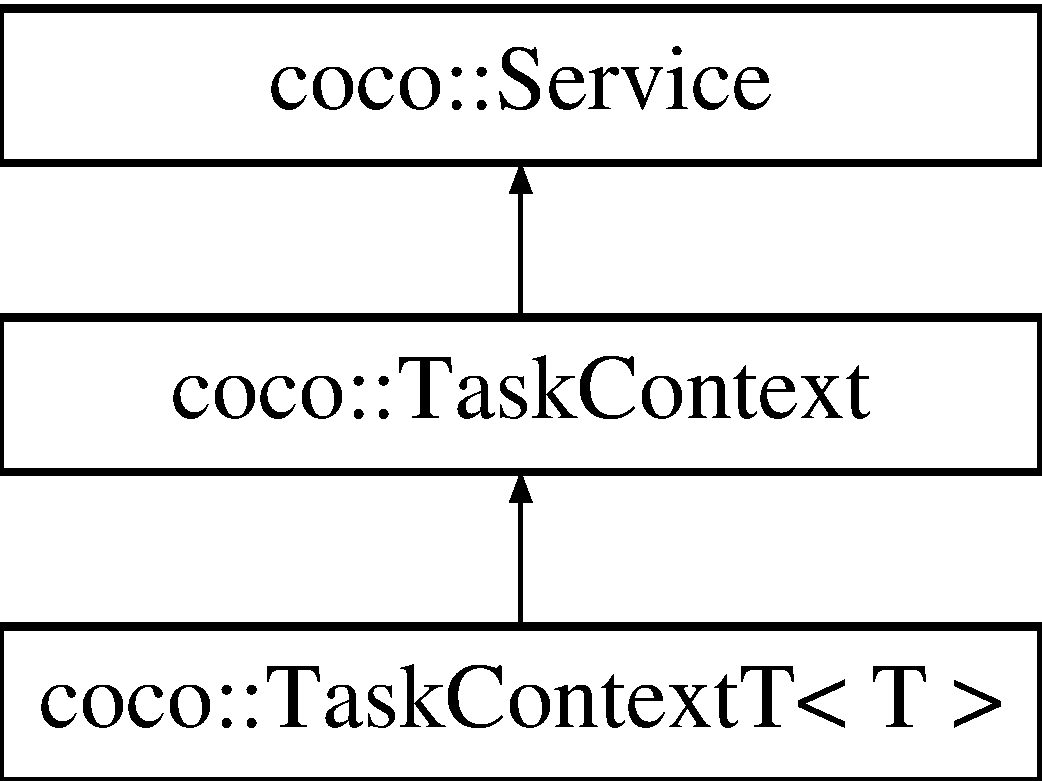
\includegraphics[height=3.000000cm]{classcoco_1_1_task_context_t}
\end{center}
\end{figure}
\subsection*{Public Member Functions}
\begin{DoxyCompactItemize}
\item 
\hypertarget{classcoco_1_1_task_context_t_a0cd1cf23e0679a4dc147ac8716dafea0}{virtual const std\-::type\-\_\-info \& {\bfseries type} () const override}\label{classcoco_1_1_task_context_t_a0cd1cf23e0679a4dc147ac8716dafea0}

\end{DoxyCompactItemize}
\subsection*{Additional Inherited Members}


The documentation for this class was generated from the following file\-:\begin{DoxyCompactItemize}
\item 
src/ezoro.\-hpp\end{DoxyCompactItemize}

\input{classcoco_1_1_timer}
\input{classcoco_1_1_timer_manager}
%--- End generated contents ---

% Index
\backmatter
\newpage
\phantomsection
\clearemptydoublepage
\addcontentsline{toc}{chapter}{Index}
\printindex

\end{document}
